\documentclass{article}
\usepackage[letterpaper, top=1in, bottom=1in, left=1in, right=1in]{geometry}
\usepackage[utf8]{inputenc}



\usepackage[english]{babel}
\usepackage{tikz-cd,lipsum, bm, dcolumn, lastpage, pgfplots}
\pgfplotsset{compat=1.18}
\usetikzlibrary{arrows}
\usepackage{amsmath, amssymb, amsthm, mathrsfs, mathtools, centernot, hyperref, fancyhdr, lastpage}
\usepackage{graphicx} 
\usepackage{caption, subcaption}
\usepackage{enumitem, tikz}
\usepackage{fancyvrb,newverbs,xcolor}
\usetikzlibrary{positioning}
\definecolor{cverbbg}{gray}{0.93}

\newenvironment{cverbatim}
 {\SaveVerbatim{cverb}}
 {\endSaveVerbatim
  \flushleft\fboxrule=0pt\fboxsep=.5em
  \colorbox{cverbbg}{%
    \makebox[\dimexpr\linewidth-2\fboxsep][l]{\BUseVerbatim{cverb}}%
  }
  \endflushleft
}

\renewcommand{\thispagestyle}[1]{}

\DeclareMathOperator{\Tr}{Tr}
\DeclareMathOperator{\Sym}{Sym}
\DeclareMathOperator{\Span}{span}
\DeclareMathOperator{\std}{std}
\DeclareMathOperator{\Cov}{Cov}
\DeclareMathOperator{\Var}{Var}
\DeclareMathOperator{\Corr}{Corr}
\DeclareMathOperator*{\argmin}{\arg\!\min}
\DeclareMathOperator*{\argmax}{\arg\!\max}

\theoremstyle{definition}
\newtheorem{theorem}{Theorem}[section]
\newtheorem{proposition}[theorem]{Proposition}
\newtheorem{lemma}[theorem]{Lemma}
\newtheorem{example}{Example}[section]
\newtheorem{exercise}{Exercise}[section]
\newtheorem{corollary}{Corollary}[theorem]
\theoremstyle{remark}
\newtheorem*{remark}{Remark}
\theoremstyle{definition}
\newtheorem{definition}{Definition}[section]
\renewcommand{\qed}{\hfill$\blacksquare$}
\renewcommand{\footrulewidth}{0.4pt}% default is 0pt

\newenvironment{solution}{\noindent \textit{Solution.}}{}

\renewcommand{\thispagestyle}[1]{}

\begin{document}
\pagestyle{fancy}

\lhead{Deep Learning}
\chead{Muchang Bahng}
\rhead{\date{Summer 2023}}
\cfoot{\thepage / \pageref{LastPage}}

\title{Deep Learning}
\author{Muchang Bahng}
\date{Summer 2023}

\maketitle

\tableofcontents

\pagebreak 

This requires you to know both the supervised and unsupervised learning notes, especially on generalized linear models. We will use PyTorch. 

\section{Multi-Layered Perceptrons}

\subsection{Generalized Linear Models}

First, we transform the inputs into the relevant features $\mathbf{x}_n \mapsto \boldsymbol{\phi} (\mathbf{x}_n) = \boldsymbol{\phi}_n$ and then, when we construct a generalized linear model, we assume that the conditional distribution $Y \mid X = x$ is in the canonical exponential family, with some natural parameter $\eta(x)$ and expected mean $\mu(x) = \mathbb{E}[Y \mid X = x]$. Then, to choose the link function $g$ that related $g(\mu(x)) = x^T \beta$, we can set it to be the canonical link $g$ that maps $\mu$ to $\eta$. That is, 
\[g(\mu(x)) = x^T \beta = \eta (x)\]
such that the natural parameter is linearly dependent on the input. The inverse $g^{-1}$ of the link function is called the \textbf{activation function}, which connects the expected mean to a linear function of $x$. 
\[h_\beta (x) = g^{-1} (x^T \beta) = \mu(x) = \mathbb{E}[Y \mid X = x]\]
Now, note that for a classification problem, the decision boundary defined in the $\boldsymbol{\phi}$ feature space is linear, but it may not be linear in the input space $\mathcal{X}$. For example, consider the set of points in $\mathbb{R}^2$ with the corresponding class in $\ref{fig:logistic_transformed}$. We transform the features to $\boldsymbol{\phi}(x_1, x_2) = x_1^2 + x_2^2$, which gives us a new space to work with. Fitting logistic regression onto this gives a linear decision boundary in the space $\boldsymbol{\phi}$, but the boundary is circular in $\mathcal{X} = \mathbb{R}^2$. 

\begin{figure}[hbt!]
    \centering
    \begin{subfigure}[b]{0.35\textwidth}
    \centering
        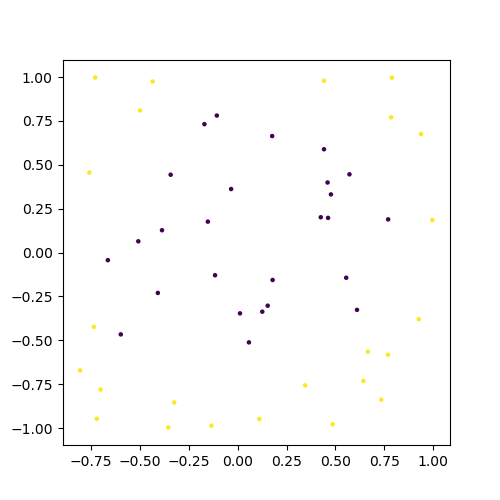
\includegraphics[width=\textwidth]{Images/logistic/untrans_data.png}
        \caption{Data in space $\mathcal{X} = \mathbb{R}^2$. }
        \label{fig:raw_points}
    \end{subfigure}
    \begin{subfigure}[b]{0.35\textwidth}
    \centering
        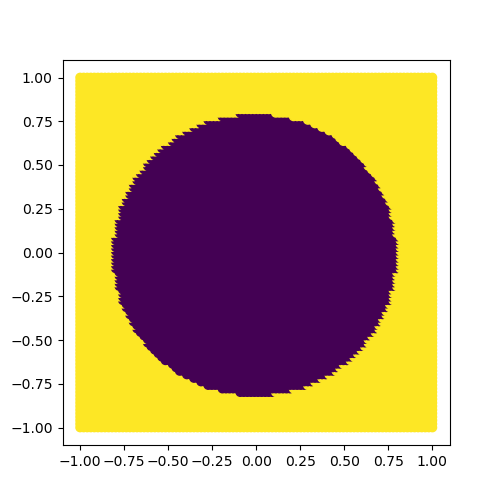
\includegraphics[width=\textwidth]{Images/logistic/untrans_fit.png}
        \caption{Logistic fit to data in input space. }
        \label{fig:raw_trained}
    \end{subfigure}

    \centering
    \begin{subfigure}[b]{0.35\textwidth}
    \centering
        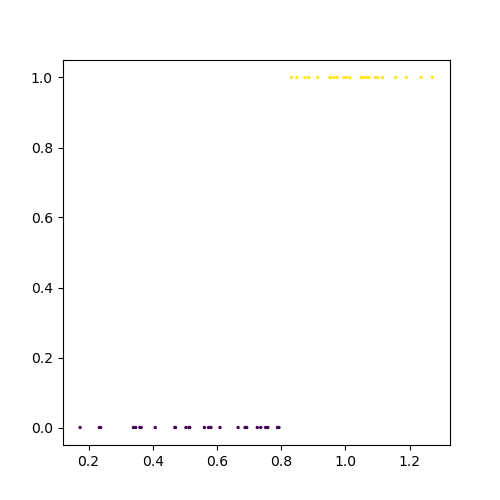
\includegraphics[width=\textwidth]{Images/logistic/trans_data.png}
        \caption{Transformed data $\phi(\mathbf{x}) = ||\mathbf{x}||$. }
        \label{fig:transformed_points}
    \end{subfigure}
    \begin{subfigure}[b]{0.35\textwidth}
    \centering
        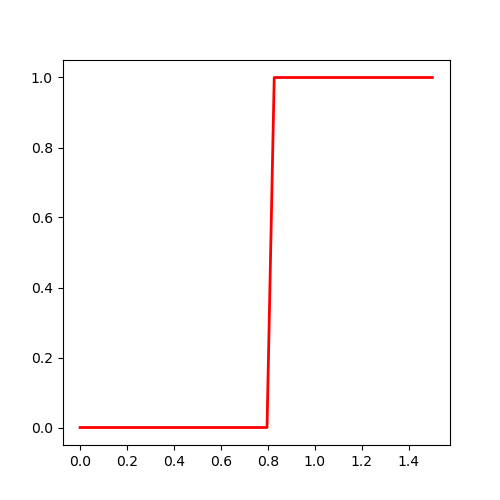
\includegraphics[width=\textwidth]{Images/logistic/trans_fit.png}
        \caption{Logistic fit in transformed space. }
        \label{fig:transformed_trained}
    \end{subfigure}
    \caption{A nonlinear feature transformation $\phi$ will cause a nonlinear decision boundary when doing logistic regression. }
    \label{fig:logistic_transformed}
\end{figure}

\begin{example}[Tarokh, ECE685 2021 Midterm 1]
Let $x \in \mathbb{R}$ denote a random variable with the following \textit{cumulative distribution function} 
\[F(x) = \exp \bigg( - \exp \bigg( - \frac{x - \mu}{\beta} \bigg) \bigg) \] 
where $\mu$ and $\beta > 0$ denote the location and scale parameters, respectively. Let $\mathcal{D} = \{x_1, \ldots, x_n\}$ be a set of $n$ iid observations of $x$. 
\begin{enumerate}
    \item Write an equation for a cost function $L(\mu, \beta \mid \mathcal{D})$ whose minimization gives the maximum likelihood estimates for $\mu$ and $\beta$. 
    \item Compute the derivatives of $L(\mu, \beta \mid \mathcal{D})$ with respect to $\mu$ and $\beta$ and write a system of equations whose solution gives the MLEs of $\mu$ and $\beta$. 
\end{enumerate}
\end{example}

\begin{solution}
We can derive the PDF of the observation as 
\[f(x; \mu, \beta) = \frac{d F(x)}{dx} = \frac{1}{\beta} \exp \bigg\{ - \bigg( \frac{x - \mu}{\beta} + \exp \Big( - \frac{x - \mu}{\beta}\Big) \bigg) \bigg\}\] 
and the likelihood is then 
\begin{align*}
    L(\mu, \beta \mid \mathcal{D}) & = \prod_{i=1}^N \frac{1}{\beta} \exp \bigg\{ - \bigg( \frac{x^{(i)} - \mu}{\beta} + \exp \Big( - \frac{x^{(i)} - \mu}{\beta}\Big) \bigg) \bigg\}
\end{align*}
Rather than maximizing this likelihood, we minimize the negative log of it, defined as 
\[ \ell(\mu, \beta \mid \mathcal{D}) = - \ln L(\mu, \beta \mid \mathcal{D}) = N \ln{\beta} + \frac{\sum_{i} x^{(I)} - N \mu}{\beta} + \sum_{i=1}^N \exp \Big( - \frac{x^{(i)} - \mu}{\beta} \Big) \]    
The derivatives of $\ell$ can be computed simply by using the derivative rules.  
\begin{align*}
    \frac{\partial \ell}{\partial \mu} & = - \frac{N}{\beta} + \frac{1}{\beta} \sum_{i=1}^N \exp \Big( - \frac{x^{(i)} - \mu}{\beta} \Big) \\
    \frac{\partial \ell}{\partial \beta} & = \frac{N}{\beta} - \frac{\sum_{i} x^{(i)} - N \mu}{\beta^2} + \frac{1}{\beta^2} \sum_{i=1}^N (x^{(i)} - \mu) \exp \Big( - \frac{x^{(i)} - \mu}{\beta} \Big)
\end{align*}
and so the MLE estimates that minimizes $\ell$ can be found by setting the equations above equal to $0$. 
\end{solution}

We would like to extend this model by making the basis functions $\boldsymbol{\phi}_n$ depend on the parameters $\mathbf{w}$ and then allow these parameters to be adjusted during training. There are many ways to construct parametric nonlinear basis functions and in fact, neural networks use basis functions that are of the form $\boldsymbol{\phi}(\mathbf{x}) = g^{-1} (\mathbf{x}^T \boldsymbol{\beta})$. 

\subsection{Architecture}

A neuron basically takes in a vector $\mathbf{x} \in \mathbb{R}^d$ and multiplies its corresponding weight by some vector $\boldsymbol{\omega}$, plus some bias term $b$. It is then sent into some nonlinear activation function $\sigma: \mathbb{R} \longrightarrow \mathbb{R}$. Letting the parameter be $\theta = (\boldsymbol{\omega}, b)$, we can think of a neuron as a function 
\[h_\theta (\mathbf{x}) = f(\boldsymbol{\omega}^T \mathbf{x} + b) \]
A single neuron with the activation function as the step function 
\[f(z) = \begin{cases} 1 & \text{ if } z \geq 0 \\ 0 & \text{ if } z < 0 \end{cases} \]
is simply the perceptron algorithm. It divides $\mathbb{R}^d$ using a hyperplane $\boldsymbol{\omega}^T \mathbf{x} + b = 0$ and linearly classifies all points on one side to value $1$ and the other side to value $0$. This is similar to a neuron, which takes in a value and outputs a ``signal" if the function evaluated gets past a threshold. However, we would like to use smooth activation functions for this, so we would use different activations. Hence we have a neuron. 

\begin{definition}[Neuron]
A \textbf{neuron} is a function (visualized as a node) that takes in inputs $\mathbf{x}$ and outputs a value $y$ calculated 
\[y = \sigma(\mathbf{w}^T x  + b)\]
where $\sigma$ is an activation function. Activation functions are usually simple functions with a range of $[0, 1]$ or $[-1, 1]$, and popular ones include: 
\begin{enumerate}
    \item the rectified linear unit 
    \[\mathrm{ReLU}(z) = \max\{0 , z\}\]
    \item the sigmoid 
    \[\sigma(z) = \frac{1}{1 + e^{-z}}\]
    \item the hyperbolic tangent 
    \[\tanh(z) = \frac{e^{z} - e^{-z}}{e^z + e^{-z}}\]
\end{enumerate}
A visual of a neuron is shown in Figure \ref{fig:neuron}. 
\begin{figure}
    \centering
    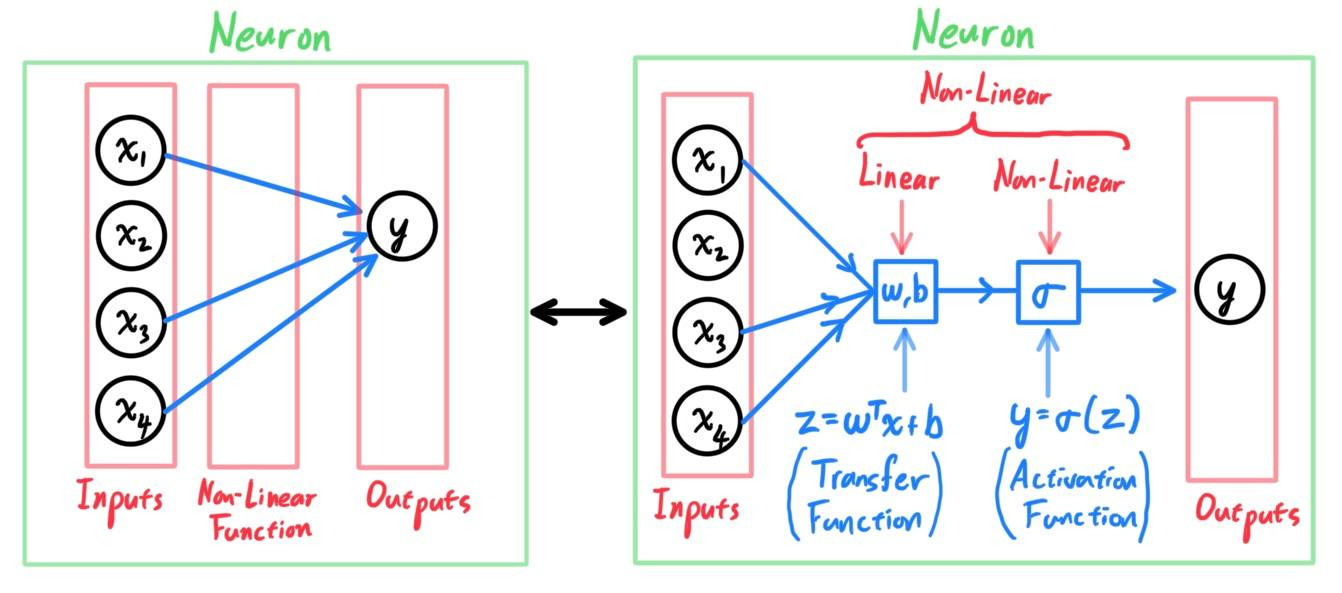
\includegraphics[scale=0.25]{Images/MLP/Neuron.jpg}
    \caption{Diagram of a neuron, decomposed into its linear and nonlinear components. }
    \label{fig:neuron}
\end{figure}
\end{definition}

If there does not exist any arrow from a potential input $\mathbf{x}$ to an output $y$, then this means that $\mathbf{x}$ is not relevant in calculating $y$. However, we usually work with \textbf{fully-connected neural networks}, which means that every input is relevant to calculating every output, since we usually cannot make assumptions about which variables are relevant or not. We can stack multiple neurons such that one neuron passes its output as input into the next neuron, resulting in a more complex function. What we have seen just now is a 1-layer neural network. 

\begin{definition}[Multilayer Perceptron]
A $L$-layer MLP $\mathbf{h}_\theta : \mathbb{R}^D \longrightarrow \mathbb{R}^M$ is the function 
\[h_\theta (\mathbf{x}) \coloneqq \boldsymbol{\sigma}^{[L]} \circ \mathbf{W}^{[L]} \circ \boldsymbol{\sigma}^{[L-1]} \circ \mathbf{W}^{[L-1]} \circ \cdots \circ \boldsymbol{\sigma}^{[1]} \circ \mathbf{W}^{[1]} (\mathbf{x})\]
where $\boldsymbol{\sigma}^{[l]}: \mathbb{R}^{N^{[l]}} \rightarrow \mathbb{R}^{N^{[l]}}$ is an activation function and $\mathbf{W}^{[l]}: \mathbb{R}^{N^{[l-1]}} \rightarrow \mathbb{R}^{N^{[l]}}$ is an affine map. We will use the following notation. 
\begin{enumerate}
    \item The inputs will be labeled $\mathbf{x} = \mathbf{a}^{[0]}$ which is in $\mathbb{R}^{N^{[0]}} = \mathbb{R}^D$. 
    
    \item We map $\mathbf{a}^{[l]} \in \mathbb{R}^{N^{[l]}} \mapsto \mathbf{W}^{[l+1]} \mathbf{a}^{[l]} + \mathbf{b}^{[l+1]}= \mathbf{z}^{[l+1]} \in \mathbb{R}^{N^{[l+1]}}$, where $z$ denotes a vector after an affine transformation. 

    \item We map $\mathbf{z}^{[l+1]} \in \mathbb{R}^{N^{[l+1]}} \mapsto \boldsymbol{\sigma}(\mathbf{z}^{[l+1]}) = \mathbf{a}^{[l+1]} \in \mathbb{R}^{N^{[l+1]}}$, where $a$ denotes a vector after an activation function. 

    \item We keep doing this until we reach the second last layer with vector $\mathbf{a}^{[L-1]}$. 

    \item Now we want our last layer to be our predicted output. Based on our assumptions of the problem, we construct a generalized linear model with some inverse link function $g$. We perform one more affine transformation $\mathbf{a}^{[L-1]} \mapsto \mathbf{W}^{[L]} \mathbf{a}^{[L-1]} + \mathbf{b}^{[L]} = \mathbf{z}^{[L]}$, followed by the link function to get our prediction: $\mathbf{a}^{[L]} = \mathbf{g}(\mathbf{z}^{[L]}) = \mathbf{h}_{\boldsymbol{\theta}} (\mathbf{x}) \in \mathbb{R}^M$. 
\end{enumerate}
All the parameters of the neural net will be denoted $\boldsymbol{\theta}$. 
\begin{center}
    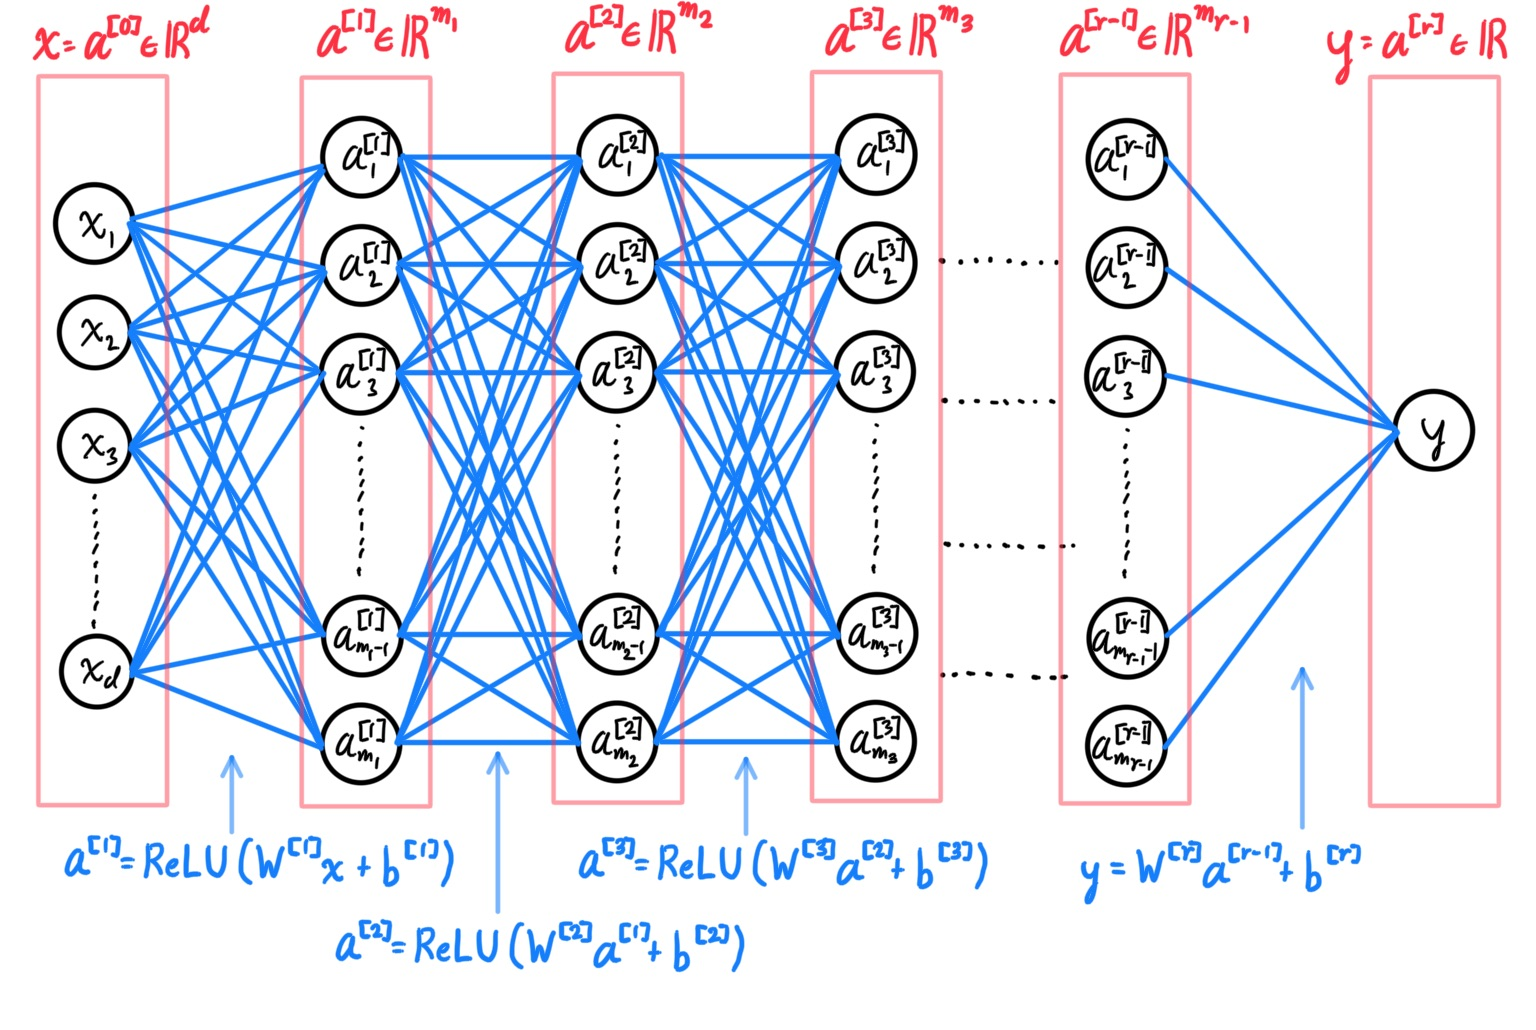
\includegraphics[scale=0.2]{Images/MLP/Multilayer_Neural_Net.jpg}
\end{center}
Ultimately, a neural net is really just a generalized linear model with some trained feature extractors, which is why in practice, if researchers want to predict a smaller dataset, they take a pretrained model on a related larger dataset and simply tune the final layer, since the second last layer most likely encodes all the relevant features. This is called \textbf{transfer learning}. 
\end{definition}



\begin{example}
The \textbf{fully-connected 2-layer neural network} of $d$ input features $\mathbf{x} \in \mathbb{R}^d$ and one scalar output $y \in \mathbb{R}$ can be visualized below. It has one \textbf{hidden layer} with $m$ inputs values $a_1, \ldots, a_m$. 
\begin{center}
    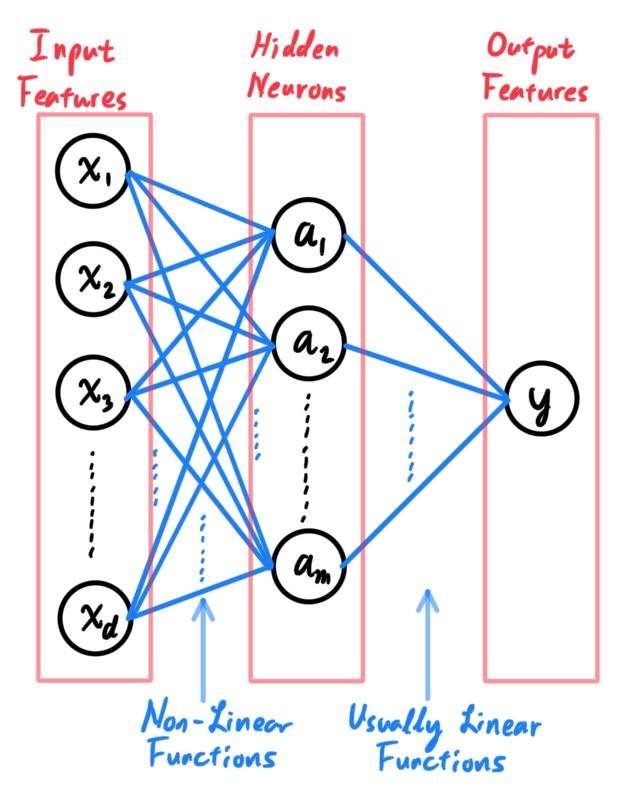
\includegraphics[scale=0.2]{Images/MLP/2_layer_neural_net.jpg}
\end{center}
Conventionally, we account for every layer except for the final layer when talking about the number of layers in the neural net. 
\end{example}

Note that each layer corresponds to how close a neuron is to the output. But really any neuron can be a function of any other neuron. For example, we can connect a neuron from layer $4$ back to a neuron of layer $1$. For now, we will consider networks that are restricted to a \textbf{feed-forward} architecture, in other words having no closed directed cycles. 

\subsection{Universal Approximation Theorem} 

Neural networks have been mathematically studied back in the 1980s, and the reason that they are so powerful is that we can theoretically prove the limits on what they can learn. For very specific classes of functions, the results are easier, but for more general ones, it becomes much harder. We prove one of the theorems below. 

Let us think about how one would construct approximations for such functions. Like in measure theory, we can think of every measurable function as a linear combination of a set of bump functions, and so we can get a neural network to do the same.

\begin{example}[Bump Functions in $\mathbb{R}$] 
Assuming the sigmoid activation function is used, the bump function 
\[f(x) = \begin{cases} 1 & \text{ if } a < x < b \\ 0 & \text{ if else} \end{cases}\]i
can be approximated by taking a linear combination of a sigmoid function stepping up and one stepping down. That is, 
\[f(x) \approx \frac{1}{2} \sigma \big( k( x - a)\big) - \frac{1}{2} \sigma \big( k (x - b) \big)\]
where $k$ is a scaling constant that determines how steep the steps are for each function. Therefore, as $k \rightarrow \infty$, the function begins to look more like a step function. 
\end{example}

\begin{example}[Bump Functions in $\mathbb{R}^2$]
To do this for a 2-D step function, of the form 
\[f(x_1, x_2) = \begin{cases} 1 \text{ if } a < x_1 < b \\ 0 & \text{ if else} \end{cases}\]
this is a simple extension of the first one. We just don't need to make our linear combination dependent on $x_2$ and we're done.
\[f(x) \approx \frac{1}{2} \sigma \big( k( x_1 - a)\big) - \frac{1}{2} \sigma \big( k (x_1 - b) \big)\]

\end{example} 

\begin{example}[Tower Functions in $\mathbb{R}^2$] 
Now to construct a tower function of the form 
\[f(x_1, x_2) = \begin{cases} 1 & \text{ if } a_1 < x_1 < b_1, a_2 < x_2 < b_2 \\ 0 & \text{ if else} \end{cases}\]i
we need slightly more creativity. Now we can approximate it by doing 
\[f(x) \approx \sigma \bigg( k_2 \big[ \sigma\big( k_1 (x_1 - a_1)\big) - \sigma\big( k_1 (x_1 -b_1)\big) + \sigma \big( k_1 (x_2 - a_2)\big) - \sigma\big(k_1 (x_2 - b_2)\big)  big] - b_2\bigg)\]
\end{example} 

At this point, we can see how this would extend to $\mathbb{R}^n$, and by isolating parts of the network we can have it approximate tower functions that are completely separate from each other, at any height, and then finally take a linear combination of them to approximate the original function of interest.  

\begin{theorem}[CS671 Fall 2023 Problem Set 5]
Suppose you have a 2D, $L$-lipschitz function $f(x_1, x_2)$ defined on a unit square ($x_1, x_2 \in \left [0,1 \right ]$). You want to approximate this with an arbitrary neural net $\Tilde{f}$ such that
\[\sup_{x \in [0, 1]^2} |f(x) - \Tilde{f}(x)| \leq \epsilon\]    
If we divide the square into a checkerboard of $K \times K$ nonoverlapping squares, approximate the restriction of $f$ to each subsquare with a tower function, what is the least $K$ we would need to ensure that the error is less than $\epsilon$? 
\end{theorem} 


\subsection{Forward and Back Propagation}

Back in the supervised learning notes, we have gone through the derivation for linear, logistic, and softmax regression. It turns out that despite them having very different architectures, with a identity, sigmoid, and softmax activation function, our choice of loss to be the mean squared loss, the binary cross-entropy, and the cross-entropy loss, had given very cute formulas in computing the gradient of the loss. Unfortunately, the formulas do not get cute when we differentiate neural networks, but they do come in a very structured way. Let us go through a very simple example to gain intuition. 

\begin{example}[ECE 685 Fall 2021 Midterm 1]
The figure depicts a simple neural network with one hidden layer. The inputs to the network are denoted by $x_1, x_2, x_3$, and the output is denoted by $y$. The activation functions of the neurons in the hidden layer are given by $h_1 (z) = \sigma(z), h_2 (z) = \tanh(z)$, and the output unit activation function is $g(z) = z$, where $\sigma(z) = \frac{1}{1 + \exp(-z)}$ and $\tanh(z) = \frac{\exp(z) - \exp(-z)}{\exp(z) + \exp(-z)}$ are the logistic sigmoid and hyperbolic tangent, respectively. The biases $b_1, b_2$ are added to the inputs of the neurons int he hidden layer before passing them through the activation functions. let 
\[\mathbf{w} = (b_1, b_2, w_{11}^{(1)}, w_{12}^{(1)}, w_{21}^{(1)}, w_{31}^{(1)}, w_{32}^{(1)}, w_1^{(2)}, w_2^{(2)}) \] 
denote the vector of network parameters. 
\begin{enumerate}
    \item Write the input output relation $y = f(x_1, x_2, x_3 ; \mathbf{w})$ in explicit form. 
    \item Let $\mathcal{D} = \{(x_{1, n}, x_{2, n}, x_{3, n})\}$ denote a training dataset of $N$ points where $y_n \in \mathbb{R}$ are labels of the corresponding data points. We want to estimate the network parameters $\mathbf{w}$ using $\mathcal{D}$ by minimizing the mean squared error loss 
    \[ L(\mathbf{w}) = \frac{1}{2} \sum_{n=1}^N \big( f(x_{1, n}, x_{2, n}, x_{3, n}; \mathbf{w}) - y_n \big)^2 \]
    Compute the gradient of $L(\mathbf{w})$ with respect to the network parameters $\mathbf{w}$. 


    \item Write pseudo code for one iteration for minimizing $L(\mathbf{w})$ with respect to the network parameters $\mathbf{w}$ using SGD with learning rate $\eta > 0$. 
\end{enumerate}

\begin{center}
    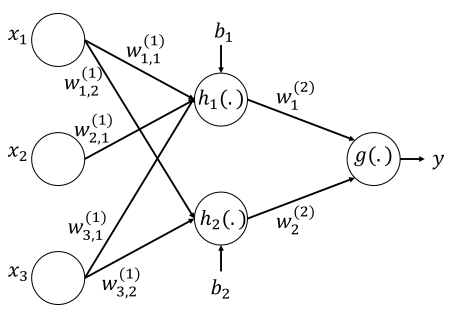
\includegraphics[scale=0.4]{Images/tarokhfig1.png}
\end{center}
\end{example}
\begin{solution}
We can write the computation graph as 
\begin{align*} 
    z_1^{(1)} & = w_{11}^{(1)} x_1 + w_{21}^{(1)} x_2 + w_{31}^{(1)} x_3 + b_1 \\
    z_2^{(1)} & = w_{12}^{(1)} x_1 + w_{32}^{(1)} x_3 + b_2 \\
    a_1^{(1)} & = \sigma(z^{(1)})\\
    a_2^{(1)} & = \tanh(z_2^{(1)}) \\
    z^{(2)} & = w_{1}^{(2)} a_1^{(1)} + w_2^{(2)} a_2^{(1)} \\
    y = a^{(2)} & = g(z^{(2)})
\end{align*}
and composing these gives 
\[y = w_1^{(2)} \sigma(w_{11}^{(1)} x_1  + w_{21}^{(1)} x_2 + w_{31}^{(1)} x_3 + b_1) + w_2^{(2)} \tanh(w_{12}^{(1)} x_1 + w_{32}^{(1)} x_3 + b_2) \]
The gradient of the network can be written as 
\begin{align*}
    \nabla_\mathbf{w} L(\mathbf{w}) & = \frac{1}{2} \sum_{n=1}^N \nabla_\mathbf{w} \big( f(x_{1, n}, x_{2, n}, x_{3, n}; \mathbf{w}) - y_n \big)^2 \\
    & = \sum_{n=1}^N (f(x_{1, n}, x_{2, n}, x_{3, n}; \mathbf{w}) - y_n) \nabla_\mathbf{w} f(x_{1, n}, x_{2, n}, x_{3, n})
\end{align*}
where 
\[\nabla_\mathbf{w} f(x_{1, n}, x_{2, n}, x_{3, n}) = \frac{\partial f}{\partial \mathbf{w}} \bigg|_{\mathbf{x} = \mathbf{x}^{(n)}}\] 
Now we can take derivatives using chain rule, working backwards, and using the derivative identities $\sigma^\prime (z)  = \sigma(z) (1 - \sigma(z))$ and $\tanh^\prime (z) = 1 - \tanh^2 (z)$. 
\begin{align*}
    \frac{\partial f}{\partial w_1^{(2)}} & = \frac{\partial f}{\partial z^{(2)}} \frac{\partial z^{(2)}}{\partial w_1^{(2)}} = a_1^{(1)} \\
    \frac{\partial f}{\partial w_2^{(2)}} & = \frac{\partial f}{\partial z^{(2)}} \frac{\partial z^{(2)}}{\partial w_2^{(2)}} = a_2^{(1)} \\ 
    \frac{\partial f}{\partial w_{11}^{(1)}} & = \frac{\partial f}{\partial z^{(2)}} \frac{\partial z^{(2)}}{\partial a^{(1)}_1} \frac{\partial a^{(1)}_1}{\partial z_1^{(1)}} \frac{\partial z_1^{(1)}}{\partial w_{11}^{(1)}} = w_1^{(2)} a_1^{(1)} (1 - a_1^{(1)}) x_1\\
    \frac{\partial f}{\partial w_{21}^{(1)}} & = \frac{\partial f}{\partial z^{(2)}} \frac{\partial z^{(2)}}{\partial a^{(1)}_1} \frac{\partial a^{(1)}_1}{\partial z_1^{(1)}} \frac{\partial z_1^{(1)}}{\partial w_{21}^{(1)}} = w_1^{(2)} a_1^{(1)} (1 - a_1^{(1)}) x_2\\
    \frac{\partial f}{\partial w_{31}^{(1)}} & = \frac{\partial f}{\partial z^{(2)}} \frac{\partial z^{(2)}}{\partial a^{(1)}_1} \frac{\partial a^{(1)}_1}{\partial z_1^{(1)}} \frac{\partial z_1^{(1)}}{\partial w_{31}^{(1)}} = w_1^{(2)} a_1^{(1)} (1 - a_1^{(1)}) x_3\\
    \frac{\partial f}{\partial b_{1}} & = \frac{\partial f}{\partial z^{(2)}} \frac{\partial z^{(2)}}{\partial a^{(1)}_1} \frac{\partial a^{(1)}_1}{\partial z_1^{(1)}} \frac{\partial z_1^{(1)}}{\partial b_{1}}  = w_1^{(2)} a_1^{(1)} (1 - a_1^{(1)}) \\
    \frac{\partial f}{\partial w_{12}^{(1)}} & = \frac{\partial f}{\partial z^{(2)}} \frac{\partial z^{(2)}}{\partial a^{(1)}_2} \frac{\partial a^{(1)}_2}{\partial z_2^{(1)}} \frac{\partial z_2^{(1)}}{\partial w_{12}^{(1)}} = w_2^{(2)} (1 - (a_2^{(1)})^2 ) x_1\\
    \frac{\partial f}{\partial w_{13}^{(1)}} & = \frac{\partial f}{\partial z^{(2)}} \frac{\partial z^{(2)}}{\partial a^{(1)}_2} \frac{\partial a^{(1)}_2}{\partial z_2^{(1)}} \frac{\partial z_2^{(1)}}{\partial w_{13}^{(1)}} = w_2^{(2)} (1 - (a_2^{(1)})^2 ) x_3 \\
    \frac{\partial f}{\partial b_{2}} & = \frac{\partial f}{\partial z^{(2)}} \frac{\partial z^{(2)}}{\partial a^{(1)}_2} \frac{\partial a^{(1)}_2}{\partial z_2^{(1)}} \frac{\partial z_2^{(1)}}{\partial b_{2}} = w_2^{(2)} (1 - (a_2^{(1)})^2 )
\end{align*}
To compute one step of SGD, we must first choose a minibatch $\mathcal{M} \subset \mathcal{D}$ and then compute 
\[\nabla_{\mathbf{w}; \mathcal{M}} L(\mathbf{w}) = \sum_{(\mathbf{x}, y) \in \mathcal{M}} (f(\mathbf{x}; \mathbf{w}) - y) \nabla_{\mathbf{w}} f(\mathbf{x})\] 
where we compute the gradient simply over the minibatch. Then, we update the parameters according to 
\[\mathbf{w} = \mathbf{w} - \eta \nabla_{\mathbf{w}; \mathcal{M}} L(\mathbf{w}) \]
\end{solution}

The following example is slightly harder since we are dealing with fully connected networks. 

\begin{example}
Given the following neural network with 2 inputs $(x_1, x_2)$, fully-connected layers and ReLU activations. The weights and biases of hidden units are denoted $w$ and $b$, with $h$ as activation units. For example, 
\[h_1 = \mathrm{ReLU}(x_1 w_{11} + x_2 w_{21} + b_1) \]
The outputs are denoted as $(y_1, y_2)$ and the ground truth targets are denoted as $(t_1, t_2)$. 
\[y_1  = \mathrm{ReLU} (h_1 w_{31} + h_2 w_{41} + b_3)\]
\begin{center}
    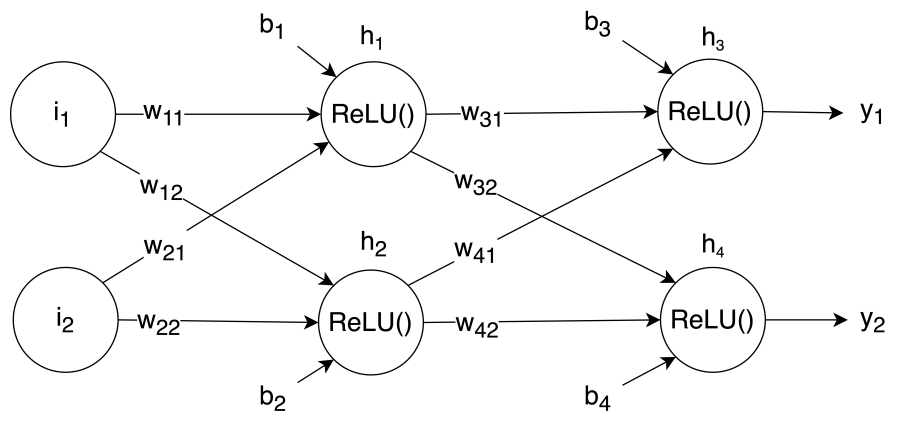
\includegraphics[scale=0.3]{Images/nn_example.png} 
\end{center}
The values of the variables are given as follows: 
\begin{table}[h]
    \centering
    \begin{tabular}{|c|c|c|c|c|c|c|c|c|c|c|c|c|c|c|c|}
        \hline
        $i_1$ & $i_2$ & $w_{11}$ & $w_{12}$ & $w_{21}$ & $w_{22}$ & $w_{31}$ & $w_{32}$ & $w_{41}$ & $w_{42}$ & $b_1$ & $b_2$ & $b_3$ & $b_4$ & $t_1$ & $t_2$ \\
        \hline
        1 & 2 & 1 & 0.5 & -0.5 & 1 & 0.5 & -2 & -1 & 0.5 & -0.5 & -0.5 & 1 & 1 & 2 & 4 \\
        \hline
    \end{tabular}
\end{table}
\begin{enumerate}
    \item Compute the output $(y_1, y_2)$ of the input $(x_1, x_2)$ using the network parameters as specified above. 
    \item Compute the mean squared error of the computed output and the target labels. 
    \item Using the calculated MSE, update the weight $w_{31}$ using GD with $\eta = 0.01$. 
    \item Do the same with weight $w_{42}$. 
    \item Do the same with weight $w_{22}$.  
\end{enumerate}
\end{example}
 

Note that the calculations above require us to compute all the $\mathbf{z}^{(i)}$'s and the $\mathbf{a}^{(i)}$'s, a process called \textbf{forward propagation}, before we compute the gradients. Even in the backpropagation step, we can see that the intermediate partial derivatives in the chain rule are repeatedly used. 


Backpropagation is not hard, but it is cumbersome notation-wise. What we really want to do is just compute a very long vector with all of its partials $\partial E / \partial \boldsymbol{\theta}$. 

To compute $\frac{\partial E_n}{\partial w_{ji}^{[l]}}$, it would be natural to split it up into a portion where $E_n$ is affected by the term before activation $\mathbf{z}^{[l]}$ and how that is affected by $w_{ji}^{[l]}$. The same goes for the bias terms. 
\[\frac{\partial E_n}{\partial w_{ji}^{[l]}} = \underbrace{\frac{\partial E_n}{\partial \mathbf{z}^{[l]}}}_{1 \times N^{[l]}} \cdot \underbrace{\frac{\partial \mathbf{z}^{[l]}}{\partial w_{ji}^{[l]}}}_{N^{[l]} \times 1} \text{ and } \frac{\partial E_n}{\partial b_{i}^{[l]}} = \underbrace{\frac{\partial E_n}{\partial \mathbf{z}^{[l]}}}_{1 \times N^{[l]}} \cdot \underbrace{\frac{\partial \mathbf{z}^{[l]}}{\partial b_{i}^{[l]}}}_{N^{[l]} \times 1}\]
It helps to visualize that we are focusing on 
\[\mathbf{h}_{\boldsymbol{\theta}} (\mathbf{x}) = g\big( \ldots \sigma( \underbrace{\mathbf{W}^{[l]} \mathbf{a}^{[l-1]} + \mathbf{b}^{[l]}}_{\mathbf{z}^{[l]}} )  \ldots \big)\]
We can expand $\mathbf{z}^{[l]}$ to get 
\[\mathbf{z}^{[l]} = \begin{pmatrix} w_{11}^{[l]} & \ldots & w_{1 N^{[l-1]}}^{[l]} \\ \vdots & \ddots & \vdots \\ w_{N^{[l]} 1}^{[l]} & \ldots & w_{N^{[l]} N^{[l-1]}}^{[l]} \end{pmatrix} \begin{pmatrix} a^{[l-1]}_1 \\ \vdots \\ a^{[l-1]}_{N^{[l-1]}} \end{pmatrix} + \begin{pmatrix} b_1^{[l]} \\ \vdots \\ b_{N^{[l]}_{[l]}} \end{pmatrix}\]
$w_{ji}^{[l]}$ will only show up in the $j$th term of $\mathbf{z}^{[l]}$, and so the rest of the terms in $\frac{\partial \mathbf{z}^{[l]}}{\partial w_{ji}^{[l]}}$ will vanish. The same logic applies to $\frac{\partial \mathbf{z}^{[l]}}{\partial b_{i}^{[l]}}$, and so we really just have to compute 
\[\frac{\partial E_n}{\partial w_{ji}^{[l]}} = \underbrace{\frac{\partial E_n}{\partial z^{[l]}_j}}_{1 \times 1} \cdot \underbrace{\frac{\partial z^{[l]}_j}{\partial w_{ji}^{[l]}}}_{1 \times 1} = \delta^{[l]}_j \cdot \frac{\partial z^{[l]}_j}{\partial w_{ji}^{[l]}} \text{ and } \frac{\partial E_n}{\partial b_{i}^{[l]}} = \underbrace{\frac{\partial E_n}{\partial z^{[l]}_j}}_{1 \times 1} \cdot \underbrace{\frac{\partial z^{[l]}_j}{\partial b_{i}^{[l]}}}_{1 \times 1} = \delta^{[l]}_j \cdot \frac{\partial z^{[l]}_j}{\partial b_{i}^{[l]}}\]
where the $\delta_j^{[l]}$ is called the $j$th \textbf{error term} of layer $l$. If we look at the evaluated $j$th row, 
\[z_j^{[l]} = w_{j1}^{[l]} a_1^{[l-1]} + \ldots w_{j N^{[l-1]}} a^{[l-1]}_{N^{[l-1]}} + b_j^{[l]}\]
We can clearly see that $\frac{\partial z^{[l]}_j}{\partial w_{ji}^{[l]}} = a_i^{[l-1]}$ and $\frac{\partial z^{[l]}_j}{\partial b_{i}^{[l]}} = 1$, which means that our derivatives are now reduced to 
\[\frac{\partial E_n}{\partial w_{ji}^{[l]}} = \delta_j^{[l]} a_i^{[l-1]}, \;\;\;\;\; \frac{\partial E_n}{\partial b_{i}^{[l]}} = \delta_j^{[l]}\]
What this means is that we must know the intermediate values $\mathbf{a}^{[l-1]}$ beforehand, which is possible since we would compute them using forward propagation and store them in memory. Now note that the partial derivatives at this point have been calculated without any consideration of a particular error function or activation function. To calculate $\boldsymbol{\delta}^{[L]}$, we can simply use the chain rule to get 
\[\delta_j^{[L]} = \frac{\partial E_n}{\partial z_j^{[L]}} = \frac{\partial E_n}{\partial \mathbf{a}^{[L]}} \cdot \frac{\partial \mathbf{a}^{[L]}}{\partial z_j^{[L]}} = \sum_k \frac{\partial E_n}{\partial a_k^{[L]}} \cdot \frac{\partial a_k^{[L]}}{\partial z_j^{[L]}}\]
which can be rewritten in the matrix notation
\[\boldsymbol{\delta}^{[L]} = \bigg( \frac{\partial \mathbf{g}}{\partial \mathbf{z}^{[L]}} \bigg)^T \bigg( \frac{\partial E_n}{\partial \mathbf{a}^{[L]}} \bigg) = \underbrace{\begin{bmatrix} \frac{\partial g_1}{\partial z_1^{[L]}} & \ldots & \frac{\partial g_{N^{[L]}}}{\partial z^{[L]}_1} \\ \vdots & \ddots & \vdots \\ \frac{\partial g_1}{\partial z^{[L]}_{N^{[L]}}} & \ldots & \frac{\partial g_{N^{[L]}}}{\partial z^{[L]}_{N^{[L]}}} \end{bmatrix}}_{N^{[L]} \times N^{[L]}} \begin{bmatrix} \frac{\partial E_n}{\partial a_1^{[L]}} \\ \vdots \\ \frac{\partial E_n}{\partial a_{N^{[L]}}^{[L]}} \end{bmatrix} \]
Note that as soon as we make a model assumption on the form of the conditional distribution $Y \mid X = x$ (e.g. it is Gaussian), with it being in the exponential family, we immediately get two things: the loss function $E_n$ (e.g. sum of squares loss), and the canonical link function $\mathbf{g}$
\begin{enumerate}
    \item If we assume that $Y \mid X = x$ is Gaussian in a regression (of scalar output) setting, then our canonical link would be $g(x) = x$, which gives the sum of squares loss function. Note that since the output is a real-valued scalar, $\mathbf{a}^{[L]}$ will be a scalar (i.e. the final layer is one node, $N^{[L]} = 1$). 
    \[E_n = \frac{1}{2} (y^{(n)} - a^{[L]} )^2 \]
    To calculate $\boldsymbol{\delta}^{[L]}$, we can simply use the chain rule to get 
    \[\delta^{[L]} = \frac{\partial E_n}{\partial z^{[L]}} = \frac{\partial E_n}{\partial a^{[L]}} \cdot \frac{\partial a^{[L]}}{\partial z^{[L]}} = a^{[L]} - y^{(n)}\]

    \item For classification (of $M$ classes), we would use the softmax activation function (with its derivative next to it for convenience) 
    \[\mathbf{g}(\mathbf{z}) = \mathbf{g} \bigg( \begin{bmatrix} z_1 \\ \vdots \\ z_M \end{bmatrix} \bigg) = \begin{bmatrix} e^{z_1} / \sum_k e^{z_k} \\ \vdots \\ e^{z_M} / \sum_k e^{z_k} \end{bmatrix}, \;\;\; \frac{\partial g_k}{\partial z_j} = \begin{cases} g_j (1 - g_j) & \text{ if } k = j \\ - g_j g_k & \text{ if } k \neq j \end{cases} \]
    which gives the cross entropy error 
    \[E_n = - \mathbf{y}^{(n)} \cdot \ln \big( \mathbf{h}_{\boldsymbol{\theta}} (\mathbf{x}^{(n)}) \big) = -\sum_i y^{(n)}_i \, \ln(a_i^{[L]})\]
    where the $\mathbf{y}$ has been one-hot encoded into a standard unit vector in $\mathbb{R}^M$. To calculate $\boldsymbol{\delta}^{[L]}$, we can again use the chain rule again 
    \begin{align*}
        \delta_j^{[L]} & = \sum_k \frac{\partial E_n}{\partial a_k^{[L]}} \cdot \frac{\partial a_k^{[L]}}{\partial z_j^{[L]}} \\
        & = - \sum_k \frac{y_k^{(n)}}{a_k^{{[L]}}} \cdot \frac{\partial a_k^{[L]}}{\partial z_j^{[L]}} \\
        & = \bigg( - \sum_{k \neq j} \frac{y_k^{(n)}}{a_k^{{[L]}}} \cdot \frac{\partial a_k^{[L]}}{\partial z_j^{[L]}} \bigg) - \frac{y_j^{(n)}}{a_j^{{[L]}}} \cdot \frac{a_j^{[L]}}{\partial z_j^{[L]}} \\ 
        & = \bigg( - \sum_{k \neq j} \frac{y_k^{(n)}}{a_k^{{[L]}}} \cdot - a_k^{[L]} a_j^{[L]} \bigg) - \frac{y_j^{(n)}}{a_j^{{[L]}}} \cdot a_j^{[L]} (1 - a_j^{[L]}) \\ 
        & = a_j^{[L]} \underbrace{\sum_{k} y_k^{(n)}}_{1} - y_j^{(n)} = a_j^{[L]} - y_j^{(n)}
    \end{align*}
    giving us 
    \[\boldsymbol{\delta}^{[L]} = \mathbf{a}_j^{[L]} - \mathbf{y}^{[L]}\]
\end{enumerate}

Now that we have found the error for the last layer, we can continue for the hidden layers. We can again expand by chain rule that 
\[\delta_j^{[l]} = \frac{\partial E_n}{\partial z_j^{[l]}} = \frac{\partial E_n}{\partial \mathbf{z}^{[l+1]}} \cdot \frac{\partial \mathbf{z}^{[l+1]}}{\partial z_j^{[l]}} = \sum_{k=1}^{N^{[l+1]}} \frac{\partial E_n}{\partial z_k^{[l+1]}} \cdot \frac{\partial z_k^{[l+1]}}{\partial z_j^{[l]}} = \sum_{k=1}^{N^{[l+1]}} \delta_k^{[l+1]} \cdot \frac{\partial z_k^{[l+1]}}{\partial z_j^{[l]}}\]
By going backwards from the last layer, we should already have the values of $\delta_k^{[l+1]}$, and to compute the second partial, we recall the way $a$ was calculated 
\[z_k^{[l+1]} = b_k^{[l+1]} + \sum_{j=1}^{N^{[l]}} w_{kj}^{[l+1]} \sigma(z_j^{[l]}) \implies \frac{\partial z_k^{[l+1]}}{\partial z_j^{[l]}} = w_{kj}^{[l+1]} \cdot \sigma^\prime(z_j^{[l]})\]
Now this is where the ``back" in backpropagation comes from. Plugging this into the equation yields a final equation for the error term in hidden layers, called the \textbf{backpropagation formula}: 
\[\delta_j^{[l]} = \sigma^\prime(z_j^{[l]}) \sum_{k=1}^{N^{[l+1]}} \delta_k^{[l+1]} \cdot w_{kj}^{[l+1]}\]
which gives the matrix form 
\[\boldsymbol{\delta}^{[l]} = \boldsymbol{\sigma}^\prime (\mathbf{z}^{[l]}) \odot (\mathbf{W}^{[l+1]})^T \boldsymbol{\delta}^{[l+1]} = \begin{bmatrix} \sigma^\prime (z_1^{[l]}) \\ \vdots \\ \sigma^\prime (z_{N^{[L]}}^{[l]})\end{bmatrix} \odot \begin{bmatrix} w_{11}^{[l+1]} & \ldots & w^{[l+1]}_{N^{[l+1]} 1} \\ \vdots & \ddots & \vdots \\ w^{[l+1]}_{1 N^{[l]}} & \ldots & w^{[l+1]}_{N^{[l+1]} N^{[l]}} \end{bmatrix} \begin{bmatrix} \delta_1^{[l+1]} \\ \vdots \\ \delta_{N^{[l+1]}}^{[l+1]} \end{bmatrix} \]
and putting it all together, the partial derivative of the error function $E_n$ with respect to the weight in the hidden layers for $1 \leq l < L$ is 
\[\frac{\partial E_n}{\partial w_{ji}^{[l]}} = a_i^{[l-1]} \sigma^\prime(z_j^{[l]}) \sum_{k=1}^{N^{[l+1]}} \delta_k^{[l+1]} \cdot w_{kj}^{[l+1]} \]

A little fact is that the time complexity of both forward prop and back prop should be the same, so if you ever notice that the time to compute these two functions scales differently, you're probably making some repeated calculations somewhere. 


\subsubsection{Summary}

Therefore, let us summarize what a MLP does: 
\begin{enumerate}
    \item \textit{Initialization}: We initialize all the parameters to be 
    \[\boldsymbol{\theta} = (\mathbf{W}^{[1]}, \mathbf{b}^{[1]}, \mathbf{W}^{[2]}, \ldots, \mathbf{W}^{[L]}, \mathbf{b}^{[L]})\]
    
    \item \textit{Choose Batch}: We choose an arbitrary data point $(\mathbf{x}^{(n)}, \mathbf{y}^{(n)})$, an minibatch, or the entire batch to compute the gradients on. 
    
    \item \textit{Forward Propagation}: Apply input vector $\mathbf{x}^{(n)}$ and use forward propagation to compute the values of all the hidden and activation units 
    \[\mathbf{a}^{[0]} = \mathbf{x}^{(n)}, \mathbf{z}^{[1]}, \mathbf{a}^{[1]}, \ldots, \mathbf{z}^{[L]}, \mathbf{a}^{[L]} = h_{\boldsymbol{\theta}} (\mathbf{x}^{(n)})\]
    
    \item \textit{Back Propagation}: 
    \begin{enumerate}
        \item Evaluate the $\boldsymbol{\delta}^{[l]}$'s starting from the back with the formula 
        \begin{align*}
            \boldsymbol{\delta}^{[L]} & = \bigg( \frac{\partial \mathbf{g}}{\partial \mathbf{z}^{[L]}} \bigg)^T \bigg( \frac{\partial E_n}{\partial \mathbf{a}^{[L]}} \bigg) \\
            \boldsymbol{\delta}^{[l]} & = \boldsymbol{\sigma}^\prime (\mathbf{z}^{[l]}) \odot (\mathbf{W}^{[l+1]})^T \boldsymbol{\delta}^{[l+1]} \;\;\;\;\; l = 1, \ldots, L-1
        \end{align*}
        where $\frac{\partial \mathbf{g}}{\partial \mathbf{z}^{[L]}}$ can be found by taking the derivative of the known link function, and the rest of the terms are found by forward propagation (these are all functions which have been fixed in value by inputting $\mathbf{x}^{(n)}$).  

        \item Calculate the derivatives of the error as 
        \[\frac{\partial E_n}{\partial \mathbf{W}^{[l]}} = \boldsymbol{\delta}^{[l]} (\mathbf{a}^{[l-1]})^T, \;\;\;\;\; \frac{\partial E_n}{\partial \mathbf{b}^{[l]}} = \boldsymbol{\delta}^{[l]}\]
    \end{enumerate}
    
    \item \textit{Gradient Descent}: Subtract the derivatives with step size $\alpha$. That is, for $l = 1, \ldots, L$, 
    \[\mathbf{W}^{[l]} = \mathbf{W}^{[l]} - \alpha \frac{\partial E_n}{\partial \mathbf{W}^{[l]}} , \;\;\;\;\; \mathbf{b}^{[l]} = \mathbf{b}^{[l]} - \alpha \frac{\partial E_n}{\partial \mathbf{b}^{[l]}}\]
    The specific optimizer can differ, e.g. Adam, SGD, BFGS, etc., but the specific algorithm won't be covered here. It is common to use Adam, since it usually works better. If we can afford to iterate over the entire batch, L-BFGS may also be useful. 
\end{enumerate}


\subsection{Neural Net from Scratch}

Now let us implement a neural network with batch gradient descent in Python from scratch, using only Numpy. We will train on the MNIST dataset where the train and test sets can be gotten using the following commands. 
\begin{cverbatim}
import numpy as np 
import torchvision.datasets as datasets

train_set = datasets.MNIST('./data', train=True, download=True)
test_set = datasets.MNIST('./data', train=False, download=True)

# Check the lengths of train sets and test sets
assert len(train_set) == 60000 and len(test_set) == 10000
\end{cverbatim}

Now we want to take each $28 \times 28$ image and flatten it out to a $784$ vector. 
\begin{cverbatim}
X_train = np.array([picture.numpy().reshape(-1) for picture in train_set.data]).T / 255.
Y_train = train_set.targets.numpy() 
X_test = np.array([picture.numpy().reshape(-1) for picture in test_set.data]).T / 255.
Y_test = test_set.targets.numpy()

# Check shapes 
assert X_train.shape == (784, 60000) and Y_train.shape == (60000, )
\end{cverbatim}

Here are some helper functions that we will need. 
\begin{cverbatim}
def initialize_params(): 
    W1 = np.random.uniform(-1, 1, size=(10, 784)) 
    b1 = np.random.uniform(-1, 1, size=(10, 1)) 
    W2 = np.random.uniform(-1, 1, size=(10, 10)) 
    b2 = np.random.uniform(-1, 1, size=(10, 1)) 
    return W1, b1, W2, b2 

def oneHot(Y): 
    # Y is 60000 
    oneHotY = np.zeros((10, Y.size))
    oneHotY[Y, np.arange(Y.size)] = 1 
    return oneHotY # 10x60000

def ReLU(Z): 
    return np.maximum(0, Z)

def ReLU_d(Z): 
    return Z > 0

def softMax(X:np.array): 
    x_max = np.max(X, axis=0)
    X = X - x_max
    return np.exp(X) / np.sum(np.exp(X), axis=0) 

def softMax_d(X:np.array): 
    sm = softMax(X)
    return - (np.diag(sm.sum(axis=1)) - np.matmul(sm, np.transpose(sm))) / X.shape[1]
\end{cverbatim}

Now we implement the forward propagation and back propagation. 
\begin{cverbatim}
def forwardProp(W1, b1, W2, b2, X): 
    # Z1 12x1, W1 12x784 , X 784x1, b1 12x1
    Z1 = np.matmul(W1, X) + b1
    # A1 12x60000
    A1 = ReLU(Z1) 
    
    # Z2 10x1, W2 10x12, A1 12x60000, b2 10x60000
    Z2 = np.matmul(W2, A1) + b2 
    # A2 10x60000
    A2 = softMax(Z2) 
    return Z1, A1, Z2, A2 

def backProp(Z1, A1, Z2, A2, W1, W2, X, Y): 
    N = Y.size
    oneHotY = oneHot(Y)
    
    # 10x1 = 10x10 10x1
    error2 = A2 - oneHotY
    # error2 = np.matmul(np.transpose(softMax_d(Z2)), A2 - oneHotY) 
    # 10x12 = 10x1 1x12
    dW2 = 1/N * np.matmul(error2, A1.T)
    # 10x1
    dB2 = 1/N * error2.sum(axis=1)
    
    # 12x1 = 12x1 .* 12x10 10x1
    error1 = np.vectorize(ReLU_d)(Z1) * np.matmul(W2.T, error2) 
    # 12x784 = 12x1 1x784
    dW1 = 1/N * np.matmul(error1, X.T)
    # 12x1 
    dB1 = 1/N * error1.sum(axis=1)

    return dW1, dB1, dW2, dB2 
\end{cverbatim}

We now build the batch gradient descent algorithm. 
\begin{cverbatim}
def get_predictions(A2):
    return np.argmax(A2, 0)

def get_accuracy(predictions, Y):
    print(predictions, Y)
    return np.sum(predictions == Y) / Y.size

def update_params(W1, b1, W2, b2, dW1, db1, dW2, db2, alpha):
    W1 = W1 - alpha * dW1
    b1 = b1 - alpha * db1.reshape(-1, 1)    
    W2 = W2 - alpha * dW2  
    b2 = b2 - alpha * db2.reshape(-1, 1)       
    return W1, b1, W2, b2

def gradient_descent(X, Y, alpha, iterations): 
    W1, b1, W2, b2 = initialize_params()
    for i in range(iterations):
        Z1, A1, Z2, A2 = forwardProp(W1, b1, W2, b2, X)
        dW1, db1, dW2, db2 = backProp(Z1, A1, Z2, A2, W1, W2, X, Y)
        W1, b1, W2, b2 = update_params(W1, b1, W2, b2, dW1, db1, dW2, db2, alpha)
        if i % 10 == 0:
            print("Iteration: ", i)
            predictions = get_predictions(A2)
            print(get_accuracy(predictions, Y))
    return W1, b1, W2, b2

# Run it
W1, b1, W2, b2 = gradient_descent(X_train, Y_train, 0.1, 500)
\end{cverbatim}
Which gives the following output, ultimately yielding a $77\%$ accuracy rate in detecting handwritten digits. 
\begin{cverbatim}
Iteration:  0
[4 7 4 ... 4 7 0] [5 0 4 ... 5 6 8]
0.10175
Iteration:  10
[8 0 4 ... 4 6 0] [5 0 4 ... 5 6 8]
0.20715
Iteration:  20
[8 0 4 ... 4 6 0] [5 0 4 ... 5 6 8]
0.2333
Iteration:  30
[9 0 4 ... 4 6 0] [5 0 4 ... 5 6 8]
0.2579166666666667
...
...
...
Iteration:  470
[3 0 9 ... 5 6 0] [5 0 4 ... 5 6 8]
0.7645
Iteration:  480
[3 0 9 ... 5 6 0] [5 0 4 ... 5 6 8]
0.7646833333333334
Iteration:  490
[3 0 9 ... 5 6 0] [5 0 4 ... 5 6 8]
0.7728166666666667
\end{cverbatim}


\subsection{Quick Start to PyTorch}

There is no more of a reason to go any further with vanilla Python. We will use the PyTorch package, which manipulates $\texttt{torch.tensor}$ objects similar to $\texttt{numpy.array}$ objects. We will not go over the basic tensor object here. Now in neural nets, most of the training algorithms are basically matrix multiplication, meaning that a massively parallelized architecture is best. Therefore, we would like to run our modules in the $\texttt{cuda}$ device. 

\begin{cverbatim}
import torch

device = (
    "cuda"
    if torch.cuda.is_available()
    else "mps"
    if torch.backends.mps.is_available()
    else "cpu"
)
print(f"Using {device} device")
\end{cverbatim}

\subsubsection{Datasets and Features/Label Transformations}

Now we have popular datasets for machine learning. It is good to know what they are, what the input and output data consists of, and its size. 
\begin{enumerate}
    \item \textit{MNIST} consists of 70k (60k training + 10k test) $28 \times 28$ grayscale images in 10 classes ($0, 1, \ldots, 9$). It has a bunch of handwritten digits. 50MB 

    \item \textit{Fashion-MNIST} consists of 70k (60k + 10k) $28 \times 28$ grayscale images in 10 classes (top, trouser, pullover, dress, coat, sandal, shirt, sneaker, bag, ankle boot). 

    \item \textit{CIFAR-10} consists of 60k (50k train + 10k test) $32 \times 32$ color images in 10 classes (airplane, automobile, bird, cat, deer, dog, frog, horse, ship, truck). 170MB. 

    \item \textit{CIFAR-100} is just like the CIFAR-10, but with 100 classes containing 600 images each. CIFAR-10 is a standard benchmark for most classification tasks, while CIFAR-100 provides a more challening classification problem. 

    \item \textit{ImageNet} consists of ~1.33m (1.28m + 50k) color images in 1000 classes, with a variety of resolutions, but many researchers crop/compress them down to $224 \times 224$. 150GB 
\end{enumerate}

Now we can load these datasets with the following command. If they are not found in the $\texttt{root}$ directory specified in the parameters, then they will be downloaded. Since we may be working with different datasets, we should have a $\texttt{data}$ folder containing multiple subfolders for each dataset. 

\begin{cverbatim}
import os
import torch
from torchvision import datasets
from torchvision.transforms import ToTensor

training_data = datasets.FashionMNIST(
    root="data",            # the folder where the data will be stored in
    train=True,             # training or test dataset
    download=True,          # downloads data if not available at root
    transform=ToTensor()    # specifies features/label transformations
)
test_data = datasets.FashionMNIST(
    root="data",
    train=False,
    download=True,
    transform=ToTensor()
)
\end{cverbatim}

Now the $\texttt{training\_data}$ and $\texttt{test\_data}$ are lists of 2-tuples of the input image (tensor object of size 1, 28, 28) and the output label (integer). 
\begin{cverbatim}
img, label = training_data[0] 
print(img.shape)        torch.size([1, 28, 28])
print(label)            9
\end{cverbatim} 
We can manually map the integers to the category word, and use the $\texttt{torch.squeeze}$ method to get rid of the extra dimension of $1$, before plotting the image, which is shown by Figure \ref{fig:fashionmnist_data}.  
\begin{cverbatim}
labels_map = {
    0: "T-Shirt",
    1: "Trouser",
    2: "Pullover",
    3: "Dress",
    4: "Coat",
    5: "Sandal",
    6: "Shirt",
    7: "Sneaker",
    8: "Bag",
    9: "Ankle Boot",
}

random_index = torch.randint(len(training_data), size=(1,)).item() 
img, label = training_data[random_index] 

# Plot 
plt.title(f"{labels_map[label]}")
plt.imshow(torch.squeeze(img), cmap="gray") 
plt.axis("off")
\end{cverbatim}

\begin{figure}
    \centering
    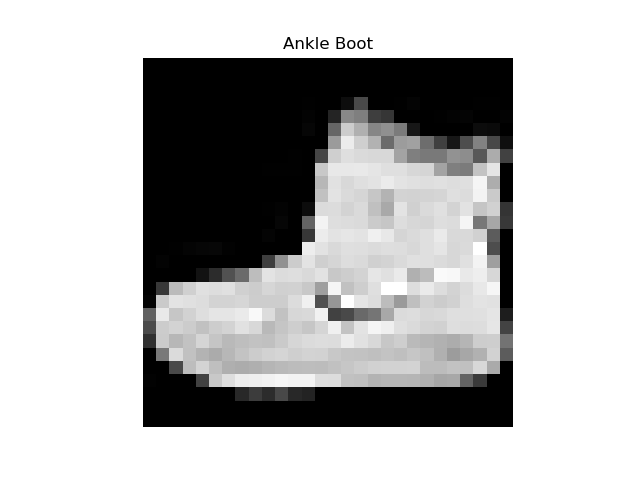
\includegraphics[scale=0.4]{Images/PyTorch/fashion.png}
    \caption{Data point from FashionMNIST}
    \label{fig:fashionmnist_data}
\end{figure}

Now that we have loaded our dataset, we can retrieve our features and labels one sample at a time. However, while training a model, we typically want to pass the samples in minibatches (e.g. in SGD), reshuffle the data at every epoch to reduce model overfitting, and use Python's multiprocessing to speed up data retrieval. We can do all this with the $\texttt{DataLoader}$ API. 

\begin{cverbatim}
from torch.utils.data import DataLoader

train_dataloader = DataLoader(training_data,    # our dataset
                              batch_size=64,    # batch size
                              shuffle=True      # shuffling the data
                            )
test_dataloader = DataLoader(test_data, batch_size=64, shuffle=True)

train_features, train_labels = next(iter(train_dataloader))
print(f"Feature batch shape: {train_features.size()}")
print(f"Labels batch shape: {train_labels.size()}")

# Feature batch shape: torch.Size([64, 1, 28, 28])
# Labels batch shape: torch.Size([64])
\end{cverbatim}

Like in machine learning, we would like to normalize our data in some way. Fortunately, when loading the data, this is automatically done for us. The Fashion image are in PIL format, and the labels are just integers. 
\begin{cverbatim}
from torchvision.transforms import ToTensor, Lambda

ds = datasets.FashionMNIST(
    root="data",
    train=True,
    download=True,
    transform=ToTensor(),
    target_transform=Lambda(lambda y: torch.zeros(10, dtype=torch.float).scatter_(0, 
        torch.tensor(y), value=1))
)
\end{cverbatim}
\begin{enumerate}
    \item $\texttt{transform=ToTensor()}$ tells us to take the images, convert them to a tensor, covert all the elements to floats, and normalize them. 
    \item $\texttt{target\_transform}$ tells us to one-hot encode the integer labels to vectors. It first creates a zero tensor of size 10 (the number of labels in our dataset) and calls $\texttt{scatter\_}$ which assigns a $\texttt{value=1}$ on the index as given by the label y.
\end{enumerate}

\subsubsection{Building a Neural Net}

We can build a neural net as a subclass of $\texttt{nn.Module}$. Note that the $\texttt{nn.flatten}$ method flattens the tensor with $\texttt{start\_dim}$ set to $1$ by default to avoid flattening the first axis (usually the batch axis). 

\begin{cverbatim}
from torch import nn

class NeuralNetwork(nn.Module):
    def __init__(self):
        super().__init__()
        self.flatten = nn.Flatten()
        self.linear_relu_stack = nn.Sequential(
            nn.Linear(28*28, 512),
            nn.ReLU(),
            nn.Linear(512, 512),
            nn.ReLU(),
            nn.Linear(512, 10),
        )

    def forward(self, x):
        x = self.flatten(x)
        logits = self.linear_relu_stack(x)
        return logits
\end{cverbatim}
All of these methods can be used separately, and they can be combined using sequential to form a composition of functions. 
\begin{cverbatim}
X = torch.rand(3, 28, 28)
Y = torch.rand(3, 8)

flatten = nn.Flatten()      # flattens from dim=1 
linear = nn.Linear(8, 4)    # linear map 
relu = nn.ReLU()            # ReLU map 
softmax = nn.Softmax(dim=1) # Softmax map 

print(flatten(X).size())    # torch.Size([3, 784])
print(linear(Y).size())     # torch.Size([3, 4])
print(relu(Y).size())       # torch.Size([3, 8])
print(softmax(Y).size())    # torch.Size([3, 8])
\end{cverbatim}

Next, we want to create an instance of this neural network and move it to our cuda device. 
\begin{cverbatim}
model = NeuralNetwork().to(device)
print(model)

# NeuralNetwork(
#   (flatten): Flatten(start_dim=1, end_dim=-1)
#   (linear_relu_stack): Sequential(
#     (0): Linear(in_features=784, out_features=512, bias=True)
#     (1): ReLU()
#     (2): Linear(in_features=512, out_features=512, bias=True)
#     (3): ReLU()
#     (4): Linear(in_features=512, out_features=10, bias=True)
#   )
# )
\end{cverbatim}

To use the model, we can just directly pass in the input data, which executes the model's forward propagation ($\texttt{forward}$ method). Do not call $\texttt{model.forward()}$ directly! 
\begin{cverbatim}
X = torch.rand(3, 28, 28, device=device)
logits = model(X)
pred_probab = nn.Softmax(dim=1)(logits)
y_pred = pred_probab.argmax(1)
print(f"Predicted class: {y_pred}")

# tensor([[-0.0518,  0.0379, -0.0579,  0.0050,  0.0367,  0.0958,  0.0055,  0.1385,
#           0.0464, -0.0017]], device='cuda:0', grad_fn=<AddmmBackward0>)
# tensor([[0.0924, 0.1011, 0.0919, 0.0978, 0.1010, 0.1071, 0.0979, 0.1118, 0.1019,
#          0.0972]], device='cuda:0', grad_fn=<SoftmaxBackward0>)
# Predicted class: tensor([7], device='cuda:0')
\end{cverbatim}

We can also access parameters by calling $\texttt{model.named\_parameters()}$, which gives us a list of tuples $(name, param)$, where name is simply the name of the weight, and the param is the matrix representing the linear mapping or the bias term. 
\begin{cverbatim}
for name, param in model.named_parameters():
    print(f"Layer: {name} | Size: {param.size()} | Values : {param[:2]} \n")
\end{cverbatim}

\subsubsection{Automatic Differentiation}

The forward and backward API for a computational gate multiplying its inputs 
\begin{center}
\begin{tikzpicture}[scale=1.5, every node/.style={draw, circle, minimum size=1cm}]

  % Input nodes
  \node (x) at (0, 1) {$x$};
  \node (y) at (0, -1) {$y$};

  % Multiply gate node
  \node[shape=rectangle] (multiply) at (1.5, 0) {$\times$};

  % Output node
  \node (z) at (3.5, 0) {$z$};

  % Connections
  \draw[->] (x) -- (multiply);
  \draw[->] (y) -- (multiply);
  \draw[->] (multiply) -- (z);

\end{tikzpicture}
\end{center}
is represented with the code below. 
\begin{cverbatim}
class MultiplyGate(object): 
    def forward(x, y): 
        z = x * y 
        self.x = x      # must keep these around! 
        self.y = y 
        return z 

    def backward(dz): 
        dx = self.y * dz  
        dy = self.x * dz 
        return [dx, dy] 
\end{cverbatim}


\subsubsection{Optimizing Model Parameters}

Bsaically in each epoch, we want to do two things: 
\begin{enumerate}
    \item \textit{Train Loop}: Iterate over the (minibatch) training dataset and try to converge to optimal parameters using backprop. 
    \item \textbf{Test Loop}: Iterate over the test dataset to check if model performance is improving. 
\end{enumerate}

Once we compute the gradient of a given loss function, we can use different optimizers like SGD or ADAM to optimize. 
\begin{cverbatim}
loss_fn = nn.CrossEntropyLoss()
optimizer = torch.optim.SGD(
    model.parameters(),     # which parameters to optimize
    lr=1e-3                 # learning rate 
)
\end{cverbatim}
Our train loop 
\begin{cverbatim}
def train(dataloader, model, loss_fn, optimizer):
    size = len(dataloader.dataset)
    model.train()
    for batch, (X, y) in enumerate(dataloader):
        X, y = X.to(device), y.to(device)

        # Compute prediction error
        pred = model(X)
        loss = loss_fn(pred, y)

        # Backpropagation
        loss.backward()
        optimizer.step()
        optimizer.zero_grad()

        if batch % 100 == 0:
            loss, current = loss.item(), (batch + 1) * len(X)
            print(f"loss: {loss:>7f}  [{current:>5d}/{size:>5d}]")
\end{cverbatim}
We can then evaluate the model's performance against the test dataset. 
\begin{cverbatim}
def test(dataloader, model, loss_fn):
    size = len(dataloader.dataset)
    num_batches = len(dataloader)
    model.eval()
    test_loss, correct = 0, 0
    with torch.no_grad():
        for X, y in dataloader:
            X, y = X.to(device), y.to(device)
            pred = model(X)
            test_loss += loss_fn(pred, y).item()
            correct += (pred.argmax(1) == y).type(torch.float).sum().item()
    test_loss /= num_batches
    correct /= size
    print(f"Test Error: \n Accuracy: {(100*correct):>0.1f}%, Avg loss: {test_loss:>8f} \n")
\end{cverbatim}
Now we run this through a loop over some number of epochs. 
\begin{cverbatim}
epochs = 5
for t in range(epochs):
    print(f"Epoch {t+1}\n-------------------------------")
    train(train_dataloader, model, loss_fn, optimizer)
    test(test_dataloader, model, loss_fn)
print("Done!")
\end{cverbatim}

\section{Training Stability}

Training stability refers to helping the training process, which does not improve the theoretical upper bound on the accuracy of the neural net, but are extremely important for practical applications. It is related to regularization, which prevents the neural net from overfitting to the data. They are both related as they improve the performance of training and the neural network itself, but it good to distinguish them. Given some loss landscape, regularization ensures that we don't ``fall" into some deep hole that looks great on our training error, but does terribly on our testing error. On the other hand, training stability ensures that we update our parameters efficiently to traverse the landscape. 

\subsection{Weight Initialization}

Now how should we initialize our weights? 
\begin{enumerate}
    \item If we set $\boldsymbol{\theta} = \mathbf{0}$, i.e. set all weights to $0$, then all of our activations are going to be the same, and thus all our gradients will be the same, meaning that are updates will be the same for every weight, which is not good mixing. 
    \item Therefore, the next thing to do is initialize all weights according to small independent Gaussians $N(0, 0.1)$. However, this has problems since for many layer networks, as we multiply our inputs by small values over and over, we will eventually converge to a vector of $0$s for each hidden layer. The activations will go to $0$ and the gradients also $0$, and so there will be no learning. 
    \item If we initialize them as random weights with a large norm, then the activations may saturate (for tanh), meaning that the gradients will be $0$ and there will be no learning. 
\end{enumerate}
Therefore, we can use something called \textbf{Xavier initialization} or \textbf{He initialization}. Proper initialization is an active area of research, and PyTorch will automatically implement the latest initialization for us in our layer constructors. 

\subsection{Optimizers}



\subsection{Vanishing Gradient Problem}

\subsubsection{Activation Functions}

The choice of the activation function can have a significant impact on your training, and we will describe a few examples below. The first thing to note is that we must ensure that there is a nonzero gradient almost everywhere. If, for example, we had a piecewise constant activation function, the gradient is $0$ almost everywhere, and it would kill the gradient of the entire network. 

\begin{example}[Sigmoid]
Sigmoid activations are historically popular since they have a nice interpretation as a saturating ``fire rate" of a neuron. However, there are 3 problems: 
\begin{enumerate}
    \item The saturated neurons ``kill" the gradients, since if the input at any one point in the layers is too positive or negative, the gradient will vanish, making very small updates. This is known as the \textbf{vanishing gradient problem}. Therefore, the more layers a neural network has, the more likely we are to see this vanishing gradient problem. 
    \item Sigmoid functions are not zero centered (i.e. its graph doesn't cross the point $(0, 0)$ ). Consider what happens when the input $x$ to a neuron is always positive. Then, the sigmoid $f$ will have a gradient of 
    \[f \bigg( \sum_i w_i x_i + b \bigg) \implies \frac{\partial f}{\partial w_i} = f^\prime \bigg( \sum_i w_i x_i + b \bigg) 
    \, x_i\]
    which means that the gradients $\nabla_\mathbf{w} f$ will always have all positive elements or all negative elements, meaning that we will be restricted to moving in certain nonoptimal directions when updating our parameters. 
\end{enumerate}
\end{example}

\begin{example}[Hyperbolic Tangent]
The hyperbolic tangent is zero centered, which is nice, but it still squashes numbers to range $[-1, 1]$ and therefore kills the gradients when saturated. 
\end{example}

\begin{example}[Rectified Linear Unit]
The ReLU function has the following properties: 
\begin{enumerate}
    \item It does not saturate in the positive region. 
    \item It is very computationally efficient (and the fact that it is nondifferentiable at one point doesn't really affect computations). 
    \item It converges much faster than sigmoid/tanh in practice. 
    \item However, note that if the input is less than $0$, then the gradient of the ReLU is $0$. Therefore, if we input a vector that happens to have all negative values, then the gradient would vanish and we wouldn't make any updates. These ReLU ``dead zones" can be a problem since it will never activate and never update, which can happen if we have bad initialization. A more common case is when your learning rate is too high, and the weights will jump off the data manifold. 
\end{enumerate}
\end{example}

\begin{example}[Leaky ReLU]
The leaky ReLU 
\[\sigma(x) = \max\{0.01 x, x\}\]
does not saturate (i.e. gradient will not die), is computationally efficient, and converges much faster than sigmoid/tanh in practice. We can also parameterize it with $\alpha$ and have the neural net optimize $\alpha$ along with the weights. 
\[\sigma(x) = \max\{\alpha x, x\}\]
\end{example}

\begin{example}[Exponential Linear Unit]
The exponential linear unit has all the benefits of ReLU, with closer to mean outputs. It has a negative saturation regime compared with leaky ReLU, but it adds some robustness to noise. 
\[\sigma(x) = \begin{cases} x & \text{ if } x > 0 \\ \alpha \big(\exp{x} - 1 \big) & \text{ if } x \leq 0 \end{cases}\]
\end{example}

\begin{example}[Max-Out Neuron]
The maxout neuron has the following form 
\[\sigma(\mathbf{x}) = \max\{ \mathbf{w}_1^T \mathbf{x} + b_1 , \mathbf{w}_2^T \mathbf{x} + b_2 \}\]
This generalizes the ReLU and leaky ReLU. It is linear, which is nice, and it does not saturate, meaning that the gradient will never die. However, this doubles the number of parameters in the neuron, making it more computationally expensive. 
\end{example}

In practice, we should do the following: 
\begin{enumerate}
    \item Use ReLU and be careful with your learning rates. 
    \item Try out leaky ReLU, maxout, and ELU 
    \item Try out tanh but don't expect much 
    \item Do not use sigmoid, since it is obsolete
\end{enumerate}

\subsubsection{Residual Connections}


\begin{center}
    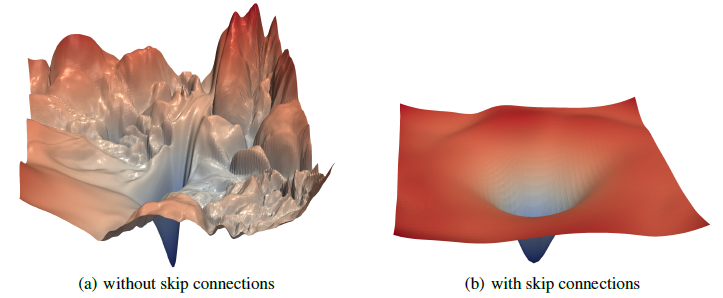
\includegraphics[scale=0.3]{Images/resnet_loss.png}
\end{center}


Some residual architecture solutions include feedforward/convolutional architectures that add more direct connections from the lower layers, thus allowing the gradient to flow. 
\begin{enumerate}
    \item The \textbf{ResNet} (\textbf{Residual Connections}) includes an additional path from layer $i$ to layer $j$ that skips the intermediate layers and simply goes through an identity connection, which is then summed with the original path during forward prop. 
    \begin{center}
        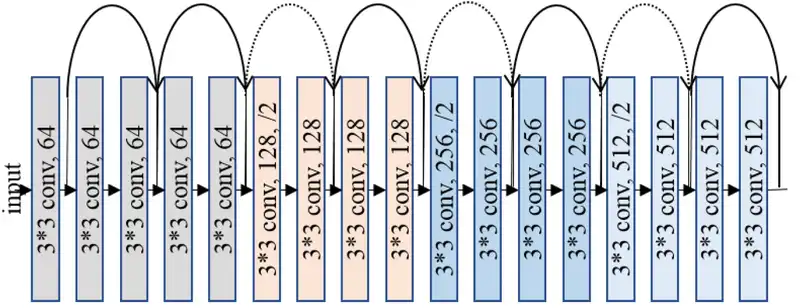
\includegraphics[scale=0.3]{Images/resnet-arch.png}
    \end{center}
    
    \item The \textbf{DenseNet} directly connects each layer to all future layers, which allows for maximal flow but a lot of computational cost. 
    \begin{center}
        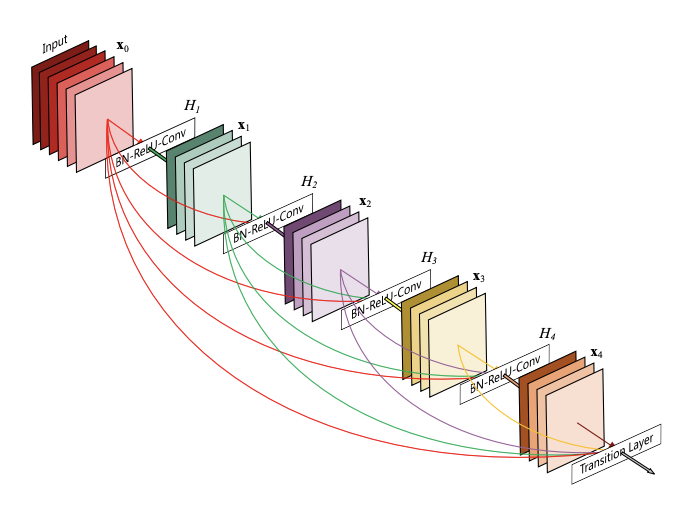
\includegraphics[scale=0.5]{Images/densenet.png}
    \end{center}

    \item The \textbf{HighwayNet} (\textbf{Highway Connections}) is similar to residual connections, but the identity connection vs the transformation layer is controlled by a dynamic gate. These are inspired by LSTMs, but are applied to deep feedforward/convolutional networks. 
\end{enumerate}


\subsection{Exploding Gradient Problem}

\subsubsection{Normalization Layers}
Note that given the distribution of the covariates $X$ in $\mathcal{X} \subset \mathbb{R}^D$, our neural network transforms them into different distributions in $\mathbb{R}^{[l]}$. For example, in the first layer, where both the affine and the activation functions are usually measurable, the random variable 
\[\boldsymbol{\sigma} \big( \mathbf{W}^{[1]} X + \mathbf{b}^{[1]} \big)\]
will induce a probability measure over $\mathbb{R}^{[1]}$. This phenomenon where the distribution of each layer's inputs change is called \textbf{internal covariate shift}. 

It has long been known that standardization of the inputs (i.e. transforming them to have $0$ mean and unit variance) results in better convergence of the neural net, and extending this to hidden layers, it would be advantageous to achieve the same standardization of each layer. In one case, if our inputs to a saturated activation (like tanh, which are saturated for very positive or very negative inputs) are too big, then the gradient will die off, which is why we want to constrain them to a small interval around $0$. This is called a \textbf{normalization layer}, which works like this: 
\begin{enumerate}
    \item We select a minibatch of training examples $\mathcal{B} = \{\mathbf{x}^{(1)}, \ldots, \mathbf{x}^{(B)}\}$. Ideally, we would get the mean and variance over the whole batch, but in SGD, the minibatch is a good approximation of the distribution, so we take it with respec to $\mathcal{B}$. 
    
    \item We standardize the $\mathbf{x}^{(b)}$'s element-wise. That is, for a given feature dimension $d$, 
    \[\mu_d = \frac{1}{B} \sum_b x^{(b)}_d, \;\; \sigma^2_d = \frac{1}{B} \sum_{b} \big(x^{(b)}_d - \mu_d \big)^2\]
    and we set 
    \[\hat{x}_d^{(b)} = \frac{x_d^{(b)} - \mu_d}{\sqrt{\sigma^2_d + \epsilon}}, \;\; \text{ i.e. } \hat{\mathbf{x}}^{(b)} = (\mathbf{x}^{(b)} - \boldsymbol{\mu}) \odot (\boldsymbol{\sigma}^2 + \boldsymbol{\epsilon})^{-1/2}\]
    where $\epsilon$ is a small float needed for numerical stability. 
    This element-wise normalization is not optimal if the covariates are correlated, but in practicality this is not too big of a problem. 

    \item However, constraining our normalization to the unit Gaussian in many cases constrains us to the linear regime of the nonlinearity of our activation functions (e.g. sigmoid or tanh). We would like a little bit of control over how much saturation we would like to have, so we allow some rescaling and reshifting (element-wise, again) parameters for flexibility. 
    \[\mathbf{y} = \boldsymbol{\gamma} \odot \hat{\mathbf{x}} + \boldsymbol{\beta} = \mathrm{BN}_{\boldsymbol{\gamma}, \boldsymbol{\beta}} (\mathbf{x})\]
    If the network learns that $\gamma_d = \sqrt{\Var(x_d)}$ and $\beta_d = \mathbb{E}[x_d]$, then it is as if there was no normalization at all, just the identity mapping. If $\mathbf{x} \in \mathbb{R}^n$, then this one normalization layer gives us $2n$ more parameters to learn in our network. 
\end{enumerate}
Therefore, rather than our steps being simply 
\[\mathbf{z}^{[l]} \mapsto \boldsymbol{\sigma}(\mathbf{z}^{[l]}) = \mathbf{a}^{[l]}\]
we now have the normalization later 
\[\mathbf{z}^{[l]} \mapsto \boldsymbol{\sigma}\big( \mathrm{BN}_{\boldsymbol{\gamma}, \boldsymbol{\beta}})(\mathbf{z}^{[l]}) \big) = \mathbf{a}^{[l]}\]
In test time, we have the trained parameters, along with the $\boldsymbol{\gamma}$'s and $\boldsymbol{\beta}$'s, but we now recompute the normalization constants with respect to the entire training set, not a minibatch. 

\subsubsection{Max Norm Regularization}

Though large momentum and learning rate speed up learning, they sometimes cause the network weights to grow very large. To prevent this, we can use max-norm regularization. This constraints the norm of the vector of incoming weights at each hidden unit to be bound by a constant $c$. Typical values of $c$ range from $3$ to $4$. 


\section{Regularization}

\subsection{Early Stopping}

\subsection{L1 and L2 Regularization}

\subsection{Dropout}

Overfitting is always a problem. With unlimited computation, the best way to regularize a fixed-sized mdoel is to average the predictions of all possible settings of the parameters, weighting each setting by its posterior probability given the training the data. However, this is computationally expensive and cannot be done for moderately complex models. 

The dropout method addresses this issue. We literally drop out some features (not the weights!) before feeding them to the next layer by setting some activation functions to $0$. Given a neural net of $N$ total nodes, we can think of the set of its $2^N$ thinned subnetworks. For each training minibatch, a new thinned network is sampled and trained. 

At each layer, recall that forward prop is basically 
\begin{align*}
    \mathbf{z}^{[l+1]} & = \mathbf{W}^{[l+1]} \mathbf{a}^{[l]} + \mathbf{b}^{[l+1]} \\
    \mathbf{a}^{[l+1]} & = \boldsymbol{\sigma} (\mathbf{z}^{[l+1]}) 
\end{align*}
Now what we do with dropout is 
\begin{align*}
    r_j^{[l]} & \sim \mathrm{Bernoulli}(p) \\
    \Tilde{\mathbf{a}}^{[l]} & = \mathbf{r}^{[l]} \odot \mathbf{a}^{[l]} \\
    \mathbf{z}^{[l+1]} & = \mathbf{W}^{[l+1]} \Tilde{\mathbf{a}}^{[l]} + \mathbf{b}^{[l+1]} \\
    \mathbf{a}^{[l+1]} & = \boldsymbol{\sigma} (\mathbf{z}^{[l+1]}) 
\end{align*}
Basically we a sample a vector of $0$s and $1$s from a multivariate Bernoulli distribtion. We element-wise multiply it with $\mathbf{a}^{[l]}$ to create the thinned output $\Tilde{\mathbf{a}}^{[l]}$. In test time, we do not want the stochasticity of having to set some activation functions to $0$. That is, consider the neuron $\mathbf{a}^{[l]}$ and the random variable $\Tilde{\mathbf{a}}^{[l]}$. The expected value of $\mathbf{z}^{[l+1]}$ is 
\[\mathbb{E}[\mathbf{z}^{[l+1]}] = \mathbb{E}[ \mathbf{W}^{[l+1]} \Tilde{\mathbf{a}}^{[l]} + \mathbf{b}^{[l+1]}] = \mathbb{E}[ \mathbf{W}^{[l+1]} \Tilde{\mathbf{a}}^{[l]}] = p \mathbb{E}[\mathbf{W}^{[l+1]} \mathbf{a}^{[l]}] \]
and to make sure that the output at test time is the same as the expected output at training time, we want to multiply the weights by $p$: $W^{[l]}_{\text{test}} = p \, W^{[l]}_{\text{train}}$. Another way is to use \textbf{inverted dropout}, where we can divide by $p$ in the training stage and keep the testing method the same. 

In PyTorch, this can be done with the dropout function, where $\texttt{p}$ represents the probability of an element getting dropped out and $\texttt{inplace=True}$ means that the operation will be done in place (i.e. the variable itself will be changed). We should set it to false since we don't want to set all the parameters to $0$ permanently. 
\begin{cverbatim}
drop = nn.Dropout(p=0.5, inplace=False)
X = torch.rand(4) 
print(X)            # tensor([0.3342, 0.8208, 0.3765, 0.1820])
print(drop(X))      # tensor([0.6684, 1.6417, 0.0000, 0.0000])
print(X)            # tensor([0.3342, 0.8208, 0.3765, 0.1820])
\end{cverbatim}

\begin{cverbatim}
class NeuralNetwork(nn.Module):
    def __init__(self):
        super().__init__()
        self.flatten = nn.Flatten()
        self.linear_relu_stack = nn.Sequential(
            nn.Linear(28*28, 512),
            nn.ReLU(),
            nn.Dropout(p=0.5, inplace=False), 
            nn.Linear(512, 512),
            nn.ReLU(),
            nn.Dropout(p=0.5, inplace=False), 
            nn.Linear(512, 10)
        )

    def forward(self, x):
        x = self.flatten(x)
        logits = self.linear_relu_stack(x)
        return logits
\end{cverbatim}

When you call $\texttt{model.eval()}$, PyTorch automatically turns off Dropout (as well as other functionalities such as BatchNorm). Similarly, when you call $\texttt{model.train()}$, Dropout is turned on and will be used during training. It is expected that a dropout network with $M$ hidden units in each layer will have $pM$ units after dropout. Therefore, if an $M$-sized layer is optimal for a standard neural net on any given task, then a good dropout net should have at least $M/p$ units. 


\subsection{Data Augmentation}

It is well known that having more training data helps with overfitting, and so we may be able to perform basic transformations to our current data to artificially generate more training data. For example, if we have images, then we can flip, crop, translate, rotate, stretch, shear, and lens-distort these images with the same label. 


\subsection{Network Pruning}

It can be computationally and memory intensive to train and utilize neural networks. This is where network pruning comes in, which attempts to identify a subnetwork that performs as well as the original. Given a neural net $f(\mathbf{x}, \boldsymbol{\theta})$ where $\boldsymbol{\theta} \in \mathbb{R}^M$, a pruned neural network can be thought of as a subnetwork $f(\mathbf{x}, \mathbf{m} \odot \boldsymbol{\theta})$, where $\mathbf{m}$ is a \textbf{mask}, i.e. a vector in $\{0, 1\}^M$ that, when multiplied component-wise to $\boldsymbol{\theta}$, essentially ``deletes" a portion of the parameters. 
\begin{center}
    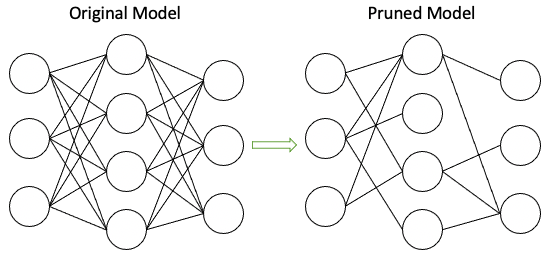
\includegraphics[scale=0.4]{Images/pruned_network.png}
\end{center}
This idea has been around for a long time, and the general method of pruning is as such: 
\begin{enumerate}
    \item We initialize the neural network $f(\mathbf{x}, \boldsymbol{\theta}_0)$ and train it until we have $f(\mathbf{x}, \boldsymbol{\theta})$. 
    \item We now prune the network. The most basic pruning scheme is to keep the top $k\%$ largest weights, since smaller weights do not contribute much to the forward prop, and thus can be ignored. 
\end{enumerate}
These pruned networks have been shown to reach accuracies as high as the original network, with equal training progress. Now, if we were to take only this pruned network and train it from the beginning, it will perform as well as the original network, \textit{only under} the condition that we start from the same initialization $\mathbf{m} \odot \boldsymbol{\theta}$. If we take this subnetwork and initialize it differently at $\boldsymbol{\theta}_0^\prime$, then this subnetwork would not train well. Therefore, the performance of the pruned network is dependent on the initialization! 

If we had initialized the full network differently, trained it, and then pruned again, we may have a different subnetwork that will only train well on its own given this new initialization. Therefore, a good initialization is extremely important for training subnetworks. This fact doesn't help much since we can't just take some arbitrary subnetwork and train it since we don't know the good initialization. We must always train the full network, then find the subnetwork, and then find its initialization. 

This is essentially the \textbf{lottery ticket hypothesis}, which states that a randomly-initialized, dense neural network contains a subnetwork that is initialized such that, when trained in isolation, it can match the test accuracy of the original network after training for at must the same number of iterations. 

This paper hints at why neural networks work at all. It first states that only a very small subnetwork is responsible for the vast majority of its performance, but it must be initialized at the right position. But by overparameterizing these neural nets so much (by a certain margin), they have so many different combinations of subnetworks such that whatever initialization you throw at it, it is guaranteed that some subnetwork within it will train well with this initialization. This subnetwork is called the \textit{winning ticket}. 

\subsection{Summary}

Here is a few steps you can take as a guide to training a neural network. 
\begin{enumerate}
    \item Preprocess the data. 
    \item Choose your neural net architecture (number of layers/neurons, etc.) 
    \item Do a forward pass with the initial parameters, which should be small, and check that the loss is reasonable (e.g. $\log(1/10) \approx 2.3$ for softmax classification of 10 classes). 
    \item Now crank up the regularization term, and your loss should have gone up. 
    \item Now try to train on only a very small portion of your data without regularization using SGD, which you should be able to overfit and get the accuracy to 100\%. 
    \item Now you can train your whole dataset. Start off with a small regularization (e.g. 1e-6) and find a learning rate that makes the loss go down. 
    \begin{enumerate}
        \item Run for a few epochs to see if the cost goes down too slowly (step size is too small) or the cost explodes (step size too big). A general tip is that if the cost is ever bigger than $3$ times the original cost, then this is an indication that the cost has exploded. 
        \item We can run a grid search (in log space) over the learning rate and the regularization hyperparameters over say 10 epochs each, and compare which one makes the most progress. 
    \end{enumerate}
    \item Monitor and visualize the loss curve. 
    \begin{center}
        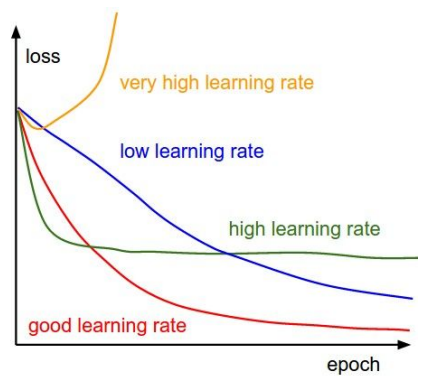
\includegraphics[scale=0.5]{Images/loss_curve.png}
    \end{center}
    If you see loss curves that are flat for a while and then start decreasing, then bad initialization is a prime suspect. 
    \item We also want to track the ratio of weight updates and weight magnitudes. That is, we can take the norm of the weights $\boldsymbol{\theta}$ and the gradient updates $\nabla \boldsymbol{\theta}$, and a rule of thumb is that the ratio should be about 
    \[\frac{||\nabla \boldsymbol{\theta}||}{||\boldsymbol{\theta}||} \approx 0.001 \text{ or } 0.01\]
\end{enumerate}



\section{Convolutional Neural Networks}

\subsection{Kernels}

A convolution is described by a \textbf{kernel}, also called a \textbf{filter}, which is simply a $K \times K$ matrix. It does not have to be square but is conventionally so. It goes through a grayscale image at every point and compute the dot product of the kernel with the overlapping portion of the image, creating a new pixel. This can be shown in Figure \ref{fig:convolution}. 

\begin{figure}
\centering
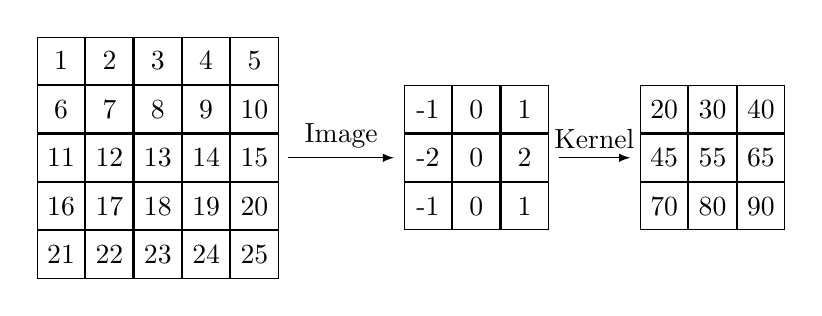
\begin{tikzpicture}[>=latex]

% Image
\matrix[matrix of nodes, nodes={draw, minimum size=0.6cm, anchor=center}] (image) {
    1 & 2 & 3 & 4 & 5 \\
    6 & 7 & 8 & 9 & 10 \\
    11 & 12 & 13 & 14 & 15 \\
    16 & 17 & 18 & 19 & 20 \\
    21 & 22 & 23 & 24 & 25 \\
};

% Kernel
\matrix[matrix of nodes, nodes={draw, minimum size=0.6cm, anchor=center}, right=3cm] (kernel) {
    -1 & 0 & 1 \\
    -2 & 0 & 2 \\
    -1 & 0 & 1 \\
};

% Convolution result
\matrix[matrix of nodes, nodes={draw, minimum size=0.6cm, anchor=center}, right=6cm] (result) {
    20 & 30 & 40 \\
    45 & 55 & 65 \\
    70 & 80 & 90 \\
};

% Arrows
\draw[->] (image) -- node[midway, above] {Image} (kernel);
\draw[->] (kernel) -- node[midway, above] {Kernel} (result);

\end{tikzpicture}
\caption{Convolution using a kernel on an image.}
\label{fig:convolution}
\end{figure}

Now if this was a color image, then the $K \times K$ kernel $\mathcal{K}$ would dot over all 3 layers, without changing over all 3 layers. This is equivalent to applying the kernel over all 3 channels separately, and then combining them together into one. Another thing to note is that the output image of a kernel would be slightly smaller than the input image, since the kernel cannot go over the edge. However, there are padding schemes to preserve the original dimensions. To construct our custom kernel, we can simply create a custom matrix: 
\begin{cverbatim}
img = cv2.imread("cats.jpg")

# create custom 5x5 kernel
kernel = (1/25) * np.ones((5, 5), dtype=np.float32)

# apply to image
dst = cv2.filter2D(img, -1, kernel)
cv2.imshow("Park", dst)
cv2.waitKey(0)
\end{cverbatim}
Note that the kernel matrix may have the property that all of its entries sum to $1$, meaning that on average, the expected value of the brightness of each pixel will be $0$, and the values will be left unchanged on average. However, this is not a requirement. 

\begin{example}[Mean Blur, Gaussian Blur]
The mean and Gaussian blur is defined with kernels that are distributed uniformly and normally across the entire matrix. You can see how this would blur an image since for every pixel, we take the weighted average over all of its surrounding pixels. 
\[\text{mean} = \frac{1}{25} \begin{bmatrix} 1 & 1 & 1 & 1 & 1 \\ 1 & 1 & 1 & 1 & 1 \\ 1 & 1 & 1 & 1 & 1 \\ 1 & 1 & 1 & 1 & 1 \\ 1 & 1 & 1 & 1 & 1 \end{bmatrix}, \;\;\;\;\; \text{Gaussian} = \frac{1}{273} \begin{bmatrix} 1 & 4 & 7 & 4 & 1 \\ 4 & 16 & 26 & 16 & 4 \\ 7 & 26 & 41 & 26 & 7 \\ 4 & 16 & 26 & 16 & 4 \\ 1 & 4 & 7 & 4 & 1 \end{bmatrix}\]
On a large scale, there really aren't any discernable differences, as seen in Figure \ref{fig:blur}, but the Guassian blur is known to be a more realistic representation of how humans receive blur. 
\begin{figure}[hbt!]
    \centering
    \begin{subfigure}[b]{0.32\textwidth}
    \centering
        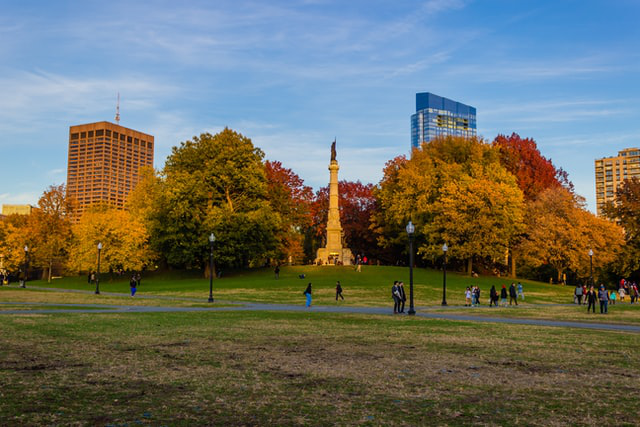
\includegraphics[width=\textwidth]{Images/OpenCV/Park_Full.png}
        \caption{Original image. }
        \label{fig:original_image}
    \end{subfigure}
    \begin{subfigure}[b]{0.32\textwidth}
    \centering
        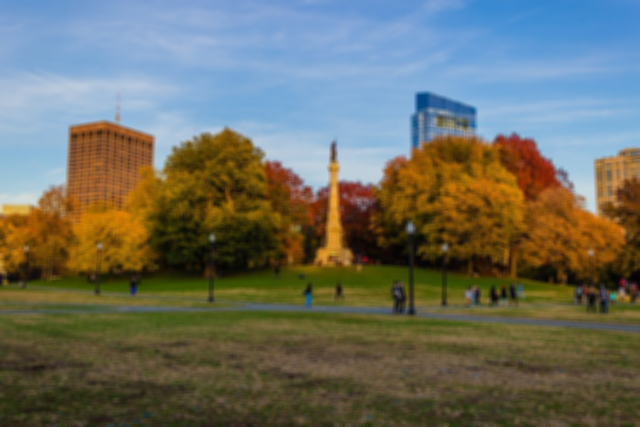
\includegraphics[width=\textwidth]{Images/OpenCV/Mean_Blur.png}
        \caption{$5 \times 5$ mean blur applied. }
        \label{fig:mean_blur_image}
    \end{subfigure}
    \begin{subfigure}[b]{0.32\textwidth}
    \centering
        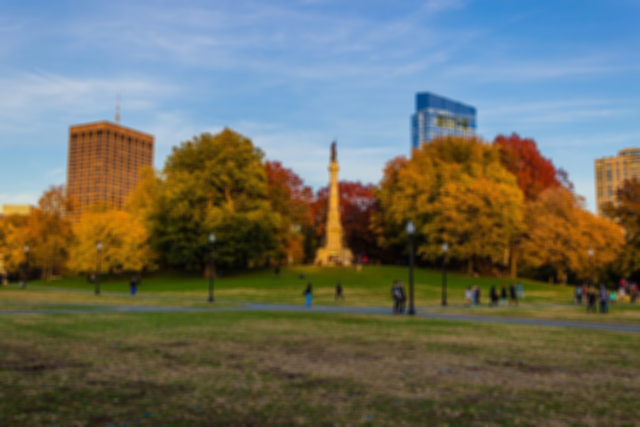
\includegraphics[width=\textwidth]{Images/OpenCV/Gaussian_Blur.png}
        \caption{$5 \times 5$ Gaussian blur applied. }
        \label{fig:normal_blur_image}
    \end{subfigure}

    \caption{Comparison of blurring kernels on image. }
    \label{fig:blur}
\end{figure}
\end{example}

\begin{example}[Sharpening]
A sharpening of an image would be the opposite of a blur, meaning that we emphasize the center pixel and reduce the surrounding pixels. 
\[\text{Sharpen} = \begin{bmatrix} 0 & -1 & 0 \\ -1 & 5 & -1 \\ 0 & -1 & 0 \end{bmatrix}\]
\begin{figure}[hbt!]
    \centering
    \begin{subfigure}[b]{0.45\textwidth}
    \centering
        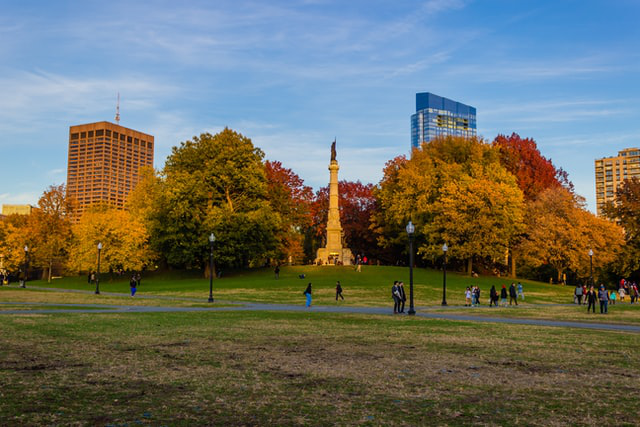
\includegraphics[width=\textwidth]{Images/OpenCV/Park_Full.png}
        \caption{Original image. }
        \label{fig:original_image_2}
    \end{subfigure}
    \begin{subfigure}[b]{0.45\textwidth}
    \centering
        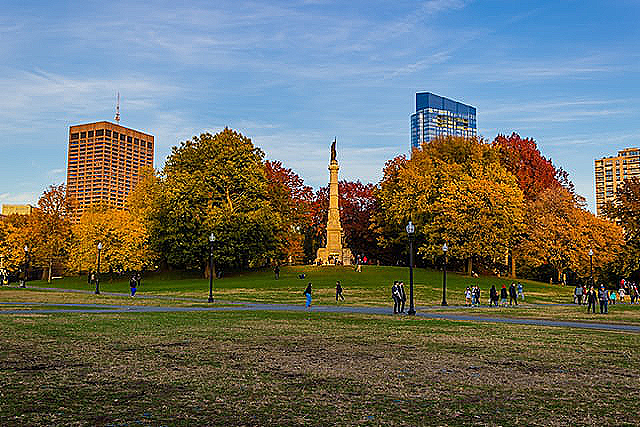
\includegraphics[width=\textwidth]{Images/OpenCV/Sharpen.png}
        \caption{$3 \times 3$ sharpening applied. }
        \label{fig:sharpened_image}
    \end{subfigure}

    \label{fig:sharpen}
    \caption{Sharpening kernels applied to image. }
\end{figure}
\end{example}

\begin{example}[Edge Detection]
The edge detecting kernel looks like the following, which differs for horizontal and vertical edge detection. Note that the sum of all of its values equal $0$, which means that for areas that have a relatively constant value of pixels, all the surrounding ones will ``cancel" out and the kernel will output a value of $0$, corresponding to black. This is why we see mostly black in the photo. 
\[\text{Horizontal} = \begin{bmatrix} -1 & 0 & 1 \\ -2 & 0 & 2 \\ -1 & 0 & 1 \end{bmatrix}, \;\;\;\;\;\; \text{Vertical} = \begin{bmatrix} -1 & -2 & -1 \\ 0 & 0 & 0 \\ 1 & 2 & 1 \end{bmatrix}\]
\begin{figure}[hbt!]
    \centering
    \begin{subfigure}[b]{0.45\textwidth}
    \centering
        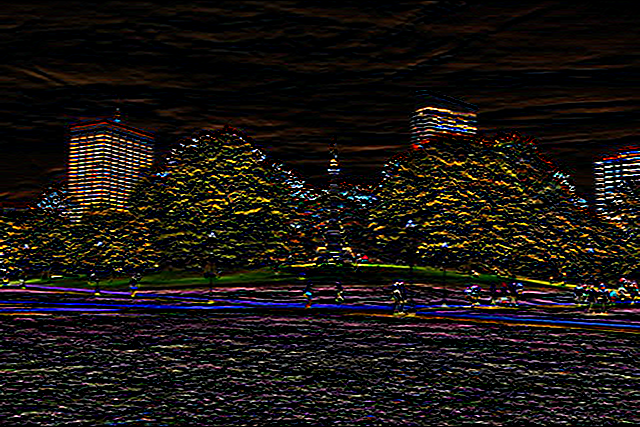
\includegraphics[width=\textwidth]{Images/OpenCV/Horizontal.png}
        \caption{$3 \times 3$ horizontal edge detecting kernel applied. }
        \label{fig:horizontal_edge}
    \end{subfigure}
    \begin{subfigure}[b]{0.45\textwidth}
    \centering
        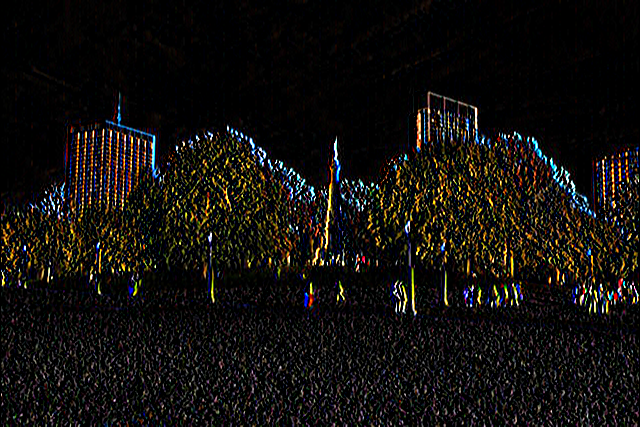
\includegraphics[width=\textwidth]{Images/OpenCV/Vertical.png}
        \caption{$3 \times 3$ vertical edge detecting kernel applied. }
        \label{fig:vertical_edge}
    \end{subfigure}

    \label{fig:edge_detection}
    \caption{Edge detecting kernels applied to image. }
\end{figure}
\end{example}

Just to explicitly see what is actually computed, let's do one computational example. 

\begin{example} 
    Consider an RGB iamge $X = [X_0, X_1, X_2]$ with three channels, and given as follows 
    \[X_0 = \begin{bmatrix} 2 & 1 & 0 & 0 \\ 0 & 0 & 2 & 1 \\ 0 & 2 & 0 & 1 \\ 2 & 1 & 0 & 1 \end{bmatrix}, \;\; X_1 = \begin{bmatrix} 2 & 2 & 0 & 0 \\ 0 & 0 & 2 & 1 \\ 0 & 0 & 2 & 0 \\ 0 & 1 & 0 & 1 \end{bmatrix}, \;\; X_2 = \begin{bmatrix} 2 & 1 & 0 & 0 \\ 0 & 0 & 2 & 1 \\ 2 & 0 & 0 & 0 \\ 0 & 1 & 0 & 1 \end{bmatrix}\]
    The image is passed through the convolutional filter with the weights $W = [W_0, W_1, W_2] \in \mathbb{R}^{3 \times 3 \times 3}$ and step size $1$, and given as follows 
    \[W_0 = \begin{bmatrix} 1 & 0 & 0 \\ 0 & -2 & 0 \\ 0 & 0 & -1 \end{bmatrix}, \;\; W_1 = \begin{bmatrix} 1 & 2 & 0 \\ 2 & 0 & - 1 \\ 0 & -1 & 1 \end{bmatrix}, \;\; W_2 = \begin{bmatrix} 0 & 0 & -2 \\ 0 & 1 & 2 \\ -2 & 2 & 0 \end{bmatrix} \]
The output of the convolutional filter is given as 
\[Y = \mathrm{ReLU} \bigg( \sum_{i=0}^2 (X_i^\prime \ast W_i) + 2 \cdot 1_{4 \times 4}\bigg)\]
where $Y$ is the output image, $X^\prime$ is the input image after applying $0$ padding around the edges, and $\ast$ is the discrete convolution operator. Compute the output $Y$, and then apply max pooling on nonoverlapping $2 \times 2$ submatrices, and then apply average pooling on non-overlapping $2 \times 2$ submatrices. 
\end{example}
\begin{solution}
We can compute 
\begin{align*} 
    X_0 \ast  W_0 & = \begin{bmatrix} -4 & -4 & -1 & 0 \\ -2 & 2 & -4 & -2 \\ -1 & -4 & -1 & 0 \\ -4 & -2 & 2 & -2 \end{bmatrix} \\
    X_1 \ast W_1 & = \begin{bmatrix} -2 & 6 & 3 & -1 \\ 4 & 6 & -1 & 4 \\ 1 & -3 & 5 & 7 \\ -1 & 0 & 5 & 2 \end{bmatrix} \\
    X_2 \ast W_2 & = \begin{bmatrix} 4 & 1 & 4 & -2 \\ 2 & 0 & 4 & 11 \\ 2 & -2 & -4 & 2 \\ 2 & 1 & 2 & 1 \end{bmatrix}
\end{align*}
and so we get 
\[Y = \begin{bmatrix} 0 & 5 & 8 & 0 \\ 6 & 10 & 1 & 5 \\ 4 &  0 & 2 & 11 \\ 0 & 1 & 11 & 3 \end{bmatrix}\]
Maxpooling and average pooling gives us 
\[\mathrm{max}(Y) = \begin{bmatrix} 10 & 8 \\ 4 & 11 \end{bmatrix} \text{ and } \mathrm{avg}(Y) = \begin{bmatrix} 21/4 & 7/2 \\ 5/4 & 27/4 \end{bmatrix}\]
\end{solution}

\subsection{Architecture}

\begin{definition}[Convolutional Layers]
Given an image of dimension $W \times H \times D$ (where $D$ is the depth or number of color channels), we can take a convolution over this image by multiplying the tensor $\mathcal{K} \in \mathbb{R}^{K \times K \times D}$ (plus some bias term). This would give us a 2-tensor with each element of the tensor calculated as the dot product between two $K \times K \times D$ tensors between the kernel and the subsection of the image. This only outputs one channel, so if we want $R$ channels, then we want our convolutional layer to be 
\[\mathcal{K} \in \mathbb{R}^{R \times K \times K \times D}\]
which is a $4$-tensor. Therefore, this convolutional layer would have $R(DK^2 + 1)$ parameters. 
\end{definition} 

\subsection{Convolutional Layers}

Given an image of dimension $W \times H \times D$ (where $D$ is the depth, or number of color channels), we can take a convolution over this image by multiplying the matrix $\mathcal{K} \in \mathbb{R}^{K \times K}$ over each depth channel. Before, we have said that $\mathcal{K}$ is applied to each color channel layer, so the total number of parameters that govern this convolution is $K^2$. For greater flexibility, we would like our kernel to be of form $\mathcal{K} = \mathbb{R}^{K \times K \times D}$, where the kernel applied in each color channel could be different. Furthermore, we would like a bias term $b \in \mathbb{R}$, giving us a total of $DK^2 + 1$ parameters to optimize over to get the ``best possible" convolution. 
\begin{center}
    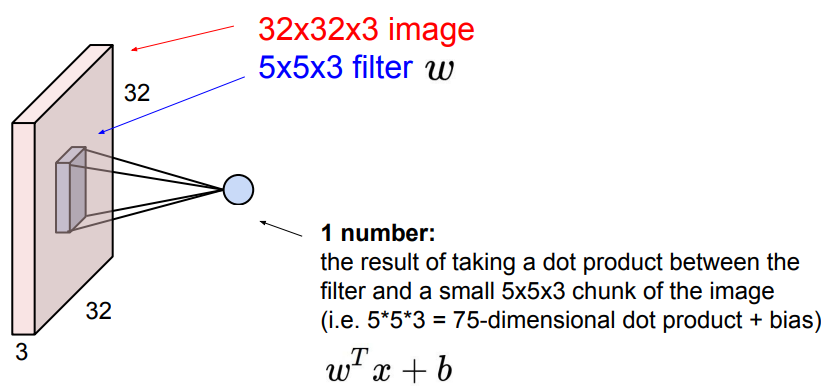
\includegraphics[scale=0.3]{Images/CNNs/kernel1.png}
\end{center}
It is almost always the case that $D = 3$, so we will keep it to $3K^2 + 1$. A possible hyperparameter that needs to be set is the value of $K$, determining the \textbf{width} of the kernel. Another hyperparameter is the \textbf{stride} of the kernel, which determines how many pixels you want the filter to move. The filter will start on the top left of the image and stride (at a certain rate) to the right and down until it reaches the bottom right. Once finished, we should have a transformed image, which we can invoke our activation function $\boldsymbol{\sigma}$ on for each element (pixel) to introduce some nonlinearity. 
\begin{center}
    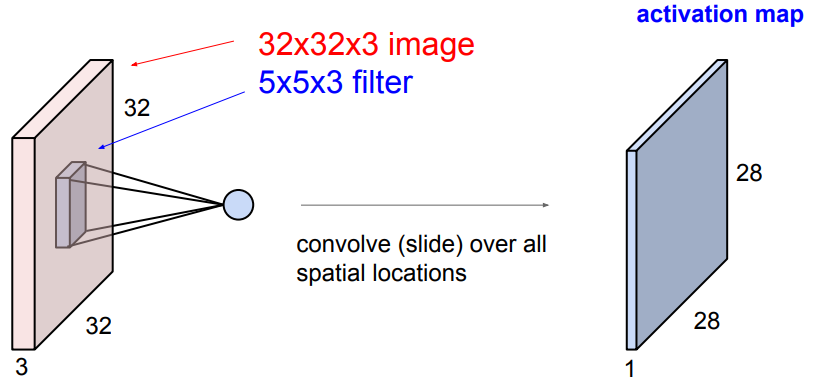
\includegraphics[scale=0.3]{Images/CNNs/kernel2.png}
\end{center}
If one filter $\mathcal{K}$ gives us one output image, then a collection of filters $\mathcal{K}_1, \ldots, \mathcal{K}_l$ (almost always assumed to be of the same size) will give us a collection of $l$ images, or also known as one image of depth $l$. 
\begin{center}
    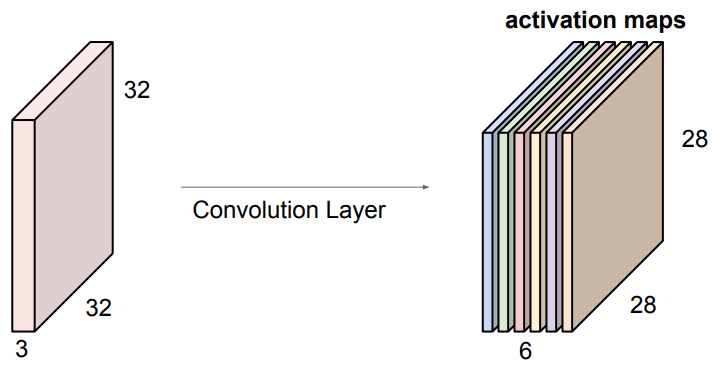
\includegraphics[scale=0.3]{Images/CNNs/kernel3.png}
\end{center}
These convolutions help extract some sort of information, and our choice of convolutions (i.e. the $3K^2$ numbers) will extract different information. Therefore, this is called a \textbf{convolution layer}. As we have more and more convolution layers, we are able to extract from low-level, to mid-level, to high-level features in an image that we can ultimately train on. Ultimately, we would like to stack these layers together enough so that we can have our features, and then we run a few layers of MLP to get our prediction. 


In a way, this is really just a giant sparse matrix multiplication since we can stretch the image out, and each convolution on a pixel is just a linear combination of the pixels around it (plus the ones around it in other channels). In a vanilla MLP, you would optimize all the parameters possible of a linear map over the input images, but a convolutional one takes a very small subset of parameters to optimize, setting everything else to $0$. The weights are furthermore shared/reused across different rows called \textbf{weight sharing}, allowing the model to learn shared representations. There are three reasons that we do this: 
\begin{enumerate}
    \item If the dimensions of the input image was $D_1$ and that of the output image was $D_2$, then we would have to optimize a matrix with $D_1 \times D_2$ parameters. Note that the smallest images in today's standards are $3 \times 256 \times 256 \approx 200,000$ pixels, and so $D_1 \times D_2 \approx 4 \cdot 10^{10}$, which is too many even for one layer. 
    \item There is an MLP way of doing computer vision, and we have performed MLP on very small grayscale images like the MNIST with decent results. Though MLP is more generalized, CNNs have comparable performance at a fraction of the computational cost. 
    \item The images are spatially ordered data. That is, the order in which the pixels are arranged to form the matrix provides a great help in features extraction, so this sense of locality in convolutions help. 
\end{enumerate}


\subsection{Pooling Layers}

Eventually, we would like to use convolutional layers to extract perhaps a few hundred or thousand features that we can then run a MLP on for the last few layers, followed by whatever final activation function needed for prediction. The problem is the high-dimensionality of our inputs. Recall that even the smallest images are $3 \times 256 \times 256 \approx 200,000$ pixels. Even after multiple convolutional layers, the dimensions may not decrease as fast as we want, so we introduce \textbf{pooling layers}, which are efficient layers that decrease the dimension of its inputs in a controlled way, called \textbf{downsampling}. 
\begin{center}
    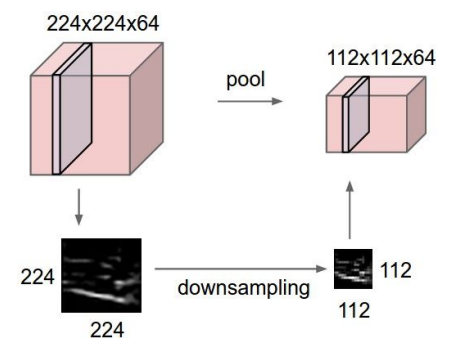
\includegraphics[scale=0.3]{Images/CNNs/max_pool1.png}
\end{center}
We can think of this as decreasing the resolution of the image, and the most common way is through \textbf{max pooling}. You basically have a $P \times P$ square window with some stride, and for each stride, we take the largest value in the window. 
\begin{center}
    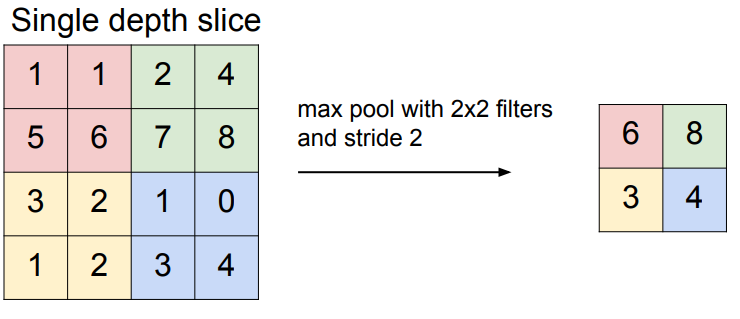
\includegraphics[scale=0.3]{Images/CNNs/max_pool2.png}
\end{center}

\subsection{Backpropagation}


\subsection{Total Architecture with PyTorch}

We have a bunch of convolutional layers with RELU, along with some pooling layers in between. Once we've done enough pooling, we just stretch the resulting image out and run a MLP on the rest with a softmax link function. 
\begin{center}
    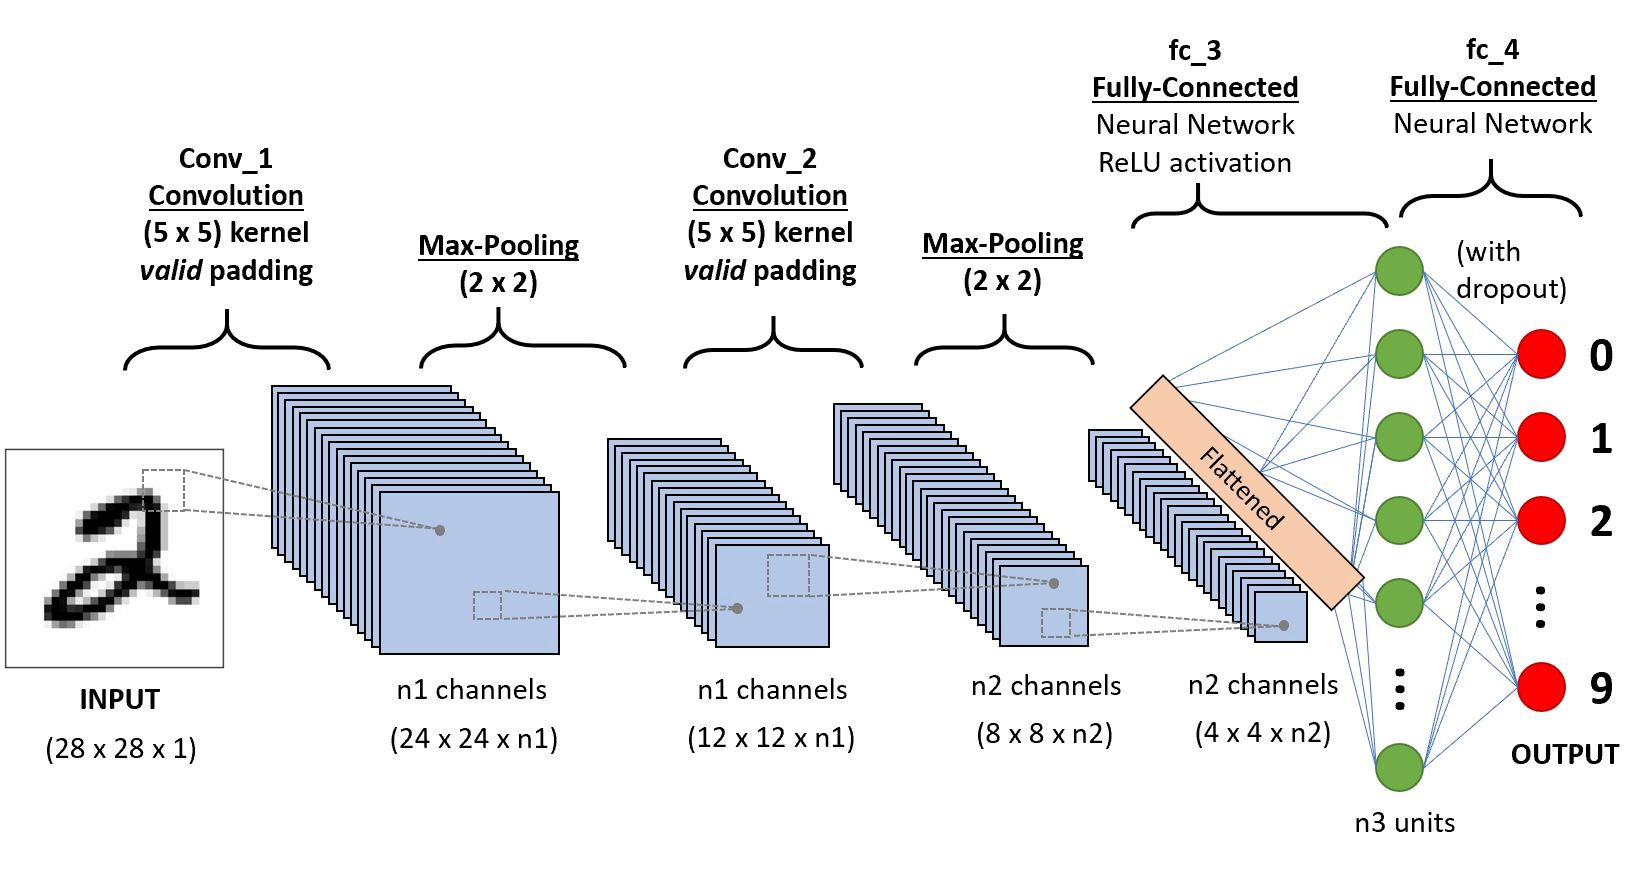
\includegraphics[scale=0.25]{Images/CNNs/CNN_architecture.jpeg}
\end{center}

We can implement it directly in PyTorch by calling $\texttt{nn.Conv2d}()$, where the parameters are number of input channels, number of output channels, and size of kernel (along with optional stride, padding, bias parameters), and $\texttt{nn.MaxPool2d()}$, which take in the kernel size and stride. The rest of the code is completely the same. 
\begin{cverbatim}
class NeuralNetwork(nn.Module):
    # Convolutional Neural Network 

    def __init__(self):
        super().__init__()
        self.conv1 = nn.Conv2d(3, 6, 5)
        self.pool = nn.MaxPool2d(2, 2)
        self.conv2 = nn.Conv2d(6, 16, 5)
        self.fc1 = nn.Linear(16 * 5 * 5, 120)
        self.fc2 = nn.Linear(120, 84)
        self.fc3 = nn.Linear(84, 10)


    def forward(self, x):
        x = self.pool(F.relu(self.conv1(x)))
        x = self.pool(F.relu(self.conv2(x)))
        x = torch.flatten(x, 1) # flatten all dimensions except batch
        x = F.relu(self.fc1(x))
        x = F.relu(self.fc2(x))
        x = self.fc3(x)
        return x
\end{cverbatim}


\subsection{Object Detection} 

So far, we have talked about classification, but this is fundamentally a different problem than object detection. Many aspects will be shared between the two problems. Essentially in detection algorithms, we try to draw a bounding box around the object of interest to locate it within the image. There could be many bounding boxes representing different objects of interest, and what makes this so challenging is that we don't know how many beforehand. Because of these bounding boxes, we must use models that predict also the number and the dimensions of these boxes, use datasets that provide these bounding boxes in addition to labels (e.g. COCO, VOC), and finally we must construct loss functions that take into consideration these boxes. 

Therefore, the major reason why you cannot proceed with this problem by building a standard CNN followed by a fully connected layer is that the length of the output layer is variable. A naive approach to solve this problem would be to take different regions of interest from an image and use a CNN to classify the presence of the object within that region. That is, we do the following steps. 
\begin{enumerate}
    \item We have an input image $\mathbf{x}$, and we want to define a set of subimages $\mathcal{R}$. Each element of $\mathcal{R}$ is essentially a box that segments out a portion of the image $\mathbf{x}$, and we can parameterize this box with 4 numbers. Two of the most popular ones is to take the center of the box plus the width and height $(c_x, c_y, w, h)$ or to take the top-left and bottom-right corners $(x_{min}, y_{min}, x_{max}, y_{max})$. Essentially, we have a giant set of vectors in $\mathbb{R}^4$, and each element is called a \textbf{region of interest}. 
    \item We now take each ROI and input this to our trusty CNN and do the classificaiton task that we have studied up until now. This should tell us whether there is our object of interest in the image or not, and if it passes a certain threshold, we can have it infer that this ROI contains the object. If multiple ROIs pass the threshold, then we can pick the ROI for which the CNN outputs the highest probability of the object existing in.  
\end{enumerate}

This workflow essentially just extracts the regions of interest and does vanilla classification on them. This is an intuitive extension of what we know, but there are a few problems with this approach: 
\begin{enumerate}
    \item A small problem is that the ROIs in $\mathcal{R}$ may not be the same size, while our CNN feature extractor requires its inputs to be fixed. However, this isn't too bad since we can just resize the ROIs for preprocessing. We could also just have $\mathcal{R}$ contain all images of the same size, but this will really hamper the robustness of the model. Objects can be of different size, and so intuitively, we must have different sized ROIs. 
    \item There is the bigger question of how we actually construct $\mathcal{R}$. We have a tradeoff. If $\mathcal{R}$ is too small, it may not capture the structure of the objects of interest. If it is too large, then we may have a combinatoral explosion of ROIs to look for. For example, if we simply have a sliding window with a stride of $1$ that adds each image into $\mathcal{R}$, for an $N \times N$ image we would have $O(N^2)$ ROIs, and this is only for one resolution! This may have been feasible if we were working with linear models, but in the deep learning regime this is not. This second problem is what we will focus on when explaining R-CNNs. i
    \begin{center}
        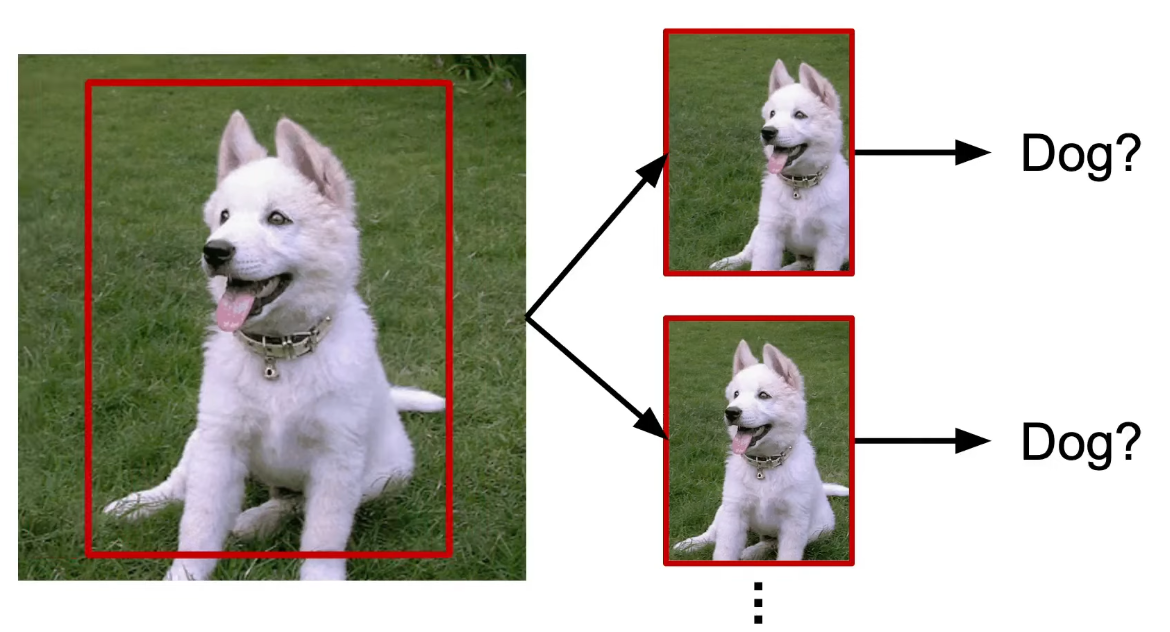
\includegraphics[scale=0.3]{Images/sliding_window.png}
    \end{center}
\end{enumerate}

\subsubsection{Region-Based CNN}

The region-based CNN first bounds $|\mathcal{R}| \leq 2000$ and uses classical image processing techinques to reduce the number of ROIs to less than $2000$. 
\begin{enumerate} 
    \item We start off by using the \textbf{selective search algorithm}. It over-segments the image into seed regions, with each region generating a bounding box. This leads to a ton of regions to look for, and to reduce $|\mathcal{R}|$, we use a greedy algorithm to recursively combine similar regions into larger ones. The segmentation algorithm is the basis of the region proposals, since it matches similar pixels together for a good intialization, giving us the best balance between computational feasibility and quality of proposals. It is specifically designed to have high recall, but low precision, which means that it returns many false positive regions, but are quite certain that they contain the objects of interest.  
    \begin{center} 
        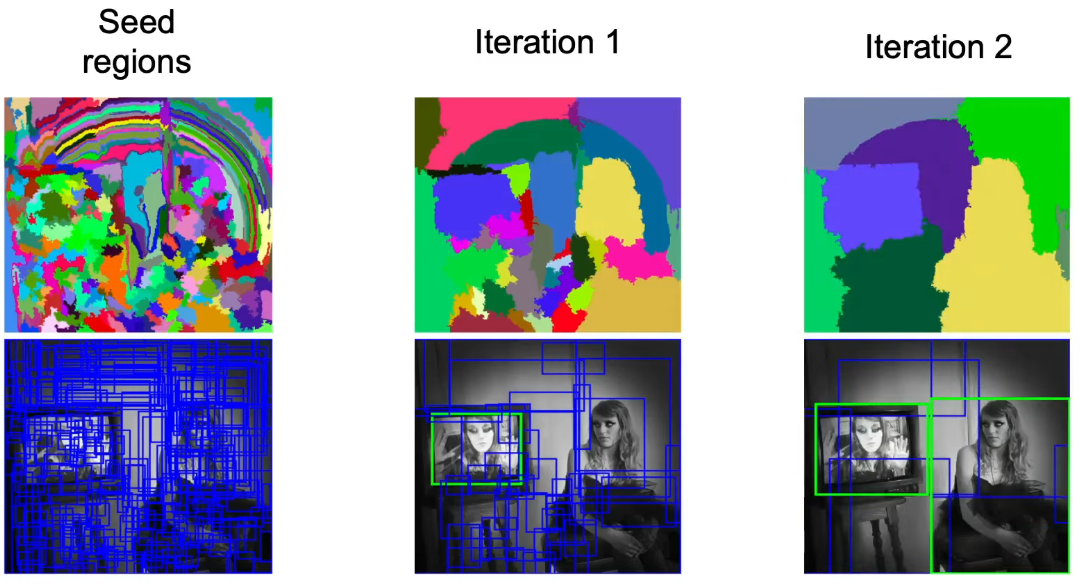
\includegraphics[scale=0.3]{Images/selective_search.png} 
    \end{center}
    \item This usually leads to about 2000 ROIs, and for each ROI, we warp them into a square and feed them into a CNN, which produces a $4096$-dimensional feature vector as output. 
    \item The CNN acts as a feature extractor and the output dense layer consists of the feature extracted from the image. This $4096$-vector is fed into a support vector machine to classify the presence of the object within that candidate region proposal. 
\begin{center}
    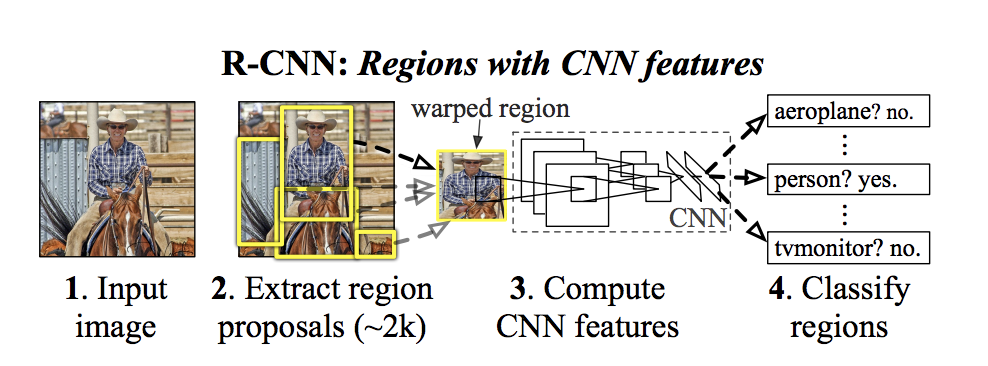
\includegraphics[scale=0.4]{Images/rcnn_diagram.png}
\end{center}

    \item In addition to predicting the presence of an object within the region proposals, the algorithm also predicts 4 values which are offset values to increase the precision of the bounding box. For example, given a region proposal, the algorithm would have predicted the presence of a person but the face of that person within that region proposal could have been cut in half. Therefore, these offset values can help in adjusting the bbox.  
\begin{center}
    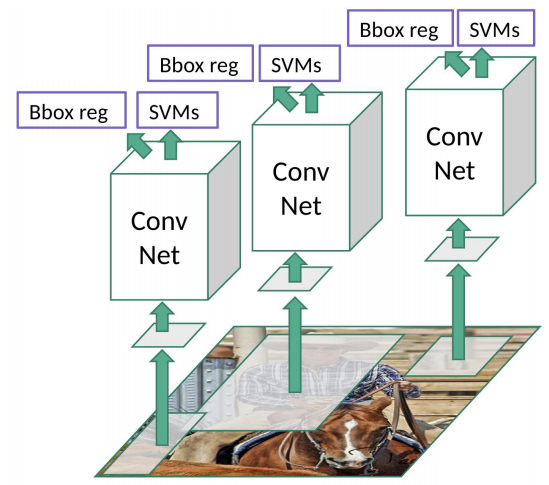
\includegraphics[scale=0.5]{Images/rcnn_diagram2.png} 
\end{center}
\end{enumerate}



However, there are still several problems: 
\begin{enumerate}
    \item While we have improved the computational cost by a lot, we still have to run the CNN feature extractor on \textit{each} of the $2000$ region proposals, which is still too slow for real time inference (takes about 47 seconds), and it takes too long to train. 
    \item When we reshape each region proposal into a square, it may warp the image, causing it to lose its original features. 
    \item The selective search algorithm is not a learning algorithm, so it may generate bad candidate region proposals for various types of images.  
    \item Finally, the R-CNN model is not trained on an end-to-end fashion (the SVM) is trained separately, so this may reduce potential performance. 
\end{enumerate} 

\begin{definition}[IOU]
To provide a measure of how good these boxes are, we use the \textbf{intersection over union (IOU)} metric. If $B$ is the true bounding box and $\Tilde{B}$ our estimate of it, then we have 
\[\mathrm{IoU} = \frac{\mu(B \cap \Tilde{B})}{\mu(B \cup \Tilde{B})}\]
The closer it is to $1$, the better, and a ``good" match is defined to be $0.7$ or above.  
\end{definition} 


\subsubsection{Fast RCNN}

Fast RCNN is basically just RCNN but with a few tweaks to make it fast. The computational bottleneck came from having to run a CNN on each of the 2000 region proposals, but now, to speed things up, we have a CNN extract features from the whole image first. We describe the steps below. 
\begin{enumerate} 
    \item We take the image $\mathbf{x} \in \mathbb{R}^{n \times m}$ and use the CNN $f$ to extract features from it, resulting in say $\boldsymbol{\phi} \in \mathcal{F}$.
    \item At the same time, we run the selective search algorithm on $\mathbf{x}$ to get our region proposals $\mathcal{R}$. 
    \item For each region of interest $\mathbf{r} \in \mathcal{R}$, we project the resulting regions coordinate into the feature map $\mathcal{F}$. Note that we are not running inference here, just projecting, so this is computationally cheap and allows us to reduce the computational cost of extracting features by an order of $2000$. Specifically, if there is a convolution on a ROI with stride 1 and the proper padding, the regions will have the same coordinates. Meanwhile, if we have a max pooling layer, then each coordinate $(x, y)$ will get mapped to $(\lceil x/2 \rceil, \lceil y/2 \rceil)$. 
    \item After this projection, for every $\mathbf{r} \in \mathcal{R}$, we have its projections $p(\mathbf{r}) \in \mathcal{F}$. However, this projection is not the same le,gth for all region proposals, so we have a \textbf{RoI pooling layer} which takes each projected region, divides it into a fixed number of bins (independent of the input shape), and does max pooling over each bin to generate a fixed feature vector for each region proposal.
    \begin{center}
        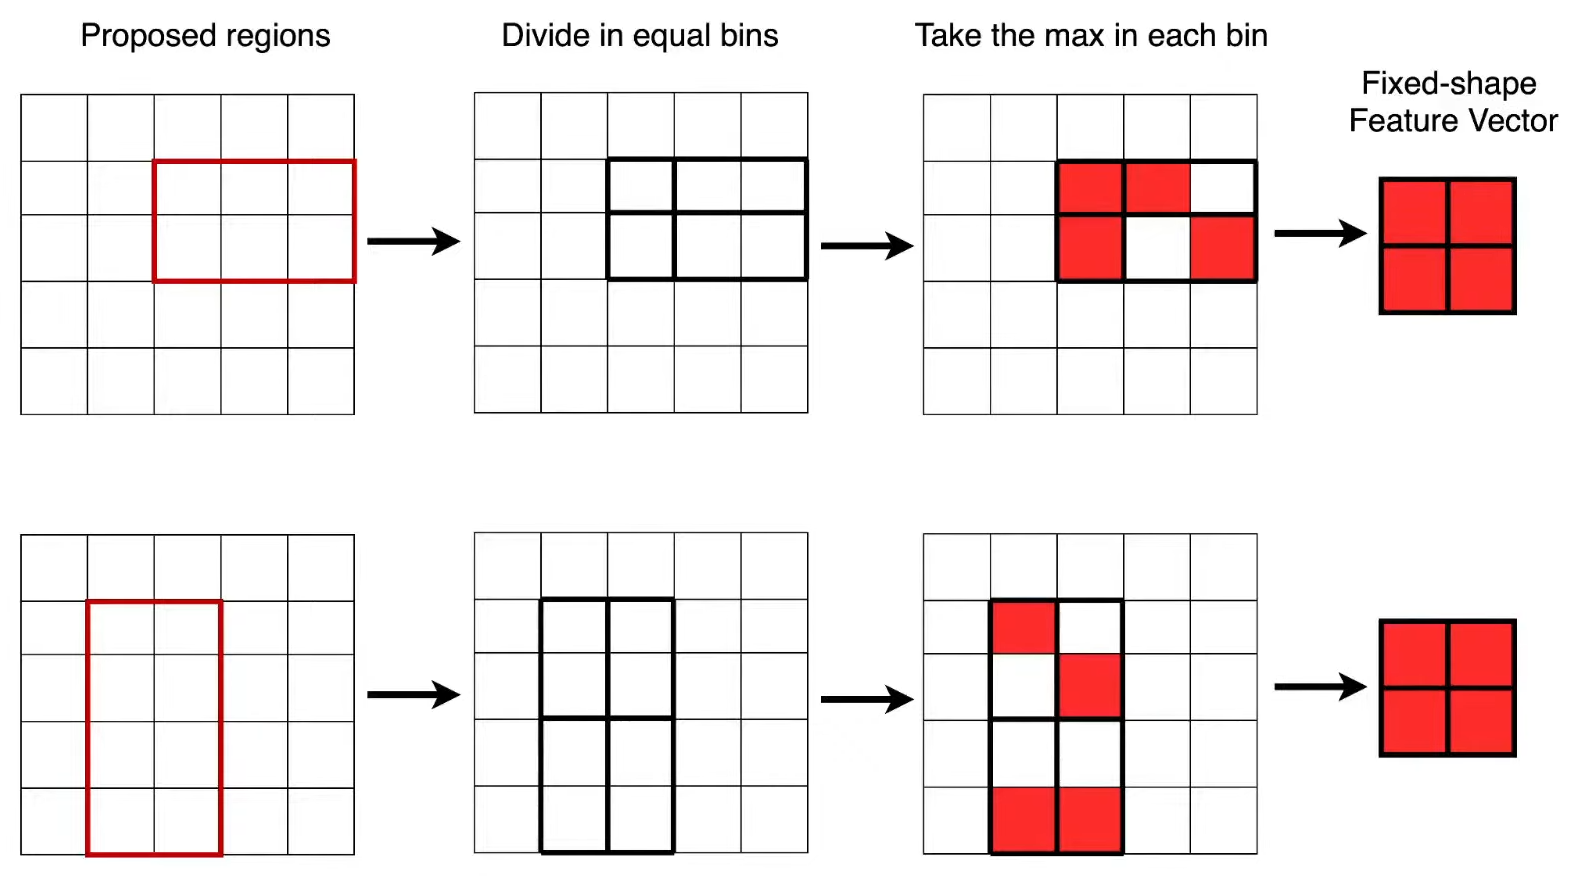
\includegraphics[scale=0.3]{Images/roi_pooling.png} 
    \end{center}
    \item Then we take these fixed size feature vectors and feed them through a fully connected neural network to get a feature vector where we can do softmax classification on, along with regression of the bboxes dimensions. 
\end{enumerate}

\begin{center}
    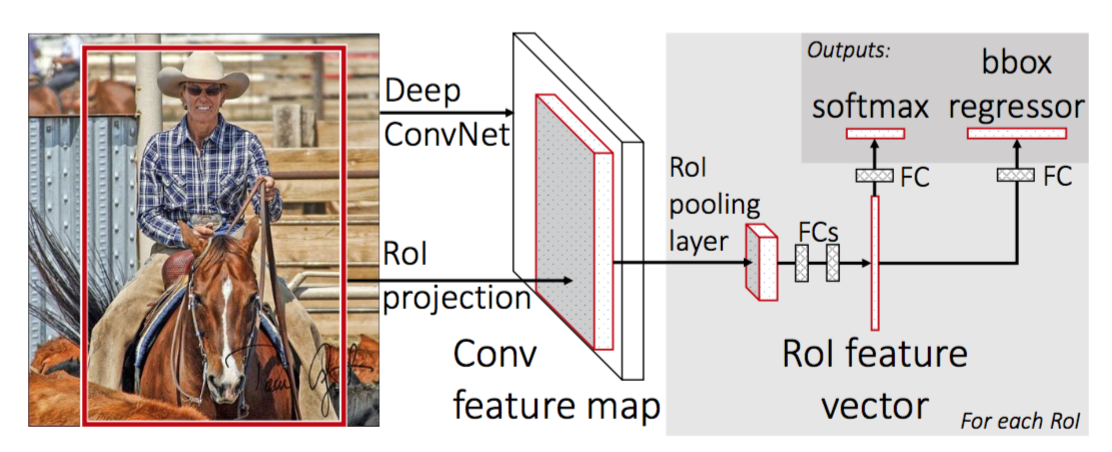
\includegraphics[scale=0.3]{Images/fast_rcnn.png}
\end{center}

Regarding the problems, this first improves the computational cost compared to R-CNN. By utilizing the IOU pooling layers, we have resized the images after the CNN feature extractor rather than distorting the original input itself. Moreover, we have replaced the SVM classifiers with neural nets. However, we still have the problem that the region proposal algorithm is an external algorithm that's not learned, and this selective search method still turns out to be quite slow for real-time inference.  

\subsubsection{Faster RCNN}

Therefore, Ren et al, came up with an object detection algorithm that eliminates the selective search algorithm and lets the network learn the region proposals. The Faster RCNN model essentially repalces the region proposal algorithm with a significantly faster neural network that can learn to propose better regions for the task at hand. 
\begin{center}
    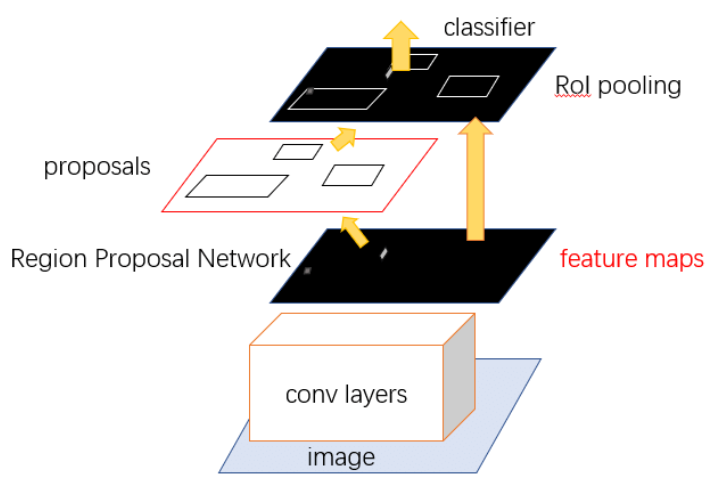
\includegraphics[scale=0.4]{Images/faster_rcnn_diagram.png}
\end{center}

Let's walk through the steps of this algorithm: 
\begin{enumerate}
    \item We take the image $\mathbf{x}$ and run it through a backbone convolutional network (usually the first few layers of ResNet or VGG), generating a feature map $\phi \in \mathbb{R}^{K \times K}$. There are $K^2$ ``points" or ``pixels" in this feature representation of $\mathbf{x}$, and \textbf{anchor points} are generated on $\phi$ . If they are projected back into the original image, we would have $K^2$ equally spaced points over $\mathbf{x}$. 
        \begin{center}
            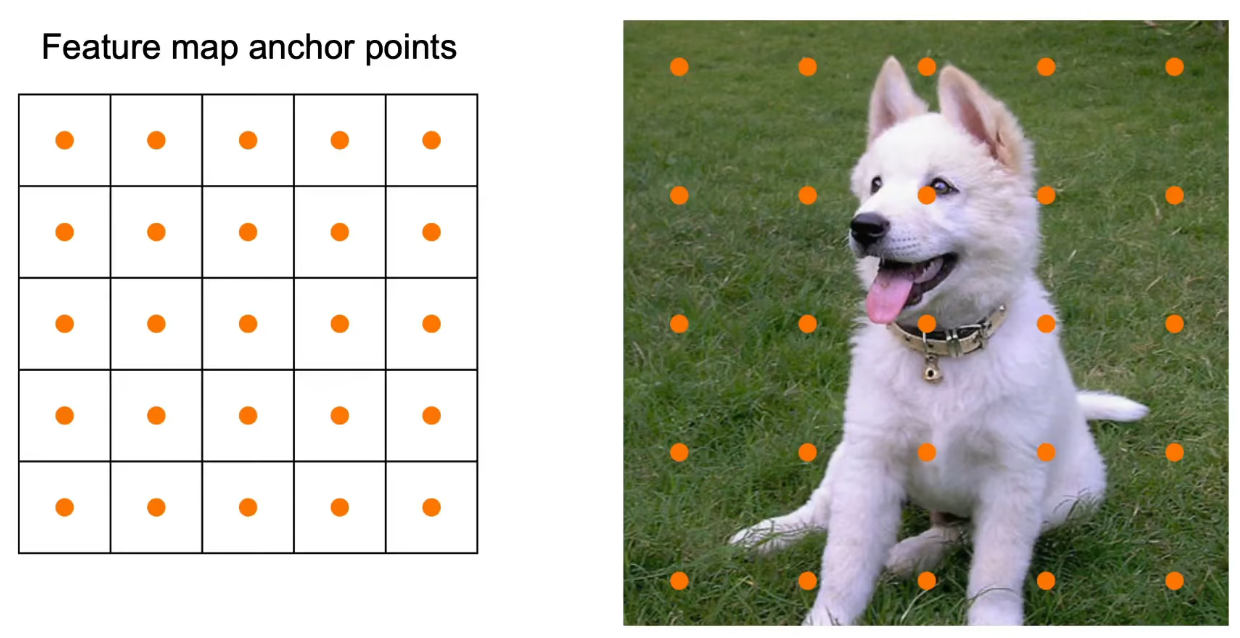
\includegraphics[scale=0.2]{Images/anchor_points.png}
        \end{center}
    \item For each anchor point, we have $k$ predefined boxes of different sizes and aspect ratios that are used to generate region proposals that may or may not contain objects of interest. For example, we can have $k = 4$ in the picture below. 
    \begin{center}
        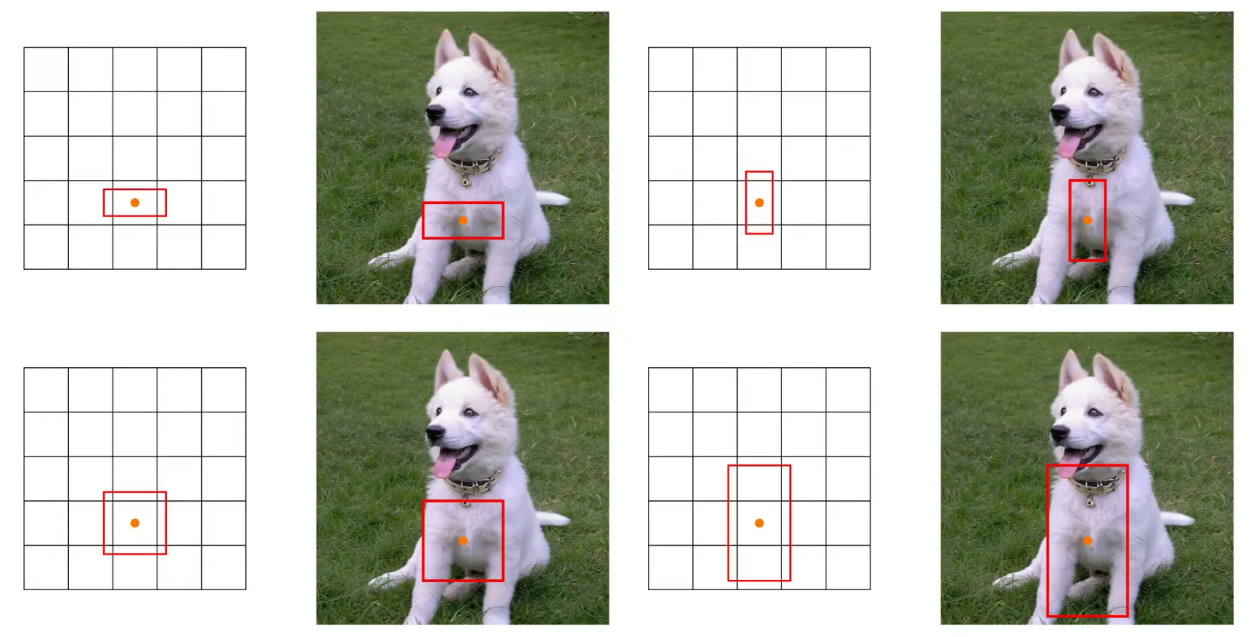
\includegraphics[scale=0.2]{Images/anchor_boxes.png}
    \end{center}
    \item At this point, we have a total of $k K^2$ total anchor boxes on the feature space. We project all this back to the original image space, and we look for the samples that have a good IoU (calculated in the feature space with the projected ground truth boxes!) with the ground truth bbox. We generate (usually an equal amount) of positive and negative samples from the $k K^2$ total boxes. 
    \begin{center}
        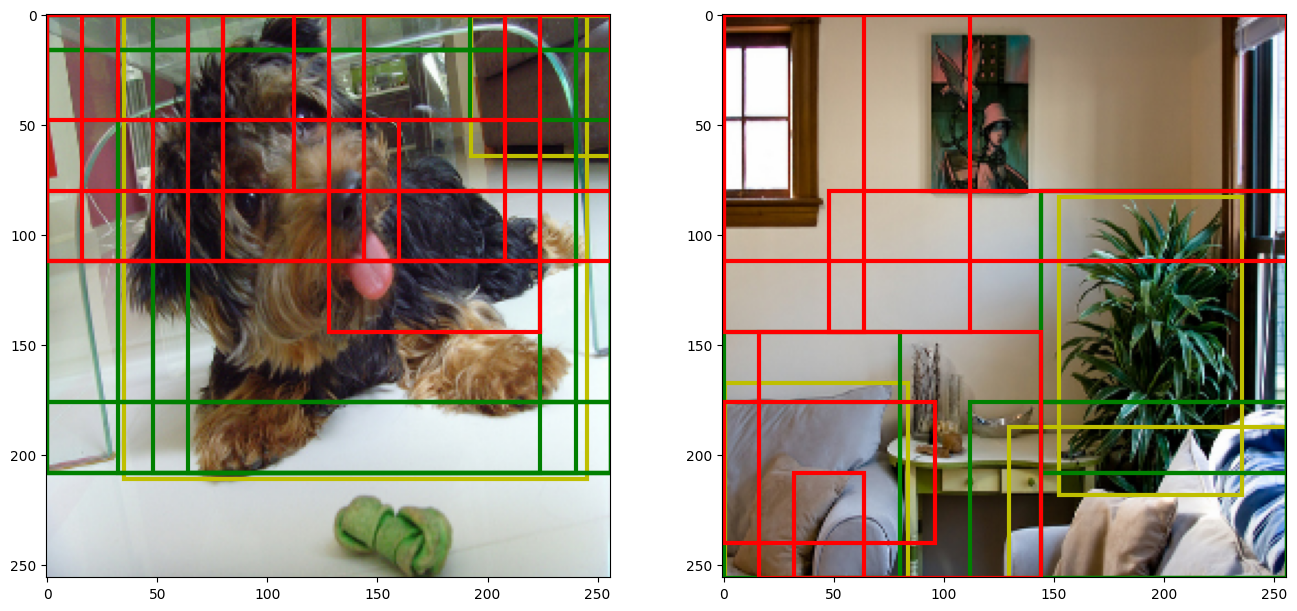
\includegraphics[scale=0.2]{Images/gt_sampling.png}
    \end{center}
    
    \item For each of the $k K^2$ boxes, we want to classify each as an object or background, along with predicting their offsets from the corresponding gt bboxes. To do this, we use $1 \times 1$ convolutional layers. We take the feature map, which is of shape $(C, K, K) = (2048, 8, 8)$ and use the kernel to give us an output of size $(k, K, K)$. This output basically labels each of the $k K^2$ anchor boxes with some scalar that represents whether we think it is an object or background. We take a second $1 \times 1$ kernel and have it output $(4k, K, K)$ representing the offsets of the bounding boxes. This is called the regression head, and we need $4k$ since there are 4 degrees of freedom in adjusting each bounding box. 
    
    \item Now we have the scores and offsets of all the anchor boxes. But during training we only select the positive and negative anchor boxes to compute classification loss, and only positive boxes to compute the L2 regression loss. 

    \item In this second stage, we receive region proposals and predict the category of the object in the proposals. These region proposals (due to the anchor boxes being different sizes) are not the same size, so we use RoI pooling just like in Fast RCNN. After this, it's the same: we pass them through a fully connected MLP with some softmax and regressor link. 

    \item During inference, we pass the image through the backbone network to generate anchor boxes. Then, we select only the top ~300 boxes that get a high classification score and qualify them for the next stage. We then predict the final categories and offsets, performing an extra post-processing step called non-max surpression to remove duplicate bounding boxes. 
\end{enumerate}

Note that since we are using convolutions, this makes the object detection algorithm translationally invariant, and rotational invariance can be achieved through data augmentation. 

\subsubsection{Measuring Performance} 

Recall that if we are just predicting the presence of 1 class, then we can talk about the recall or precision. A better way is to look at the mean precision, which is found by taking the integral of the precision recall curve. Other metrics include the $F_1$ score. 
\[\text{Precision} = \frac{TP}{TP + FP}, \; \text{Recall} = \frac{TP}{TP + FN}, \; F_1 = 2 \frac{\text{Precision} \cdot \text{Recall}}{\text{Precision} + \text{Recall}}\]
For multiple classes, we can use the \textbf{mean average precision}, which is basically the average precision for multiple classes.

\section{Linear Factor Models}

Throughout this course, neural networks have been used as feature extractors of some high-dimensional input. We have trained the network to pick good features, which live in some vector space that is directly relevant to what our prediction should be. Often, this vector space is not interpretable and can be seen as a \textbf{latent space} of \textbf{hidden/latent variables}. In unsupervised learning, constructing a good latent representation of our data can be extremely useful. 

Say that we want to do density estimation for the probability distribution of the covariates $\mathbf{x}$. We can try to model it directly, but this may be infeasible. Rather, what we do is ``add" a latent distribution $\mathbf{z}$, creating the joint distribution $(\mathbf{x}, \mathbf{h})$. This may look more complicated, but what we hope to find is that 
\[p(\mathbf{x}) = \mathbb{E}_{\mathbf{h}} [ p(\mathbf{x} \mid \mathbf{h})]\]
That is, we hope that we can model the latent $\mathbf{h}$ in a simple form, and we can therefore decompose $p(\mathbf{x})$ into some random variable dependent on $\mathbf{h}$. Therefore, we've modeled $p(\mathbf{x} \mid \mathbf{h})$ by assumption, and with this we can compute $p(\mathbf{x}, \mathbf{h}) = p( \mathbf{x} \mid \mathbf{h}) \, p( \mathbf{h})$, allowing us to compute 
\[p( \mathbf{x}) = \int p(\mathbf{x} \mid \mathbf{h}) \, p(\mathbf{h}) \, d\mathbf{h}\]
Like we do with everything else in math, we take a look at the simplest example: linear functions. 

In \text{linear factor models}, we start with the unknown covariate distribution $\mathbf{x} \in \mathbb{R}^d$, and we create a latent variable $\mathbf{h} \in \mathbb{R}^k$ ($k$ is to be chosen). We first assume that 
\[\mathbf{h} \sim p(\mathbf{h})\] 
comes from some predefined distribution, with the only constraint being that it is factorable (i.e. is the product of its marginal distributions: $p(\mathbf{h}) = \prod_i p(h_i)$) so that it is easy to sample from. Occasionally, the stronger assumption of the $h_i$'s being iid is made. Then, we assume that 
\[\mathbf{x} = \mathbf{W} \mathbf{h} + \mathbf{b} + \epsilon\] 
where the noise $\epsilon$ is typically Gaussian and diagonal (but not necessarily the same component-wise variances). Finally, we can use techniques like MLE to estimate $\mathbf{W}, \mathbf{b}$, and the parameters of $\epsilon$.  

The entire reason we want to do this is that we are hoping that $\mathbf{h} \in \mathbb{R}^k$ and $\mathbf{x} \in \mathbb{R}^d$, and $d >> k$. Therefore, $\mathbf{W}$ is a $d \times k$ matrix, and the latent variables $\mathbf{h}$ give a more compact (parsimonious)  explanation of dependencies between the components of the observations $\mathbf{x}$. The following are all special cases of linear factor models: 
\begin{enumerate}
    \item Probabilistic PCA
    \item Factor Analysis
    \item Independent Component Analysis (ICA)
\end{enumerate}

\subsection{Factor Analysis and Probabilistic PCA}

\begin{example}[Factor Analysis] 
Factor analysis is a specific case of a linear factor model where 
\[\mathbf{x} = W \mathbf{h} + b + \epsilon, \text{ where } \mathbf{h} \sim N(\mathbf{0}, \mathbf{I}), \; \epsilon \sim N(0, \sigma^2)\] 
It should be clear to us that $\mathbf{x}$ should be Gaussian and that $\mathbb{E}[\mathbf{x}] = \mathbf{b}$, with 
\begin{align*} 
    \mathrm{Var}[\mathbf{x}] & = \mathbb{E}[ (\mathbf{x} - \mathbf{b})( \mathbf{x} - \mathbf{b})^T ] \\
                             & = \mathbb{E}[ (W \mathbf{h} + \epsilon) (\mathbf{h}^T W^T + \epsilon^T)] \\
                             & = \mathbb{E}[W h h^T W^T] + \mathbb{E}[ \epsilon \epsilon^T] \\
                             & = W \mathbb{E}[ h h^T] W^T + \mathbb{E}[ \epsilon \epsilon^T] \\
                             & = W W^T + \mathrm{diag}(\sigma_1^2, \ldots, \sigma_d^2) 
\end{align*} 
The $\mathbf{W}, \mathbf{b}$, and $\boldsymbol{\sigma}$ can be estimated using MLE methods. Unfortunately, no closed form  exists, so iterative methods are commonly applied. 
\end{example} 

Note that in here, we do not assume that the variances of the $h_i$'s are the same, though they are independent. This means that the subspace generated by the MLE estimate of $\mathbf{W}$ will not necessarily correspond to the principal subspace of the data. But we can make this happen with one more assumption. Before we get into probabilistic PCA, let's review regular PCA. 

\begin{example}[PCA] 
    
\end{example} 

\begin{example}[Probabilistic PCA] 
In PPCA, we assume everything we did for factor analysis, but now also that $\sigma_1 = \ldots = \sigma_k = \sigma$. In this case, 
\[\mathbf{x} \sim N(\mathbf{b}, \mathbf{W}\mathbf{W}^T + \sigma^2 \mathbf{I})\]
and the MLEs for $\mathbf{W}, \mathbf{b}, \sigma$ have a closed form, and model parameter estimation can be performed iteratively and efficiently. We define. It is pretty clear that 
\[\hat{\mathbf{b}}_{MLE} = \frac{1}{N} \sum_{i=1}^N \mathbf{x}^{(i)}\]
and setting 
\[\widehat{\mathrm{Var}}_{MLE}(\mathbf{x}) = S = \frac{1}{N} \sum_{i=1}^N (\mathbf{x}^{(i)} - \mathbf{b}) (\mathbf{x}^{(i)} - \mathbf{b})^T\]
which is the biased, but MLE estimator of the variance, let us derive the MLE of $\mathbf{W}$. Say that $\mathbf{W}^\ast$ is an MLE, then, for any unitary $\mathbf{U} \in \mathbb{R}^{k \times k}$, we have 
\[\mathbf{W}^\ast \mathbf{W}^{\ast T} = (\mathbf{W}^\ast \mathbf{U}) (\mathbf{W}^\ast \mathbf{U})^T \]
which means that the MLE is not unique. We can find the MLE estimate of $\sigma$ first by taking a look at $C = \mathrm{Var}[\mathbf{x}] = \mathbf{W} \mathbf{W}^T + \sigma^2 \mathbf{I}$. It is the sum of positive semidefinite patrices that are also symmetric, so by the spectral theorem it is diagonalizable and has full rank $d$. But $\mathbf{W} \mathbf{W}^T$ is rank $k$, so $d - k$ of the eigenvalues of $\mathbf{W} \mathbf{W}^T$ is $0$, indicating that the same $d-k$ smallest eigenvalues of $C$ is $\sigma^2$. Therefore, we can take the smallest $d-k$ eigenvalues of our MLE estimator of $C$, which is $S$, and average them to get our MLE for $\sigma$. 
\[\hat{\sigma}^2_{MLE} = \frac{1}{d-k} \sum_{j=k+1}^d \lambda_j\]
We can approximate $\mathbf{W} \mathbf{W}^T = C - \sigma^2 \mathbf{I} \approx S - \hat{\sigma}^2_{MLE} \mathbf{I}$, and by further taking the eigendecomposition $C = U \Sigma U^T \implies \mathbf{W} \mathbf{W}^T = U (\Sigma - \sigma^2 \mathbf{I}) U^T$ and cutting off the last $d-k$ smallest eigenvalues and their corresponding eigenvectors, we can get 
\[\mathbf{W}_{ML} = \mathbf{U}_q (\Lambda_d - \hat{\sigma}_{MLE}^2 \mathbf{I}_d )^{1/2} R\] 
where the $R$ just accounts for any unitary matrix. 
\end{example}

Now as $\sigma \rightarrow 0$, the density model defined by PPCA becomes very sharp around these $d$ dimensions spanned by the columns of $\mathbf{W}$. At $0$, our MLE of $W$ is simplified and we have 
\[\mathbf{x} = \mathbf{W}_{MLE} \mathbf{h} + \mathbf{b}_{MLE} + \epsilon = \mathbf{U}_q \boldsymbol{\Lambda}_q^{1/2} \mathbf{h} + \mathbf{b}_{MLE} \]
which essentially reduces to regular PCA. That is, the conditional expected value of $\mathbf{h}$ given $\mathbf{x}$ becomes an orthogonal projection of $\mathbf{x} - \mathbf{b}$ onto the subspace spanned by the columns of $\mathbf{W}$.  


\subsection{Independent Component Analysis} 

Another special case of linear factor model is ICA. In our setting, let us just assume that $\mathbf{b} = \mathbf{0}$ and $\epsilon = 0$. That is, we have the simple model 
\[\mathbf{x} = \mathbf{W} \mathbf{h}\] 
In here, $\mathbf{x} \in \mathbb{R}^d$ is a mixture vector and $\mathbf{W} \in \mathbb{R}^{d \times d}$ is a \textbf{mixing matrix}. Note that the hidden $\mathbf{h}$ has the same dimensions as $\mathbf{x}$, but this can be generalized to rectangular matrices. Both $\mathbf{W}$ and $\mathbf{h}$ are unknown, and we need to recover them given $\mathbf{x}$. In \textbf{linear ICA}, we have two strong assumptions: 
\begin{enumerate} 
    \item Each component of $\mathbf{h}$ is independent (not just uncorrelated). This is an easy enough assumption to intuit.  
    \item Independent components of $\mathbf{h}$ must \textit{not} be Gaussian. This is needed for us to be able to ``unmix" the signals. To see why, just suppose $\mathbf{h}$ was Gaussian, and so the vector $\mathbf{R} \mathbf{h}$ is also Gaussian for any invertible $\mathbf{R}$. Therefore, we could find an infinite number of solutions of form 
    \[\mathbf{x} = \mathbf{W} \mathbf{R}^{-1} \mathbf{R} \mathbf{h}\]
    and I have no way to separate them. 
\end{enumerate}

There are further ambiguities with ICA. 
\begin{enumerate}
    \item Estimating the latent components up to a scaling factor. 
        \[\mathbf{x} = (\alpha \mathbf{W}) (\frac{1}{\alpha} \mathbf{h}) \text{ for some } \alpha > 0\]
        We can fix this by forcing $\mathbb{E}[h_i^2] = 1$. However, there is still an ambiguity for the sign of hidden components, but this is insignificant in most applications. 

    \item Estimating the components up to permutation. We have 
        \[\mathbf{x} = \mathbf{W} \mathbf{P}^{-1} \mathbf{P} \mathbf{h}\] 
        for some permutation matrix $\mathbf{P}$. 
\end{enumerate}

Now let's see how linear ICA actually estimates $\mathbf{W}$ and $\mathbf{h}$. Once $\mathbf{W}$ is estimated, the latent components of a given test mixture vector, $\mathbf{x}^\ast$ is computed by $\mathbf{h}^\ast = \mathbf{W}^{-1} \mathbf{x}^\ast$. So now all there's left to do is to estimate $\mathbf{W}$, which we want to estimate so that $\mathbf{W}^{-1} \mathbf{x}$ is far from Gaussian. The reason for this is that given a bunch of independent non-Gaussian $h_i$'s, if we mix them with a matrix that is not $\pm \mathbf{I}$ , then by CLT, a linear combination of random variables will tend to be Gaussian, and so for an arbitrary $\mathbf{W}$ we would expect $\mathbf{x}$ to be Gaussian. Therefore, what we want to do is guess some matrix $\mathbf{A}$, and compute 
\[\mathbf{A} \mathbf{x} = \mathbf{A} \mathbf{W} \mathbf{h}\]
and if we get things right, $\mathbf{A} \approx \mathbf{W}^{-1}$, and the result of $\mathbf{A} \mathbf{x}$ would look pretty non-Gaussian. If it it not the case, then $\mathbf{A W}$ will still be some mixing matrix, and so $\mathbf{A} \mathbf{x}$ would look Gaussian. So now the question reduces to how do we choose this $\mathbf{A}$? There are multiple ways to measure non-Gaussianity: 
\begin{enumerate} 
    \item The absolute or squared kurtosis, which is $0$ for Gaussians. This is a differentiable function w.r.t. $\mathbf{W}$, so we can try maximizing it. This is done for the sample kurtosis, of course.  
    \item Another measure is by maximizing the neg-entropy. 
\end{enumerate}

We can perform this on three mixed signals with additive noise, and ICA does very well, though again some recovered signals are scaled or permuted weirdly. 
\begin{center}
    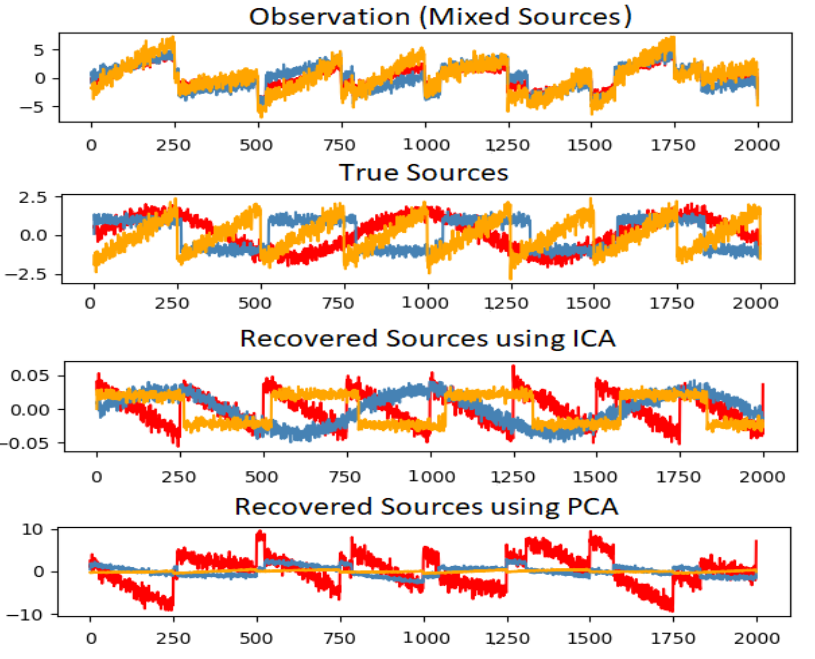
\includegraphics[scale=0.4]{Images/ICA_example.png}
\end{center}

\subsection{Slow Feature Analysis} 

Slow feature analysis also another special case of a linear factor model that uses information from time signals to learn invariant features. It is motivated by a general principle called the \textbf{slowness principle}. The idea is that the important characteristics of scenes change very slowly compared to the individual measurements that make up a description of a scene. For example, in computer vision, individual pixels can change very rapidly. If a zebra moves from left to right across the image, an individual pixel wil rapidly change from black to white. By comparison, the feature indicating whether a zebra is in the image will not change at all, and the feature describing the zebra's position will change slowly. Therefore, we want to regularize our model to learn features that change slowly over time.  

We can apply the slowness principle to any differentiable model trained with gradient descent. That is, we can add the following term to the loss function: 
\[\lambda \sum_i d\big( f(\mathbf{x}^{(t+1)}), f(\mathbf{x}^{(t)}) \big)\]
where $\lambda$ is a hyperparameter determining the strength of the slowness regularization term, $t$ is the time index, $f$ is the feature extractor to be regularized, and $d$ is the distance between $f(\mathbf{x}^{(t)})$ and $f(\mathbf{x}^{(t+1)})$. A common choice for $d$ is the mean squared difference. 

Essentially, given a set of time-varying input signals $\mathbf{x}^{(t)}$, SFA learns a nonlinear function $f$ that transforms $\mathbf{x}$ into slowly-varying output signals $\mathbf{y}$. Obviously, we can't just take some trivial function like $f = 0$, so we have the following constraints 
\begin{align*}
    \mathbb{E}_t [ f(\mathbf{x}^{(t)})_i]  & = 0 \\ 
    \mathbb{E}_t [ f(\mathbf{x}^{(t)})_i^2] & = 1 
\end{align*}
\begin{center} 
    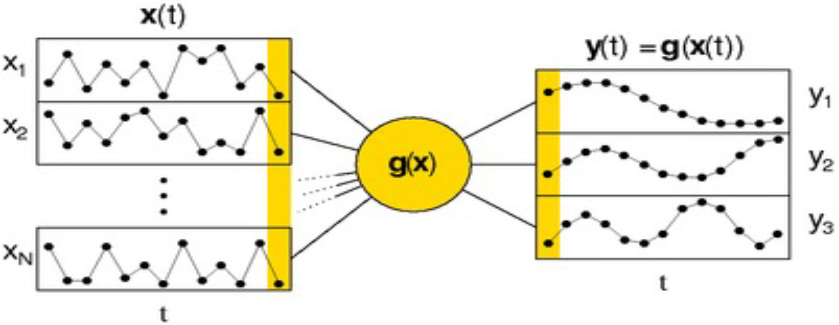
\includegraphics[scale=0.4]{Images/slow_feature.png}
\end{center}
We can restrict the nonlinear $f$ to some subspace of functions, and this becomes a standard optimization problem where we solve 
\[\min_\theta \mathbb{E}_t \big[ \big( f(\mathbf{x}^{(t+1)})_i - f(\mathbf{x}^{(t)})_i \big)^2 \big]\]



\subsection{Sparse Coding}

What we want to do in sparse coding is that for each input $\mathbf{x}^{(t)}$, we want to find a latent representation $\mathbf{h}^{(t)}$ s.t. 1) it is sparse (i.e. has many $0$s) and 2) we can reconstruct the original input $\mathbf{x}^{(t)}$ well. We have basically two things to optimize: the latent representations $\mathbf{h}$ and the decoding mechanism, which we can do with a \textbf{dictionary matrix} $\mathbf{D}$. Therefore, we want to perform the joint optimization
\[\min_{\mathbf{D}} \frac{1}{T} \sum_{t=1}^T \min_{\mathbf{h}^{(t)}} \underbrace{\frac{1}{2} ||\mathbf{x}^{(t)} - \mathbf{D} \mathbf{h}^{(t)}||_2^2}_{\text{reconstruction error}} + \underbrace{\lambda ||\mathbf{h}^{(t)}||_1}_{\text{sparsity penalty}}\]
To break this term down, let's just assume that we have a fixed dictionary $\mathbf{D}$. Then, we just need to minimize with respect to each $\mathbf{h}^{(t)}$. Now we can add the dictionary parameter back again. 

Note that the reconstruction, or decoding, of $\mathbf{x}^\prime = \mathbf{D} \mathbf{h}$ is linear and explicit, but if we want to encode $\mathbf{x} \mapsto \mathbf{h}$, we need to substitute the $\mathbf{x}$ into the term above and minimize it w.r.t. $\mathbf{D}$ and $\mathbf{h}$ to solve it. Therefore, this encoder is an implicit and nonlinear function of $\mathbf{x}$. 

For example, we can reconstruct an image of a seven as a linear combination of a set of images. Note that each of the images of strokes are columns of $\mathbf{W}$ and the coefficients make up the sparse vector $\mathbf{h}$. 
\begin{center}
    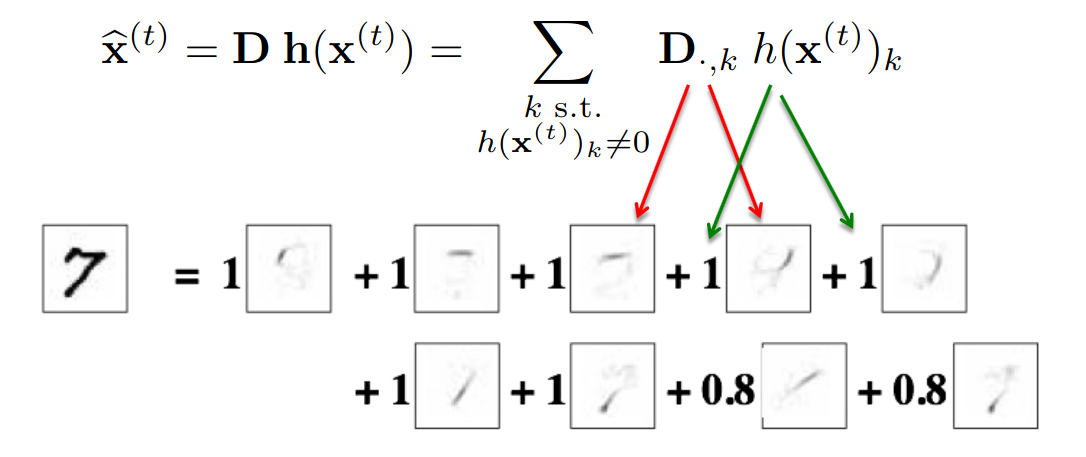
\includegraphics[scale=0.4]{Images/sparse_coding.png}
\end{center}
Let's think about how we can optimize the objective function w.r.t. $\mathbf{h}$, keeping $\mathbf{D}$ constant. We can do stochastic gradient descent, which gives us the steps
\[\nabla_{\mathbf{h}^{(t)}} \mathcal{L}(\mathbf{x}^{(t)}) = \mathbf{D}^T (\mathbf{D} \mathbf{h}^{(t)} - \mathbf{x}^{(t)}) + \lambda \, \mathrm{sign}(\mathbf{h}^{(t)})\]
but this wouldn't achieve sparsity since it overshoots the $0$ all the time. Therefore, we can clip it, or we can use proximal gradient descent/ISTA to take a step, and shrink the parameters according to the L1 norm. 
\begin{align*} 
    \mathbf{h}^{(t)} & = \mathbf{h}^{(t)} - \alpha \mathbf{D}^T (\mathbf{D} \mathbf{h}^{(t)} - \mathbf{x}^{(t)}) \\
    \mathbf{h}^{(t)} & = \mathrm{shrink}(\mathbf{h}^{(t)}, \alpha \lambda)
\end{align*}
    where $\mathrm{shrink}(\mathbf{a}, \mathbf{b}) = [\ldots, \mathrm{sign}(a_i)\, \max(|a_i| - b_i, 0), \ldots]$. This is guaranteed to converge if $1/\alpha$ is bigger than the largest eigenvalue of $\mathbf{D^T} \mathbf{D}$.  

\section{Autoencoders}

Autoencoders are a type of unsupervised learning. We only use the inputs $\mathbf{x}_t$ for learning. We want to automatically extract meaningful features for the data and leverage the availability of unlabeled data. It can be used for visualization and compression. We can also build generative models with autoencoders. 

\begin{definition}[Autoencoder]
    An autoencoder is a feed-forward neural net whose job is to take an input $\mathbf{x}$ and output $\hat{\mathbf{x}}$. It consists of an encoder $E_\phi: \mathcal{X} \rightarrow \mathcal{Z}$ and decoder $D_\theta: \mathcal{Z} \rightarrow \mathcal{X}$, where $\mathcal{X}$ is the input/output space and $\mathcal{Z}$ is the latent feature space. 
\begin{enumerate}
    \item The encoder model transforms $\mathbf{x}$ to a latent feature representation $\mathbf{z}$. It is a feed-foward, buttom-up neural net. 
    \item The decoder model maps $\mathbf{z}$ to a reconstruction $\hat{\mathbf{x}}$. It is generative, top-down. 
\end{enumerate}
I want to train the whole neural network such that the error between $\mathbf{x}$ and $\hat{\mathbf{x}}$ is minimized. We can consider a squared-error, for example. 
\[\mathcal{L}(\mathbf{x}, \hat{\mathbf{x}}) = \frac{1}{2} ||\mathbf{x} - \hat{\mathbf{x}}||_2^2\]
\end{definition}

In the totally linear case, we have PCA. Some input $\mathbf{x} \in \mathcal{X} = \mathbb{R}^d$ is mapped to a smaller-dimensional $\mathcal{Z} = \mathbb{R}^k$. 
\[\mathbf{x} \xlongrightarrow[]{V} \mathbf{z} \xlongrightarrow{U} \hat{\mathbf{x}}\]
and so the ``network" essentially computes $\hat{\mathbf{x}} = U V \mathbf{x}$. Obviously the fact that $k < d$ is essential, since if $k \geq d$ then we can choose $U$ and $V$ such that $UV = I$, which is trivial. 

This can be used for the following problem: Given $m$ points $\mathbf{x}_1, \ldots, \mathbf{x}_m \in \mathbb{R}^d$ and target dimension $k < d$, find the best $k$-dimensional subspade approximating the data. Formally, we want to find the matrices $U \in \mathbb{R}^{d \times k}$ and $V \in \mathbb{R}^{k \times d}$ that minimizes 
\[f(U, V) = \sum_{i=1}^m ||\mathbf{x}_i - U V \mathbf{x}_i||_2^2 \] 
where $V$ is the \textit{compressor} and $U$ is the \textit{decompressor}. Now unfortunately, this loss $f$ is not convex, though $f(U, \cdot)$ and $f(\cdot, V)$ are both convex. 

\begin{theorem}
We claim that the optimal solution is achieved when $U = V^T$ and $U^T U = I$. 
\end{theorem}
\begin{proof}
    For any $U, V$, the linear map $\mathbf{x} \mapsto U V \mathbf{x}$ has a range $R$ that forms a subspace of dimension $k$. Let $w_1, \ldots,w_k$ be an orthonormal basis for $R$, which we arrange into columns of $W$. Hence, for each $x_i$ there is $z_i \in \mathbb{R}^k$ such that $UV x_i = W z_i$. Note that by construction,$W^T W = I$. Now we want to find out which $z$ minimizes $f(x_i, z) = ||x_i - W z||_2^2$. We know that for all $x \in \mathbb{R}^d, z \in \mathbb{R}^k$, 
\[f(x, z) = ||x||_2^2 + z^T W^T W z - 2 z^T W^T x = ||x||_2^2 + ||z||_2^2 - 2 z^T W^T x\] 
We want to minimize w.r.t. to $z$, so by taking the derivative and setting to $0$, we get $z = W^T x$. This means that 
\[\sum_{i=1}^m ||x_i - U V x_i ||^2 \geq \sum_{i=1}^m ||x_i - UV x_i||^2 \geq \sum_{i=1}^m ||x_i - W W^T x_i||^2\] 
and since $U, V$ are optimal, equality is achieved and so instead of $U, V$, we can take $W, W^T$, with $W W^T x$ being the orthogonal projection of $x$ onto $R$. 
\end{proof}

One application of PCA is eigenfaces, which assumes that the set of all faces (projected onto an image) approximately lies in a hyperplane. 

Now let's go back to autoencoders, the nonlinear generalization of PCA. We can have several architectures, with none, one, or both the encoder/decoder having nonlinear activitation functions. Here is one architecture. 
\begin{center} 
    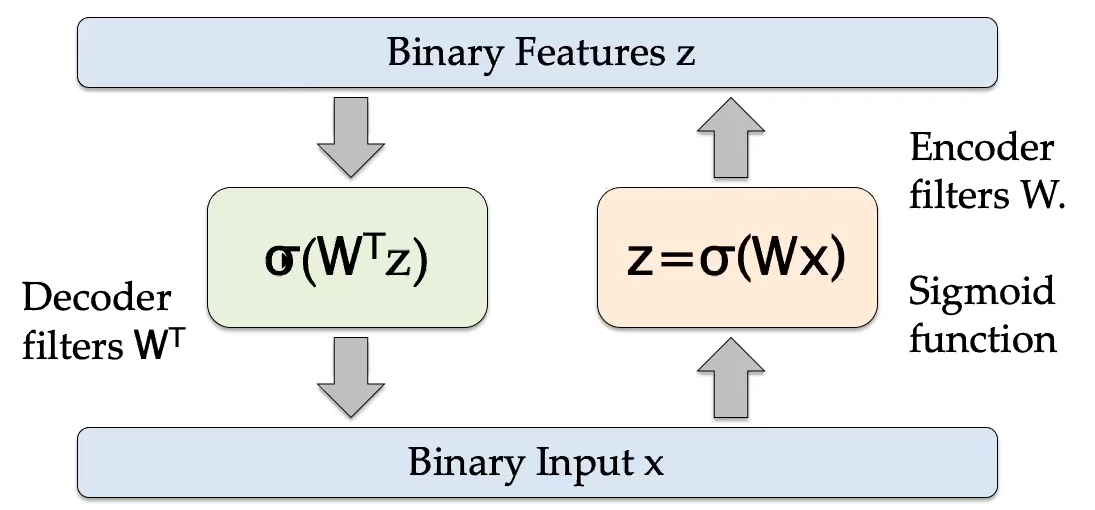
\includegraphics[scale=0.4]{Images/autoencoder_example.png}
\end{center}
where we have 
\begin{align*} 
    \mathrm{Encoder} & : \mathbf{h}(\mathbf{x}) = g(\mathbf{a}(x)) = \sigma (\mathbf{b} + \mathbf{W} \mathbf{x}) \\
    \mathrm{Decoder} & : \hat{\mathbf{a}}(\mathbf{x}) = \sigma (\mathbf{c} + \mathbf{W}^\ast \mathbf{h}(\mathbf{x})) 
\end{align*} 
The parameter gradients are obtained by backpropagating the gradient $\nabla_{\theta} \mathcal{L}$ like a regular network, but if we force tied weights (i.e. $W^\ast = W^T$), then $\nabla_{\mathbf{W}} \mathcal{L}$ is the sum of two gradients. This is because $\mathbf{W}$ is present both in the encoder and decoder. 

There are three things we can do to extract meaningful hidden features: 
\begin{enumerate}
    \item \textbf{Undercomplete Representation}: Make the latent dimension small. It compresses the input, but it may only be good for the training distribution and may not be robust to other types of input. If it is overcomplete, there is no guarantee that we will extract meaningful features. 
\item \textbf{Denoising Autoencoder}: Injecting noise to the input. The idea is that the representation should be robust to the introduction of noise. We take the original input $\mathbf{x}$ and we randomly assign a subset of the inputs to $0$, with probability $\nu$, similar to dropout, to get our noisy input $\Tilde{\mathbf{x}}$. Then we train the autoencoder with the loss comparing the output $\hat{\mathbf{x}}$ to the original, un-noisy input $\mathbf{x}$. We can do this for Gaussian additive noise too. As the visual below suggests, we are essentially ``pushing" out inputs away from the manifold and training the autoencoder to denoise it, pulling it back. 
    \begin{center}
        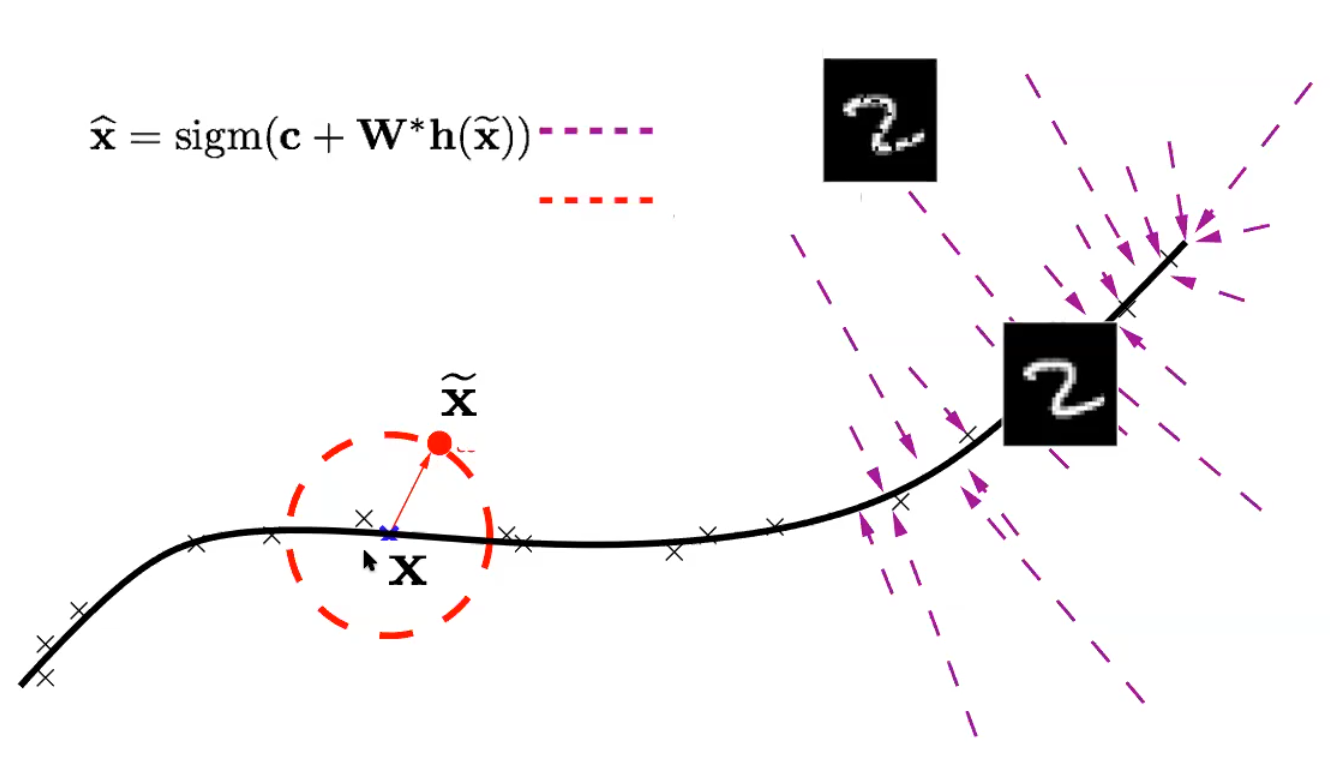
\includegraphics[scale=0.3]{Images/denoising_autoencoder.png}
    \end{center}
 
    \item \textbf{Contractive Autoencoder}: If we have the latent dimension greater than the input, then we can just add an explict term in the loss that penalizes that solution (e.g. promoting sparsity). For example, we can have the loss be 
    \[\mathcal{L}(f(\mathbf{x}^{(t)}) + \lambda || \nabla_{\mathbf{x}^{(t)}} \mathbf{h}(\mathbf{x}^{(t)})||^2_F\]
    where 
    \[||\nabla_{\mathbf{x}^{(t)}} \mathbf{h}(\mathbf{x}^{(t)})||_F^2 = \sum_{j, k} \bigg(\frac{\partial h(\mathbf{x}^{(t)})_j}{\partial x_k^{(t)}} \bigg)^2\]
    which forces the encoder to throw away information. If one of the elements are $0$, then we know that the $k$th element of the input has no effect on the $j$th element of the encoded output. Therefore, it tries to throw away as many elements of $\mathbf{x}$ as possible since the identity matrix will have a large Frobenius norm, essentially contracting the input representation.  

    We can also promote sparsity by adding a L1 penalty, forcing the feature space to be sparse. 
\end{enumerate}

The \textbf{predictive sparse decomposition} shows that the loss should be 
\[\min_{W, W^\ast, \mathbf{z}} ||W^\ast \mathbf{z} - \mathbf{x}||^2_2 + \lambda | \mathbf{z}|_1 + ||\sigma(W \mathbf{x}) - \mathbf{z}||^2_2\]
where the first term tells the decoder to reconstruct the original input well, the second tells the latent vector to be sparse, and the third tells us that we shouldn't lose too much information when we encode. 

We could also have \textbf{stacked autoencoders}, with each layer of latent features having some desired sparsity. 



\section{Boltzmann Machines} 

\subsection{Graphical Models}
 
Graphical models allow a nice way to represent complex probability distributions with some dependence relationship. 

\subsubsection{Directed Graphical Models}


\begin{definition}[Directed Probability Graph]  
A \textbf{probability graph} is a directed acyclic graph of $M$ nodes representing a joint probability distribution of $M$ scalar random variables. An edge pointing $A \rightarrow B$ means that the $B$ is conditionally dependent on $A$, and that there is a very clear casual relationship coming from $A$ to $B$. 
\begin{center}

\end{center}
The \textbf{parents} of a node $x_i$ is denoted $\mathrm{pa}_i$, and the entire joint distribution can be broken up as such: 
\[p(\mathbf{x}) = \prod_{m=1}^M p(x_m \mid x_{\mathrm{pa}_m})\]
\end{definition}


\begin{example}[Relay Race]

\end{example} 


Bayesian modelling with hierarchical priors. 

\begin{definition}[Ancestral Sampling] 
We can sample from the joint distribution by sequentially sampling starting from the parents to the final children, and discarding the ones (marginalizing) that we don't wish to sample. 
\end{definition}


\begin{example}
We first provide some motivation from a computational complexity perspective. Given a joint distribution of 2 random variables $\mathbf{x}_1, \mathbf{x}_2$, say which are multinomial with $K$ classes, their joint distribution $p(\mathbf{x}_1, \mathbf{x}_2)$ is captured by $K^2 - 1$ parameters. For a general $M$ random variables, then we have to keep a total of $K^M - 1$ parameters, and this increases exponentially. 
\begin{center}

\end{center}
By building a directed graph with say $r$ maximum number of variables appearing on either side of the conditioning bar in a single probability distribution, then the computational complexity scales as $O(K^r)$, which may save a lot of effort if $r << M$. 
\end{example}

Extending upon this example, we can see that we want to balance two things: 
\begin{enumerate} 
    \item Fully conncted graphs have completely general distributions and have $O(K^M -1)$ number of parameters (too complex). 
    \item If there are no links, the joint distribution fully factorizes into the product of its marginals and has $M(K-1)$ parameters (too simple) . 
\end{enumerate}
Graphs that have an intermediate level of connectivity allow for more general distributions compared to the fully factorized one, while requiring fewer parameters than the general joint distribution. One model that balances this out is the hidden markov model. 

\begin{example}[Chain Graph]
    Consider an $M$-node Markov chain. The marginal distribution $p(\mathbf{x}_1)$ requires $K-1$ parameters, and the remaining conditional distributions $p(\mathbf{x}_i \mid \mathbf{x}_{i-1})$ requires $K(K-1)$ parameters. Therefore, the total number of parameters is 
\[K-1 + (M-1) (K-1) K \in O(M K^2)\]
which scales relatively well, and we have 
\[p(\{\mathbf{x}_m\}) = p (\mathbf{x}_1) \prod_{m=2}^M p(\mathbf{x}_m \mid \mathbf{x}_{m-1})\]
\begin{center}

\end{center}
We can turn this same graph into a Bayesian model by introducing priors for the paramters. Therefore, each node requires an additional parent representing the distribution over parameters (e.g. prior can be Dirichlet)  
\[p(\{\mathbf{x}_m , \mu_m\}) = p(\mathbf{x}_1 \mid \mu_1) p(\mu_1) \prod_{m=2}^M p(\mathbf{x}_m \mid \mathbf{x}_{m-1}, \mu_m) p(\mu_m) \]
with $p(\mu_m) = \mathrm{Dir}(\mu_m \mid \alpha_m)$ for some predetermined fixed hyperparameter $\alpha_m$. 
\begin{center}
    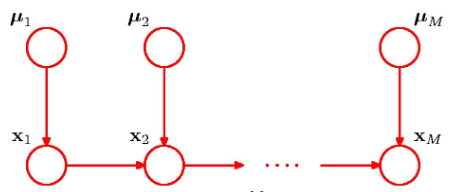
\includegraphics[scale=0.5]{Images/dir_prior.png}
\end{center}
We could also choose to share a common prior over the parameters, trading flexibility for computational feasibility. 
\begin{center}
    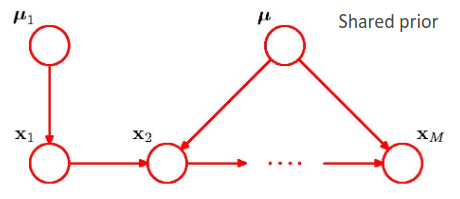
\includegraphics[scale=0.5]{Images/shared_dir_prior.png}
\end{center}
\end{example}

Another way to make more compact representations is through parameterized models. For example, if we have to compute $p(y = 1 \mid \mathbf{x}_1, \ldots, \mathbf{x}_M)$, this in general has $O(K^M)$ parameters. However, we can obtain a more parsimonious form by using a logistic function acting on a linear combination of the parent variables 
\[p(y = 1 \mid \mathbf{x}_1, \ldots, \mathbf{x}_m) = \sigma \bigg( w_0 + \sum_{i=1}^M w_i x_i \bigg) = \sigma(\mathbf{w}^T \mathbf{x}) \]
We can look at an example how this is applied to sampling from high-dimensional Gaussian with \textbf{linear Gaussian models}.  


\begin{example}[Multivariate Gaussian]
Consider an arbitrary acyclic graph over $D$ random variables, in which eachnode represents a single continuous Gaussian distribution with its mean given by a linear function of its parents. 
\[p(x_i \mid \mathbf{pa}_i) = N \bigg( x_i \bigg| w_{ij} x_j + b_j, v_i \bigg) \]
Given a multivariate Gaussian, let us try to decompose it into a directed graph. The log of the joint distribution takes form 
\[\ln p(\mathbf{x}) = \sum_{i=1}^D \ln p(x_i \mid \mathrm{pa}_i) = - \sum_{i=1}^D \frac{1}{2 v_i} \bigg( x_i - \sum_{j \in \mathrm{pa}_i} w_{ij} x_j - b_i \bigg)^2 + \mathrm{const}\]
To compute the mean, we can see that by construction, every $x_i$ is dependent on its ancestors, so 
\[x_i = \sum_{j \in \mathrm{pa}_i} w_{ij} x_j + b_i + \sqrt{v_i} \epsilon_i, \;\; \epsilon_i \sim N(0, 1)\]
so by linearity of expectation, we have 
\[\mathbb{E}[x_i] = \sum_{j \in \mathrm{pa}_i} w_{ij} \mathbb{E}[x_j] + b_i\]
So again, we can start at the top of the graph and compute the expectation. To compute covariance, we can obtain the $i, j$th element of $\boldsymbol{\Sigma}$ with a recurrence relation: 
\begin{align*} 
    \Sigma_{ij} & = \mathbb{E}[ (x_i - \mathbb{E}[x_i]) (x_j - \mathbb{E}[x_j])] \\
                & = \mathbb{E} \bigg[ (x_i - \mathbb{E}[x_i]) \bigg( \sum_{k \in \mathrm{pa}_j} w_{j k} (x_k - \mathbb{E}[x_k])  + \sqrt{v_i} \epsilon_j\bigg) \bigg] \\
                & = \sum_{k \in \mathrm{pa}_j} w_{j k} \Sigma_{ik} + I_{ij} v_j
\end{align*}
If there were no links in the graphs, then the $w_{ij}$'s are $0$, and so $\mathbb{E}[\mathbf{x}] = [b_1, \ldots, b_D]$, making the covariance diagonal.If the graph is fully connected, then the total number of parameters is $D + D(D-1)/2$, which corresponds to a general symmetric covariance matrix.  
\end{example}

\begin{example}[Bilinear Gaussian Model]
Consider the following model
\begin{align*}
    u & \sim N(0, 1) \\
    v & \sim N(0, 1) \\
    r & \sim N(u v, 1)
\end{align*}
where the mean of $r$ is a product of $2$ Gaussians. This is also a parameterized model. 
\begin{center}
    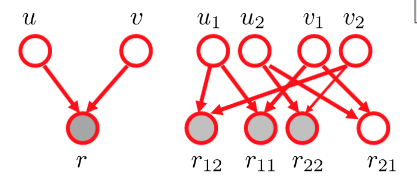
\includegraphics[scale=0.6]{Images/bilinear_gaussian.png}
\end{center}
\end{example}

\begin{definition}[Conditional Independence in Directed Graphs]
We say that $a$ is independent of $b$ given $c$ if 
\[p(a \mid b, c) = p(a \mid c)\]
or equivalently, 
\[p(a, b \mid c) = p(a \mid b, c)\, p(b \mid c) = p(a \mid c) \, p(b \mid c)\]
Conveniently, we can directly read conditional independence properties of the joint distribution from the graph without any analytical measurements. 
\end{definition}

\begin{example}
    We can demonstrate conditional independence with iid data. Consider the problem of density estimation of some dataset $\mathcal{D} = \{x_i\}$ with some parameterized distribution of $\mu$. As shown below, if we condition on $\mu$ and considered the joint over the observed variables, the variables are independent, but if we integrate out $\mu$, the observations are no longer independent. 
\begin{center}
    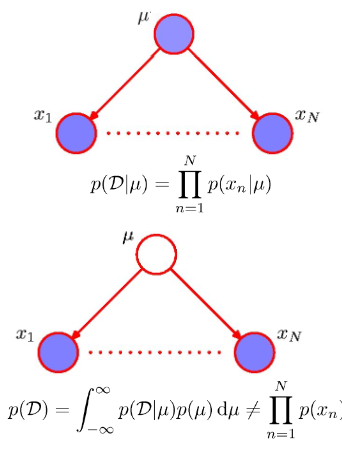
\includegraphics[scale=0.6]{Images/iid_conditional_independence.png}
\end{center}
\end{example}

The example above identifies a node (the parent $\mu$) where, if observed, causes the rest of the nodes to become independent. We can extend on this idea by taking an arbitrary $x_i$ and finding a set of nodes such that if they are observed, then $x_i$ is indepedent from every other node. 

\begin{definition}[Markov Blanket]
    The \textbf{Markov blanket} of a node is the minimal set of nodes that must be observed to make this node independent of all other nodes. It turns out that the parents, children, and coparents are all in the Markov blanket. 
\begin{center}
    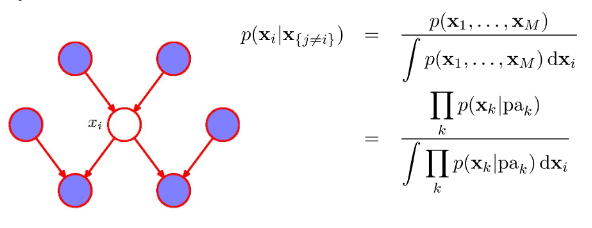
\includegraphics[scale=0.6]{Images/markov_blanket.png} 
\end{center}
\end{definition} 

One final interpretation is that we can view directed graphs as \textbf{distribution filters}. We take the joint probability distribution, will starts off as fully connected, and the directed graphs ``filters" away the edges that are not needed. Therefore, the joint probability distribution $p(\mathbf{x})$ is only allows through the filter if and only if it satisfies the factorization property. 

\subsubsection{Undirected Graphical Models}

As the name implies, undirected models use undirected graphs, which are used to model relationships that go both ways rather than just one. Unlike directed graphs, which are useful for expressing casual relationships between random variables, undirected graphs are useful for expressing soft constraints between random variables.  

\begin{definition}[Conditional Independence in Undirected Graphs]
Fortunately, conditional independence is easier compared to directed models. We can say $A$ is conditionally independent to $B$ given $C$ if $C$ blocks all paths between any node in $A$ and any node in $B$. 
\begin{center}
    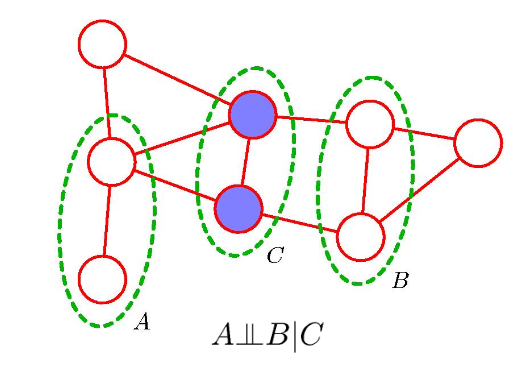
\includegraphics[scale=0.4]{Images/conditional_independence_undirected.png}
\end{center}
\end{definition}

\begin{definition}[Markov Blanket in Undirected Graphs]
The Markov blanket of a node, which is the minimal set of nodes that must be observered to make this node independent of the rest of the nodes, is simply the nodes that are directly connected to that node. 
\begin{center} 
    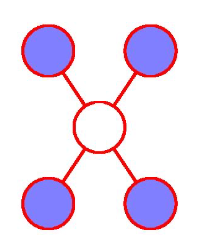
\includegraphics[scale=0.4]{Images/markov_blanket_undirected.png}
\end{center}
Therefore, the conditional distribution of $x_i$ conditioned on all the variables in the graph is dependent only on the variables in the Markov blanket. 
\end{definition}

Now, let us talk about how we can actually define a probability distribution with this graph. 


\begin{definition}[Clique] 
    In an undirected graph, a \textbf{clique} is a set of nodes such that there exists a link between all pairs of nodes in that subset. A \textbf{maximal clique} is a clique such that it is not possible to include any other nodes in the set without it ceasing it to be a clique. 
\end{definition}

Given a joint random variable $\mathbf{x}$  represented by an undirected graph, the joint distribution is given by the product of non-negative potential functions over the maximal cliques 
\[p(\mathbf{x}) = \frac{1}{Z} \prod_C \phi_C (x_C)\] 
where 
\[Z = \int p(\mathbf{x}) \,d\mathbf{x}\] 
is the normalizing constant, called the \textbf{partition function}. That is, each $x_C$ is a maximal clique and $\phi_C$ is the nonnegative potential function of that clique. 

This assignment looks pretty arbitrary. How do we know that any arbitrary joint distribution of $\mathbf{x}$, which has a undirected graphical representation, can be represented as the product of a bunch of functions over the maximum cliques? Fortunately, there is a mathematical result that proves this. 

\begin{theorem}[Hammersley-Clifford] 
The joint probability distribution of any undirected graph can be written as the product of potential functions on the maximal cliques of the graph. Furthermore, for any factorization of these potential functions, there exists an undirected graph for which is the joint.  
\end{theorem} 


\begin{example}
For example, the joint distribution of the graph below
\begin{center}
    \includegraphics[scale=0.5]{Images/clique_factor.png}
\end{center}
factorizes into 
\[p(A, B, C, D) = \frac{1}{Z} \phi(A, C) \, \phi(C, B) \, \phi(B, D) \, \phi(A, D)\]
\end{example}

Note that each potential function $\phi$ is a mapping from the joint configuration of random variables in a clique to non-negative real numbers. The choice of potential functions is not restricted to having specific probabilistic interpretations, but since they must be nonnegative, we can just represent them as an exponential. The negative sign is not needed, but is a remnant of physics notation. 
\[p (\mathbf{x}) = \frac{1}{Z} \prod_C \phi_C (x_C) = \frac{1}{Z} \exp \bigg\{ - \sum_C E(x_C) \bigg\} = \frac{1}{Z} \underbrace{\exp \big\{ - E(\mathbf{x}) \big\}}_{\substack{\text{Boltzmann}\\ \text{distribution}}}\]

Any distribution that can be represented as the form above is called a \textbf{Boltzmann distribution}. So far, all we stated is that the joint probability distribution can be expressed as the product of a bunch of potential functions, but besides the fact that it is nonnegative, there is no probabilistic interpretation of these potentials (or equivalently, the energy functions). While this does give us greater flexibility in choosing potential functions, we must be careful in choosing them (e.g. choosing something like $x^2$ may cause the integral to diverge, making the joint not well-defined).

Clearly, these potential functions over the cliques should express which configuration of the local variables are preferred to others. It should assign higher values to configurations that are deemed (either by assumption or through training data) to be more probable. That is, each potential is like an ``expert" that provides some opinion (the value) on a configuration, and the product of the values of all the potential represents the total opinion of all the experts. Therefore, global configurations with relatively high probabilities are those that find a good balance in satisfying the (possibly conflicting) influences of the clique potentials. 

\begin{example}[Transmission of Colds] 
Say that you want to model a distribution over three binary variables: whether you or not you, your coworker, and your roommate is sick ($0$ represents sick and $1$ represents healthy). Then, you can make simplifying assumptions that your roommate and your coworker do not know each other, so it is very unlikely that one of thme will give the other an infection such as a cold directly. Therefore, we can model the indirect transmission of a cold from your coworker to your roommate by modeling the transmission of the cold from your coworker to you and then you to your roommate. Therefore, we have a model of form

\begin{center}
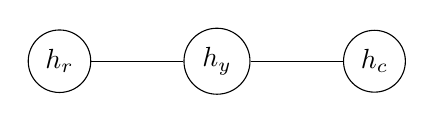
\begin{tikzpicture}
    \node[circle,draw] (hr) at (0,0) {$h_r$};
    \node[circle,draw] (hy) at (2,0) {$h_y$};
    \node[circle,draw] (hc) at (4,0) {$h_c$};

    \draw (hr) -- (hy);
    \draw (hy) -- (hc);
\end{tikzpicture}
\end{center}
One max clique contains $h_y$ and $h_c$. The factor for this clique can be defined by a table and might have values resembling these. 
\begin{table}[h]
\centering
\begin{tabular}{c|c|c|}
\cline{2-3}
& \( h_y = 0 \) & \( h_y = 1 \) \\ \hline
\multicolumn{1}{|c|}{\( h_c = 0 \)} & 2 & 1 \\ \hline
\multicolumn{1}{|c|}{\( h_c = 1 \)} & 1 & 10 \\ \hline
\end{tabular}
\caption{States and Values of \( h_y \) and \( h_c \)}
\end{table}
This table completely describes the potential function of this clique. Both of you are usually healthy, so the state $(1, 1)$ gets the maximum value of $1$. If one of you are sick, then it is likely that the other is sick as well, so we have a value of $2$ for $(0, 0)$. Finally, it is most unlikely that one of you is sick and the other healthy, which has a value of $1$. 
\end{example}

\subsection{Boltzmann Machines} 

Now that we've learned about graphical models, let's put them to use. We have some unknown joint distribution $\mathbf{x}$, and we want to represent it in a graph such that it is not too computationally hard to calculate probabilities and sample from them, but at the same time not so simple such that it doesn't richly capture a broad family of probability distributions. One architecture is to use \textbf{Markov Random Fields}, which represent these joint distributions with undirected graphs satisfying the Markov properties. 

The Hammersley-Clifford theorem states that the joint PDF of any MRF can be written a a Boltzmann distribution. For now, we will limit outselves to \textbf{parwise MRFs}, which only capture dependencies between cliques of maximum size $2$. For example, a MRF can be represented with the graph $G(V, E)$ below. 
\begin{center}
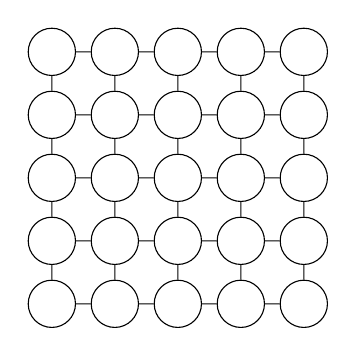
\begin{tikzpicture}[scale=0.8]
  % Define nodes in a 5x5 grid
  \foreach \i in {1,...,5} {
    \foreach \j in {1,...,5} {
      \node[circle, draw, minimum size=0.6cm] (node\i\j) at (\i, \j) {};
    }
  }

  % Connect nodes like an Ising model
  \foreach \i in {1,...,5} {
    \foreach \j in {1,...,5} {
      \pgfmathtruncatemacro{\right}{\i+1}
      \pgfmathtruncatemacro{\down}{\j-1}
      \pgfmathtruncatemacro{\up}{\j+1}
      \pgfmathtruncatemacro{\left}{\i-1}
      
      \ifnum \i < 5
        \draw (node\i\j) -- (node\right\j);
      \fi
      
      \ifnum \j > 1
        \draw (node\i\j) -- (node\i\down);
      \fi
    }
  }
\end{tikzpicture}
\end{center}



\begin{definition}[Bernoulli Pairwise Markov Random Fields]
    MRFs with binary variables are sometimes \textbf{Ising models} in statistical mechanics, and \textbf{Boltzmann machines} in machine learning. By Hammersley-Clifford, we don't even need to specify the individual functions over the maximal cliques, and rather we can just specify the energy function $E(\mathbf{x})$ of the Boltzmann distribution that the MRF encodes. We define it to capture the interactions between random variables $x_i$ up to order $2$. 
\[p_{\boldsymbol{\theta}} (\mathbf{x}) = \frac{1}{Z} \exp \bigg( \sum_{ij \in E} x_i x_j \theta_{ij} + \sum_{i \in V} x_i \theta_i \bigg) \]
Now let's check its conditional distribution. 
\begin{align*}
    p(x_k = 1 \mid \mathbf{x}_{-k}) & = \frac{p(x_k = 1, \mathbf{x}_{-k})}{p(\mathbf{x}_{-k})} \\
                                    & = \frac{p(x_k = 1, \mathbf{x}_{-k})}{p(x_k = 0, \mathbf{x}_{-k}) + p(x_k = 1, \mathbf{x}_{-k})} \\
                                    & = \frac{\exp \Big( \sum_{k j \in E} x_j \theta_{kj} + x_k \theta_k \Big)}{\exp(0) + \exp \Big(\sum_{k j \in E} x_j \theta_{kj} + x_k \theta_k \Big)} \\
                                    & = \sigma \bigg\{ - \theta_k x_k - \sum_{k j \in E} x_j \theta_{k j} \bigg\} 
\end{align*}
where the penultimate step comes from evaluating 
\begin{align*} 
    p(x_k = 1, \mathbf{x}_{-k}) & = \frac{1}{Z(\boldsymbol{\theta})} \exp \bigg( \sum_{ij \in E, k \neq i, j} x_i x_j \theta_{ij} + \sum_{i j \in E, k = i, j} x_i x_j \theta_{ij} + \sum_{i \in V, i \neq k} x_i \theta_i + x_k \theta_k \bigg) \\
                                & =\frac{1}{Z(\boldsymbol{\theta})} \exp \bigg( \sum_{ij \in E, k \neq i, j} x_i x_j \theta_{ij} + \sum_{k j \in E} x_j \theta_{kj} + \sum_{i \in V, i \neq k} x_i \theta_i + \theta_k \bigg)  \\ 
    p(x_k = 0, \mathbf{x}_{-k}) & = \frac{1}{Z(\boldsymbol{\theta})} \exp \bigg( \sum_{ij \in E, k \neq i, j} x_i x_j \theta_{ij} + \sum_{i \in V, i \neq k} x_i \theta_i\bigg)  
\end{align*}
and canceling out like terms in the numerator and denominator. This tells us that MRFs are related to logistic function.  
\end{definition}

We have given our first example of a Boltzmann machine. Let's generalize this a little bit by removing the restriction that there can only be pairwise connections. Then, we can model the second order interactions with the slightly more generalized energy function
\[E(\mathbf{x}) = -\mathbf{x}^T \mathbf{U} \mathbf{x} - \mathbf{b}^T \mathbf{x}\]
Now this slightly expands the coverage of probability distributions given our model, and we can see that this allows us to model Gaussian distributions. 

\begin{example}[Gaussian Markov Random Fields] 
    If we assume that $p_{\boldsymbol{\theta}} ( \mathbf{x})$ folows a multivariate Gaussian distribution, we have 
\[p(\mathbf{x} \mid \boldsymbol{\mu}, \boldsymbol{\Sigma}) = \frac{1}{Z} \exp \bigg( -\frac{1}{2} (\mathbf{x} - \boldsymbol{\mu})^T \boldsymbol{\Sigma}^{-1} (\mathbf{x} - \boldsymbol{\mu}) \bigg)\]
Since the Gaussian distribution reprsents at most second-order relationships, it automatically encodes a pairwise MRF. Therefore, we can rewrite 
\[p(\mathbf{x}) = \frac{1}{Z} \exp \bigg( -\frac{1}{2} \mathbf{x}^T J\mathbf{x} + \mathbf{g}^T \mathbf{x} \bigg)\] 
where $J = \boldsymbol{\Sigma}^{-1}$ and $\boldsymbol{\mu} = J^{-1} \mathbf{g}$. 
\end{example}

Let's review what we had so far. There is a random vector $\mathbf{x}$ for which we would like to model the probability distribution of. 

\begin{center}
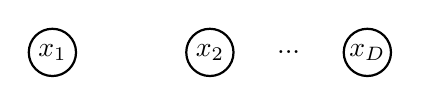
\begin{tikzpicture}
  % Define the nodes
  \node (x1) at (0,0) {$x_1$};
  \node (x2) at (2,0) {$x_2$};
  \node (xD) at (4,0) {$x_D$};

  % Add the "..." text box
  \node at (3,0) {...};
  \draw[thick] (x1) circle (0.3);
  \draw[thick] (x2) circle (0.3);
  \draw[thick] (xD) circle (0.3);
\end{tikzpicture}
\end{center}

What we can do is model the dependencies between these random elements with linear parameters $\mathbf{W}$ and $\mathbf{b}$, which essentially gives us a Markov Random Field.  

However, this is still quite a limited model. For one, due to the linearity of the weight matrix, it always turns out that the probability of $x_k = 1$ is always given by a linear model (logistic regression) from the values of the other units. This family of distributions parameterized by $\boldsymbol{\theta} = \{\mathbf{W}, \mathbf{b}\}$ may not be broad enough to capture the true $p(\mathbf{x})$. Therefore, we can add latent variables that can act similarly to hidden uits in a MLP and model higher-order interactions among the visible units. Just as the addition of hidden units to convert logistic regression into MLP results in the MLP being a universal approximator of functions, a Boltzmann machine with hidden units is not longer limited to modeling linear relationships between variables. Instead, the Boltzmann machine becomes a universal approximator of probability mass functions over discrete random variables. 

\begin{definition}[Boltzmann Machine]
    The original \textbf{Boltzmann machine} has the energy function 
\[E(\mathbf{v}, \mathbf{h}) = - \mathbf{v}^T \mathbf{R} \mathbf{v} - \mathbf{v}^T \mathbf{W} \mathbf{h} - \mathbf{h}^T \mathbf{S} \mathbf{h} - \mathbf{b}^T \mathbf{v} - \mathbf{c}^T \mathbf{h} \]
It can represent the undirected graph that has connections within the $\mathbf{x}$, within the $\mathbf{h}$, and between the $\mathbf{x}$ and $\mathbf{h}$.
\begin{center} 
    \includegraphics[scale=0.4]{Images/Boltzmann_lateral.png}
\end{center}
Therefore, by adding latent variables and connecting everything together, this gives us a very flexible model that can capture a lot of distribtions.
\end{definition} 

 \subsubsection{Restricted Boltzmann Machines} 

\begin{definition}[Restricted Boltzmann Machine] 
    Now, if we put a restriction saying that there cannot be any intra-connections in the $\mathbf{x}$ and $\mathbf{h}$, then we get the \textbf{restricted Boltzmann machine}, which has a slightly more resticted form of the energy function than the general BM. The probability distributions that it can model has a graph that looks like 
\begin{center}
    \includegraphics[scale=0.4]{Images/rbm_layer.png}
\end{center}
with connections only allowed between $x_i$'s and $h_j$'s, known as a \textbf{bipartite graph}, implying that the maximum clique length is $2$. This model allows the elements of $\mathbf{x}$ to be dependent, but this architecture allows for \textit{conditional independence}, and not just for $\mathbf{x}$ given $\mathbf{h}$, but also $\mathbf{h}$ given $\mathbf{x}$. Therefore, we already have the extremely nice property that 
\begin{align*} 
    p(\mathbf{x} \mid \mathbf{h}) & = \prod_{k=1}^{D} p(x_k \mid \mathbf{h}) \\
    p(\mathbf{h} \mid \mathbf{x}) & = \prod_{j=1}^F p(h_j \mid \mathbf{x}) 
\end{align*}
\end{definition}

The fact that we can calculate $p(\mathbf{h} \mid \mathbf{x})$ means that inferring the distribution over the hidden variables is easy. Keep in mind that there are three architectures we've talked about: 
\begin{enumerate}
    \item Markov Random Fields, which model just the original $\mathbf{x}$. 
    \item Restricted Boltzmann machines, which models $\mathbf{x}, \mathbf{h}$ and not allowing intra-connections. 
    \item Boltzmann machines, which models $\mathbf{x}, \mathbf{h}$. Boltzmann machines without latent variables are just MRFs.  
\end{enumerate}

\begin{definition}[Bernoulli-Bernoulli RBM]
    For now, let us assume that we are trying to estimate the distribution of a Bernoulli random vector $\mathbf{x} \in \{0, 1\}^D$ with Bernoulli latent variables $\mathbf{h} \in \{0, 1\}^F$. Then, the energy of the joint configuration is  
\[E(\mathbf{v}, \mathbf{h}; \boldsymbol{\theta}) = - \sum_{ij} W_{ij} v_i h_j - \sum_i b_i v_i - \sum_j a_j h_j = - \mathbf{v}^T \mathbf{W} \mathbf{h} - \mathbf{b}^T \mathbf{v} - \mathbf{a}^T \mathbf{h}\]
where $\boldsymbol{\theta} = \{\mathbf{W}, \mathbf{a}, \mathbf{b}\}$ are the model parameters. So we have 
\begin{align*} 
    p_{\boldsymbol{\theta}} (\mathbf{v}, \mathbf{h}) & = \frac{1}{Z} \exp \big( -E (\mathbf{v}, \mathbf{h}; \boldsymbol{\theta})\big) = \frac{1}{Z} \prod_{ij} e^{W_ij v_i h_j} \prod_i e^{b_i v_i} \prod_j e^{a_j h_j} \\
    Z & = \sum_{\mathbf{h}, \mathbf{v}} \exp \big( -E(\mathbf{v}, \mathbf{h}; \boldsymbol{\theta}) \big) 
\end{align*}
where we can think of the $\exp(\mathbf{h}^T \mathbf{W} \mathbf{x})$ as encoding the cliques of length $2$ and the others as cliques of length $1$.  
\end{definition}

Let's get some calculations out of the way. 

\begin{lemma}[Conditional Distributions] 
For the Bernoulli RBM, we have 
\begin{align*} 
    p(h_j = 1 \mid \mathbf{x}) & = \sigma ( b_j + W_{j,:} \mathbf{x}) \\
    p(x_k = 1 \mid \mathbf{h}) & = \sigma ( c_k + \mathbf{h}^T \mathbf{W}_{:, k})
\end{align*}
\end{lemma}
\begin{proof}
Just use the definition of conditional probability and substitute the result below in the denominator. The terms will cancel out. 
\end{proof}


\begin{lemma}[Free Energy] 
    For the Bernoulli RBM, we want to compute the marginal $p(\mathbf{x})$ as
\begin{align*} 
    p(\mathbf{x}) & = \frac{\exp(-F(\mathbf{x}))}{Z} \\
                  & = \frac{1}{Z} \exp \bigg( \mathbf{c}^T \mathbf{x} + \sum_{j=1}^H \log \big( 1 + \exp (b_j + \mathbf{W}_{j, :} \mathbf{x}) \big) \bigg) \\
                  & = \frac{1}{Z} \exp \bigg( \mathbf{c}^T \mathbf{x} + \sum_{j=1}^H \mathrm{softplus}(b_j + W_{j, :} \mathbf{x} ) \bigg)
\end{align*}
where $F$ is called the \textbf{free energy}. Therefore, $p(\mathbf{x})$ is calculated by taking the product of these terms, which is why it's known as a \textbf{product of experts model}. 
\begin{center}
    \includegraphics[scale=0.4]{Images/softplus.png} 
\end{center}
\end{lemma}
\begin{proof}
We have 
\begin{align*} 
    p(\mathbf{x}) & = \sum_{\mathbf{h} \in \{0, 1\}^H} \exp \big( \mathbf{h} \mathbf{W} \mathbf{x} + \mathbf{c}^T \mathbf{x} + \mathbf{b}^T \mathbf{h}\big) /Z \\
                  & = \exp (\mathbf{c}^T \mathbf{x}) \sum_{h_1 = 0, 1} \ldots \sum_{h_H = 0, 1} \exp \bigg( \sum_j h_j \mathbf{W}_{j, :} \mathbf{x} + b_j h_j \bigg) / Z \\
                  & = \exp (\mathbf{c}^T \mathbf{x}) \bigg( \sum_{h_1 = 0, 1} \exp (h_1 \mathbf{W}_{1, :} \mathbf{x} + b_1 h_1 ) \bigg) \ldots \bigg( \sum_{h_H = 0, 1} \exp (h_H \mathbf{W}_{H, :} \mathbf{x} + b_H h_H) \bigg) / Z \\
                  & = \exp (\mathbf{c}^T \mathbf{x}) \big( 1 + \exp (b_1 + \mathbf{W}_{1, :} \mathbf{x}) \big) \ldots \big( 1 + \exp (b_H + \mathbf{W}_{H, :} \mathbf{x})\big) / Z \\
                  & = \exp (\mathbf{c}^T \mathbf{x}) \exp\big\{ \log \big( 1 + \exp (b_1 + \mathbf{W}_{1, :} \mathbf{x}) \big) \big\} \ldots \exp \big\{ \log \big( 1 + \exp (b_H + \mathbf{W}_{H, :} \mathbf{x}) \big) \big\} / Z \\
                  & = \frac{1}{Z} \exp \bigg( \mathbf{c}^T \mathbf{x} + \sum_{j=1}^H \log \big( 1 + \exp (b_j + \mathbf{W}_{j, :} \mathbf{x}) \big) \bigg) 
\end{align*} 
\end{proof}

Now that we've done this, we can finally get to training the model. Now, essentially this is density estimation problem given dataset $\mathcal{D} = \{\mathbf{x}^{(t)}\}$ of iid random variables, we want to maximize the likelihood of $p_{\boldsymbol{\theta}}$, which is really just equivalent to optimizing $E_{\boldsymbol{\theta}}$. So, let's take the average negative log-likelihood and take the derivative of it
\[\frac{\partial}{\partial \boldsymbol{\theta}} \frac{1}{T} \sum_t - \log p_{\boldsymbol{\theta}} (\mathbf{x}^{(t)}) = \frac{1}{T} \sum_t - \log{p_{\boldsymbol{\theta}} (\mathbf{x}^{(t)})}\]
There's a lot of computation to do here, so let's focus on one sample $\mathbf{x}^{(t)}$ and claim that the gradient ultimately ends up as the following. 

\begin{theorem}
It turns out that
\begin{align*} 
    \frac{\partial}{\partial \boldsymbol{\theta}} - \log p(\mathbf{x}^{(t)}) & = \sum_{\mathbf{h}}  p(\mathbf{h} \mid \mathbf{x}^{(t)}) \, \frac{ \partial E(\mathbf{x}^{(t)}, \mathbf{h})}{\partial \boldsymbol{\theta}} - \sum_{\mathbf{x}, \mathbf{h}} p(\mathbf{x}, \mathbf{h}) \, \frac{\partial E(\mathbf{x}, \mathbf{h})}{\partial \boldsymbol{\theta}} \\
                                                                             & = \mathbb{E}_{\mathbf{h}} \bigg[ \frac{\partial E( \mathbf{x}^{(t)}, \mathbf{h})}{\partial \boldsymbol{\theta}} \; \bigg| \; \mathbf{x}^{(t)} \bigg] - \mathbb{E}_{\mathbf{x}, \mathbf{h}} \bigg[ \frac{\partial E(\mathbf{x}, \mathbf{h})}{\partial \boldsymbol{\theta}} \bigg]  
\end{align*}
The derivative of $E$ is easy since we already know the bilinear form by construction. In the left term, we are taking the expectation w.r.t. $p(\mathbf{h} \mid \mathbf{x}^{(t)})$, which we can factorize out due to conditional independence, so this is easy. However, the right term requires us to integrate over the joint $p(\mathbf{x}, \mathbf{h})$, which is intractable, and so we just approximate this with a Monte Carlo sample. 
\end{theorem}
\begin{proof}
As a lemma, we first see that $\ln(Z) = \ln \big( \sum_{\mathbf{x}, \mathbf{h}} \exp \big( - E(\mathbf{x}, \mathbf{h}) \big) \big)$, and so
\[\frac{\partial \ln(Z)}{\partial \boldsymbol{\theta}} = -\frac{1}{Z} \sum_{\mathbf{x}, \mathbf{h}} \exp \big(-E(\mathbf{x}, \mathbf{h})\big) \, \frac{E(\mathbf{x}, \mathbf{h})}{\partial \boldsymbol{\theta}} = - \sum_{\mathbf{x}, \mathbf{h}} p(\mathbf{x}, \mathbf{h}) \, \frac{\partial E(\mathbf{x}, \mathbf{h})}{\partial \boldsymbol{\theta}}\]
We have 
\begin{align*} 
    -\ln p(\mathbf{x}) & = - \ln \bigg\{ \sum_{\mathbf{h}} \exp \big( -E(\mathbf{x}, \mathbf{h}) \big) \bigg\} + \ln(Z)
\end{align*}
and so we can apply chain rule and multiply both numerator and denominator by $1/Z$ to get 
\begin{align*} 
    -\frac{\partial}{\partial \boldsymbol{\theta}} \ln p(\mathbf{x}) & = \frac{\sum_{\mathbf{h}} \exp \big( -E(\mathbf{x}, \mathbf{h}) \big) \, \frac{\partial E(\mathbf{x}, \mathbf{h})}{\partial \boldsymbol{\theta}} / Z}{\sum_{\mathbf{h}} \exp \big( -E (\mathbf{x}, \mathbf{h}) \big) / Z} + \frac{\partial \ln(Z)}{\partial \boldsymbol{\theta}} \\
                                                                     & = \frac{\sum_{\mathbf{h}} p(\mathbf{x}, \mathbf{h}) \, \frac{\partial E(\mathbf{x}, \mathbf{h})}{\partial \boldsymbol{\theta}}}{p(\mathbf{x})} + \frac{\partial \ln(Z)}{\partial \boldsymbol{\theta}} \\
                                                                     & = \sum_{\mathbf{h}} p(\mathbf{h} \mid \mathbf{x}) \, \frac{\partial E(\mathbf{x}, \mathbf{h})}{\partial \boldsymbol{\theta}} - \sum_{\mathbf{x}, \mathbf{h}} p(\mathbf{x}, \mathbf{h}) \, \frac{\partial E(\mathbf{x}, \mathbf{h})}{\partial \boldsymbol{\theta}} 
\end{align*}
\end{proof} 

So to calculate the second expectation, we can use a Gibbs sampler to do some numerical integration, but before we do that, let's just find the partial of $E$, which should be simple. 
\[\frac{\partial E(\mathbf{x}, \mathbf{h})}{\partial W_{j k}} = \frac{\partial}{\partial W_{j k}} \bigg( - \sum_{j k} W_{j k} h_j x_k - \sum_k c_k x_k - \sum_j b_j h_j \bigg) = h_j x_k\]
and so 
\[\mathbb{E}_{\mathbf{h}} \bigg[ \frac{\partial E(\mathbf{x}, \mathbf{h})}{\partial W_{j k}} \bigg| \mathbf{x} \bigg] = \mathbb{E}_{\mathbf{h}} [ -h_j x_k \mid \mathbf{x}] = \sum_{h_j = 0, 1} - h_j x_k \, p(h_j \mid \mathbf{x}) = - x_k p(h_j = 1 \mid \mathbf{x})\]
where the final term is a sigmoid. Hence, we have 
\[\mathbb{E}_{\mathbf{h}} [ \nabla_{\mathbf{W}} E(\mathbf{w}, \mathbf{h}) \mid \mathbf{x}] = - \mathbf{h}(\mathbf{x}) \mathbf{x}^T, \text{ where } \mathbf{h}(\mathbf{x}) \coloneqq \begin{pmatrix} p(h_1 = 1 \mid \mathbf{x}) \\ \vdots \\ p(h_H = 1 \mid \mathbf{x}) \end{pmatrix} = \sigma(\mathbf{b} + \mathbf{W} \mathbf{x}) \]
Now we can substitute what we solved into the second expectation, but again this is infeasible to calculate 
\[\mathbb{E}_{\mathbf{x}, \mathbf{h}} \bigg[ \frac{\partial E(\mathbf{x}, \mathbf{h})}{\partial\boldsymbol{\theta}}\bigg] = \sum_{\mathbf{x}, \mathbf{h}} \mathbf{h}(\mathbf{x}) \mathbf{x}^T p(\mathbf{x}, \mathbf{h}) \]
The way we do this is through \textbf{contrastive divergence}, which estimates the expectation through Gibbs sampling. Since we know $p(\mathbf{x}\mid \mathbf{h})$ and $p(\mathbf{h} \mid \mathbf{x})$ easily, we can start sampling the chain for some predetermined $K$ steps (actually $2K$ since we are sampling the $x$ and $h$ back and forth), and whatever $\bar{\mathbf{x}}$ you sample at the end is your estimate. So, once you should update your gradient, you start at the sample $\mathbf{x}^{(t)}$, run Gibbs for $k$ steps, and use that to estimate your gradient, and then move onto the next sample. We can tweak this procedure, such as \textbf{persistent CD}, where instead of initializing the chain to $\mathbf{x}^{(t)}$, we can initialize the chain to the negative sample of the last iteration. 
\begin{center}
    \includegraphics[scale=0.4]{Images/contrastive_divergence.png}
\end{center}
Therefore, for updating $\mathbf{W}$, we get the following 
\begin{align*} 
    \mathbf{W} & = \mathbf{W} - \alpha \big( \nabla_{\mathbf{W}}(- \log p(\mathbf{x}^{(t)})) \big) \\
               & = \mathbf{W} - \alpha \big( \mathbb{E}_{\mathbf{h}} [ \nabla_{\mathbf{W}} E(\mathbf{x}^{(t)}, \mathbf{h}) \mid \mathbf{x}^{(t)} ] - \mathbb{E}_{\mathbf{x}, \mathbf{h}} [\nabla_{\mathbf{W}} E(\mathbf{x}, \mathbf{h}) ]\big) \\
               & = \mathbf{W} - \alpha \big( \mathbb{E}_{\mathbf{h}} [ \nabla_{\mathbf{W}} E(\mathbf{x}^{(t)}, \mathbf{h}) \mid \mathbf{x}^{(t)} ] - \mathbb{E}_{\mathbf{h}} [\nabla_{\mathbf{W}} E(\bar{\mathbf{x}}, \mathbf{h}) \mid \bar{\mathbf{x}} ]\big) \\
               & = \mathbf{W} + \alpha \big( \mathbf{h}(\mathbf{x}^{(t)}) (\mathbf{x}^{(t)})^T               - \mathbf{h}(\bar{\mathbf{x}}) \bar{\mathbf{x}}^T \big)
\end{align*}
and doing this over all three parameters leads to 
\begin{align*} 
    \mathbf{W} & \leftarrow \mathbf{W} + \alpha \big( \mathbf{h} (\mathbf{x}^{(t)}) (\mathbf{x}^{(t)})^T - \mathbf{h}(\bar{\mathbf{x}}) \bar{\mathbf{x}}^T \big) \\
    \mathbf{b} & \leftarrow \mathbf{b} + \alpha \big( \mathbf{h}(\mathbf{x}^{(t)}) - \mathbf{h}(\bar{\mathbf{x}}) \big) \\
\mathbf{c} & = \leftarrow \mathbf{c} + \alpha \big( \mathbf{x}^{(t)} - \hat{\mathbf{x}} \big) 
\end{align*}
Therefore, contrastive divergence with $k$ iterations gives us the \textbf{CD-k algorithm}. In general, the bigger $k$ is, the less biased the estimate of the gradient will be, and in practice $k=1$ works well for learning good features. The reason this is called contrastive divergence is that in the gradient update step, we have a positive sample and a negative sample that both approximates the expected gradient, which constrasts to each other. 

\subsubsection{Gaussian Bernoulli RBMs}

\begin{definition}[Gaussian-Bernoulli RBM] 
If we assume that $\mathbf{v}$ is a real-valued (unbounded) input that follows a Gaussian distribution (with $\mathbf{h}$ still Bernoulli), then we can add a quadratic term to the energy function 
\[E(\mathbf{x}, \mathbf{h}) = - \mathbf{h}^T \mathbf{W} \mathbf{x} - \mathbf{c}^T \mathbf{x} - \mathbf{b}^T \mathbf{h} - \frac{1}{2} \mathbf{x}^T \mathbf{x}\]
In this case, $p(\mathbf{x} \mid \mathbf{h})$ becomes a Gaussian distribution $N(\mathbf{c} + \mathbf{W}^T \mathbf{h}, \mathbf{I})$. The training process is slightly harder for this, so what we usually do is normalize the training set by subtracting the mean off each input and dividing the input by the training set standard deviation to get  
\[E(\mathbf{v}, \mathbf{h}; \boldsymbol{\theta}) = \sum_i \frac{(v_i - b_i)^2}{2 \sigma_i^2} - \sum_{ij} W_{ij} h_j \frac{v_i}{\sigma_i} - \sum_j a_j h_j\]
You should also use a smaller learning rate $\alpha$ compared to Bernoulli RBM. 
\end{definition} 


\section{Variational Autoencoders}

Variational autoencoders are very good at generating fake data/images. The general construction of VAEs, which bridges graphical models and deep learning, is based on generative probability models and does not really need to be implemented using neural nets. VAEs based on deep learning were proposed in 2013. 

We start off by stating a fundamental problem with autoencoders. The latent space where the encoded vectors lie may not be contiguous or allow easy interpretation. For example, training an autoencoderon MNIST and then visualizing the encodings from a 2D latent space shows the formation of distinct clusters, but there are huge empty spaces (e.g. between $1$ and $7$) where the labeling may be ambiguous and not allow us to interpolate effectively. 
\begin{center} 
    \includegraphics[scale=0.4]{Images/mnist_autoencoder.png}
\end{center}
Ideally, we want the encodings to be close to being contiguous while still being distinct. This allows smooth interpolation and enables construction of \textit{new} samples. If the space has discontinuities and you sample a variation from there, the decoder will simply generate an unrealistic output. 
\begin{center}
    \includegraphics[scale=0.3]{Images/ciontiguous_encoding.png}
\end{center}

The general idea here is to replace all the ``point-estimates" into distributions in a regular autoencoder. In a way, we have done this already in softmax classification. In a classification neural network, it takes in an input $\mathbf{x}$ and outputs a softmax vector $NN(\mathbf{x}) =(p_1, \ldots, p_K)^T$. This basically means that $NN(\mathbf{x}) = \boldsymbol{\theta}$ parameterizes the conditional distribution (in this case, multinomial) of $\mathbf{y}$ given $\mathbf{x}$. 
\[Y \mid X = x \sim \mathrm{Multinomial}(\boldsymbol{\theta} = NN(\mathbf{x}))\]
This is a much more efficient way to store conditional distributions than a $\dim(X) (K - 1)$ lookup table. 

\subsection{Deep Latent Variable Models}

Latent variable models that uses some deep learning architecture is pretty much what DLVMs are. This is essentially what we want to extend. We take a latent model $(\mathbf{x}, \mathbf{z})$ and want to approximate $p(\mathbf{x}, \mathbf{z})$. There are essentially 2 things we're interested in: 
\begin{enumerate}
    \item \textbf{Generation}: Computing $p(\mathbf{x} \mid \mathbf{z})$. 
    \item \textbf{Inference}: Computing $p(\mathbf{z} \mid \mathbf{x})$. 
\end{enumerate}
Given a latent sample $\mathbf{z}$ we want to find the conditional probability distribution of $\mathbf{x}$ given $\mathbf{z}$. We can also assume a simple prior $p(\mathbf{z})$ and calculate 
\[p(\mathbf{x}, \mathbf{z}) = p(\mathbf{x} \mid \mathbf{z}) \, p(\mathbf{z}) \]
That is, we generate a latent variable from $p(\mathbf{z})$ and want to use this value to get the parameters of $x \sim p_{\boldsymbol{\theta}} (\mathbf{x} \mid \mathbf{z})$ with some decoder neural network $D_{\boldsymbol{\theta}}$ that parameterizes the distribution. Clearly put, $D_{\boldsymbol{\theta}} (\mathbf{z})$ are the parameters of $\mathbf{X} \mid \mathbf{Z} = \mathbf{z}$. 

\begin{example}[Bernoulli Random Vector] 
    We would like to approximate a $D$-dimensional Bernoulli vector $\mathbf{x}$ with a latent variable $\mathbf{z} \in \mathbb{R}^K$. We will assume a prior $p(\mathbf{z}) \sim N(\mathbf{0}, \mathbf{I})$, and let us have a neural net $\mathcal{D}_{\boldsymbol{\theta}}$ that parameterizes the random vector $\mathbf{x}$, where $x_i \sim \mathrm{Bernoulli}(p_i)$ for $p_i$. Then,
\begin{align*}
    p(\mathbf{x} \mid \mathbf{z}) & = \prod_{d=1}^D p(x_d \mid \mathbf{z}) = \prod_{d=1}^D p_d^{x_d} (1 - p_d)^{1 - x_d} = \prod_{d=1}^D [\mathcal{D}_{\boldsymbol{\theta}} (\mathbf{z})]_d^{x_d} \, \big( 1 - [\mathcal{D}_{\boldsymbol{\theta}} (\mathbf{z})]_d\big)^{1 - x_d}
\end{align*} 
and we can see that since $\mathbf{p}$ has the flexibility of whatever vector in $[0, 1]^D$ it can be captured by the neural net $\mathcal{D}$. It encompasses a broad family of Bernoulli probability distributions. 
\end{example}

From the example above, we can see that we have some method to compute $p(\mathbf{x} \mid \mathbf{z})$. We train a neural net (somehow) and do forward prop on it to generate the correct parameters modeling the distribution of $\mathbf{x}$. However, computing 
\[p(\mathbf{x}) = \int p(\mathbf{x}, \mathbf{z}) \,d\mathbf{z} = \int p_{\boldsymbol{\theta}} (\mathbf{x} \mid \mathbf{z}) \, p(\mathbf{z}) \,d\mathbf{z} \]
is computationally intractable (note that in RBMs the conditional independence allowed us to integrate over $\mathbf{z}$ easily). To see why, in the example above, the integral becomes
\[p(\mathbf{x}) = \sum_{\mathbf{z} \in \{0, 1\}^K} \underbrace{\prod_{d=1}^D [\mathcal{D}_{\boldsymbol{\theta}} (\mathbf{z})]_d^{x_d} \big( 1 - \mathcal{D}_{\boldsymbol{\theta}} (\mathbf{z})]_d \big)^{1 - x_d}}_{\text{complex}} \, p(\mathbf{z}) \, d\mathbf{z}\]
and integrating over all $\mathbf{z}$'s for more complex spaces is not feasible. Now let's focus on $p(\mathbf{z} | \mathbf{x})$. By Bayes rule, we can calculate 
\[p(\mathbf{z} \mid \mathbf{x}) = \frac{p(\mathbf{x} \mid \mathbf{z}) p(\mathbf{z})}{p(\mathbf{x})}\]
Where we have established the intractability of the denominator. The first thing that comes to mind is to just do MCMC since $p(\mathbf{z} \mid \mathbf{x}) \propto p(\mathbf{x} \mid \mathbf{z}) p(\mathbf{z})$, but the forward propagation is too slow to sample efficiently. So, we must use our other trick in the book: \textbf{variational Bayes/inference}. 

To do this, we construct another family of probability distributions parameterized by $\lambda$: $\{ q_{\lambda} (\mathbf{z} \mid \mathbf{x})\}$, and we want to find a $\lambda$ such that $q_{\lambda} (\mathbf{z} \mid \mathbf{x}) \approx p_{\boldsymbol{\theta}} (\mathbf{z} \mid \mathbf{x})$. Just like the generation model, we can build another neural network $\mathcal{E}_{\phi}$ such that $\lambda = \mathcal{E}_{\phi} (\mathbf{x})$ parameterizes the conditional distribution of $\mathbf{z}$. Essentially we are trying to construct an encoder and a decoder, which can be represented by the diagram below. 
\begin{center}
    \includegraphics[scale=0.4]{Images/VAE_framework.png}
\end{center}
If $q_{\lambda} = p_{\boldsymbol{\theta}}$, then the diagram commutes, i.e. $p(\mathbf{z}) p_{\boldsymbol{\theta}}(\mathbf{x} \mid \mathbf{z}) = p(\mathbf{x}) p_{\boldsymbol{\theta}}(\mathbf{z} \mid \mathbf{x}) = p_{\boldsymbol{\theta}} (\mathbf{x}, \mathbf{z})$. 
 
\begin{example}
    If $\lambda = (\boldsymbol{\mu}, \boldsymbol{\sigma})$, where $\boldsymbol{\sigma}$ is just the vector representing variances of independent Gaussians, then we can use the neural network $\mathcal{E}$ to get 
    \[\lambda = \mathrm{EncoderNN}_{\phi} ( \mathbf{x}) = \mathcal{E}_{\phi} (\mathbf{x})\]
    In the example, $\lambda = (\boldsymbol{\mu}, \log \boldsymbol{\sigma}^2 )$ since we want to allow negative values, and $q_{\lambda} (\mathbf{z} \mid \mathbf{x}) = N(\mathbf{z} \mid \mathcal{E}_{\phi} (\mathbf{x})) = N(\mathbf{z} ; \, \boldsymbol{\mu} , \boldsymbol{\sigma}^2)$. 
\end{example}

Now, just like in RBMs and really any density estimation problem, our job is to maximize the log likelihood of the training set: 
\[\sum_{t} \log p(\mathbf{x}^{(t)})\]

In order to do this for this problem, we need a little fact to help us: 

\begin{theorem}
We have 
\[KL \big( q_\lambda (\mathbf{z} \mid \mathbf{x}) \mid\mid p_{\boldsymbol{\theta}} (\mathbf{z} \mid \mathbf{x}) \big) = \mathbb{E}_{q_\lambda(\mathbf{z} \mid \mathbf{x})} [ \log q_{\lambda} (\mathbf{z} \mid \mathbf{x})] + \log p_{\boldsymbol{\theta}} (\mathbf{x}) - \mathbb{E}_{q_{\lambda} (\mathbf{z} \mid \mathbf{x})} [\log p_{\boldsymbol{\theta}} (\mathbf{x}, \mathbf{z})] \]
and hence 
\[\log p(\mathbf{x}) = KL \big( q_\lambda (\mathbf{z} \mid \mathbf{x}) \mid\mid p_{\boldsymbol{\theta}} (\mathbf{z} \mid \mathbf{x}) \big) + \mathbb{E}_{q_{\lambda} (\mathbf{z} \mid \mathbf{x})} [\log p_{\boldsymbol{\theta}} (\mathbf{x}, \mathbf{z})] - \mathbb{E}_{q_\lambda(\mathbf{z} \mid \mathbf{x})} [ \log q_{\lambda} (\mathbf{z} \mid \mathbf{x})]  \]
\end{theorem}
\begin{proof}
TBD 
\end{proof}

So I have to maximize $\log  p(\mathbf{x})$ with what we have derived just now, but the KL divergence part is intractable, since $p_{\boldsymbol{\theta}} (\mathbf{z} \mid \mathbf{x})$ is intractable. That is the entire reason we chose $q_\lambda$! Using the fact that the KL divergence is always greater than or equal to $0$, we can drop the term and set a lower bound on the log likelihoods. This lower bound is called the \textbf{variational lower bound}.  
\[\sum_{i=1}^N \log p_{\boldsymbol{\theta}} (\mathbf{x}^{(i)}) \geq \sum_{i=1}^N \mathbb{E}_{q_\lambda (\mathbf{z} \mid \mathbf{x}^{(i)})} [ \log p_{\boldsymbol{\theta}} (\mathbf{x}^{(i)}, \mathbf{z})] - \sum_{i=1}^N \mathbb{E}_{q_{\lambda} (\mathbf{z} \mid \mathbf{x}^{(i)})} [ \log q_{\lambda} (\mathbf{z} \mid \mathbf{x}^{(i)}) ] = \mathrm{ELBO}\]
If we assume that no two data points share their latent variables with each other, then ELBO decomposes into the sum of
\begin{align*} 
    \mathrm{ELBO} & = \sum_{i=1}^N \mathrm{ELBO}_i \\
                  & = \sum_{i=1}^N  \mathbb{E}_{q_\lambda (\mathbf{z} \mid \mathbf{x}^{(i)})} [\log p_{\boldsymbol{\theta}} (\mathbf{x}^{(i)}, \mathbf{z})] - \sum_{ i=1}^N \mathbb{E}_{q_\lambda (\mathbf{z} \mid \mathbf{x}^{(i)})}[ \log  q_{\lambda} (\mathbf{z} \mid \mathbf{x}^{(i)})] \\
                  & = \underbrace{\mathbb{E}_{q_\lambda (\mathbf{z} \mid \mathbf{x}^{(i)})} [\log p_{\boldsymbol{\theta}} (\mathbf{x}^{(i)} \mid \mathbf{z})]}_{\substack{\text{likelihood term} \\ \text{(reconstruction part)}}}- \underbrace{KL(q_{\lambda} (\mathbf{z} \mid \mathbf{x}^{(i)}) \mid\mid p(\mathbf{z}))}_{\substack{\text{closeness of encoding to } p(\mathbf{z}) \\ \text{(typically Gaussian)}}}
\end{align*} 
Typtically, $p(\mathbf{z})$ is chosen to be standard normal. This process is true regardless of it model classes $p_{\boldsymbol{\theta}} (\mathbf{x}^{(i)} \mid \mathbf{z})$ and $q_\lambda (\mathbf{z} \mid \mathbf{x})$ are given by deep neural nets or not. If it is a deep neural net, then it's called a deep latent model. 

Now to compute gradients, let us denote the ELBO w.r.t. the decoder and encoder paramters as $\mathcal{L}_{\theta, \lambda}(\mathbf{x})$. Then, we can obtain the unbiased gradient w.r.t. $\theta$ as such: 
\begin{align*} 
    \nabla_\theta \mathcal{L}_{\theta, \lambda} (\mathbf{x}) & = \nabla_\theta \big\{ \mathbb{E}_{q_\lambda (\mathbf{z} \mid \mathbf{x})} [ \log p_\theta (\mathbf{x}, \mathbf{z})] - \mathbb{E}_{q_\lambda (\mathbf{z} \mid \mathbf{x})} [\log q_{\lambda} (\mathbf{z} \mid \mathbf{x})] \} \\
                                                             & = \mathbb{E}_{q_\lambda (\mathbf{z} \mid \mathbf{x})} \big[ \nabla_\theta \{ \log p_[\theta (\mathbf{x}, \mathbf{z}) - \log q_{\lambda} (\mathbf{z} \mid \mathbf{x}) \}  \big] \\
                                                             & \approx \nabla_\theta \big\{ \log p_\theta(\mathbf{x}, \mathbf{z}) - \log q_\theta (\mathbf{z} \mid \mathbf{x}) \big\} \\
                                                             & = \nabla_\theta \log p_\theta (\mathbf{x}, \mathbf{z}) 
\end{align*}
where the step with the $\approx$ just indicates that we approximate the expectation with a sample of size $1$ over some minibatch. However, taking the gradient w.r.t. $\lambda$ is more complicated since we cannot put the gradient in the expectation (since we are deriving and integrating w.r.t. $\lambda$).  Fortunately, for continuous RVs, the unbiased estimator of the gradient can be obtained through the \textbf{reparamaterization trick}, which is some change of variable. 

\subsubsection{Reparameterization Trick} 




\subsection{Variational Autoencoders} 

In a VAE, the $q_{\lambda} (\mathbf{z} \mid \mathbf{x})$ is the encoder and the $p_{\boldsymbol{\theta}} (\mathbf{x} \mid \mathbf{z})$ is the decoder. 
\begin{enumerate} 
    \item \textbf{Encoding Neural Network}: Upon observing $\mathbf{x}$, the neural network $\mathcal{E}$ outputs parameters $\lambda$. 
    \item \textbf{Decoding Neural Network}: Upon observing $\mathbf{z}$, the neural network $\mathcal{D}$ outputs parameters $\boldsymbol{\theta}$. 
\end{enumerate} 

We want to optimize $(\boldsymbol{\theta}, \lambda)$. To generate new samples, we just sample from $p(\mathbf{z})$ (usually standard Gaussian) and use the decoder to sample from $\mathbf{x}$.  

This can be extended to deep layers. 



\subsection{Conditional VAEs}

\subsection{Importance Weighted Autoencoders}


\section{Generative Adversarial Networks}

To introduce this topic, let's go back to the fundamentals talk about what the goal of modeling in general is. There exists in the real world a true distribution of the data we're interested in, and a generative model attempts to copy this distribution so that we can generate new synthetic observations. That is, density estimation really boils down to making sure that 
\[\mathbb{P}_{\mathrm{observations}} \approx \mathbb{P}_{\mathrm{synthetic obs.}}\]
\begin{center}
    \includegraphics[scale=0.4]{Images/training_vs_model_samples.png} 
\end{center}
The simplest types of densities can be analytically written and can be sampled from directly (e.g. Gaussian with inverse CDF or Box-Muller transform). More complicated models such as the RBM and VAE cannot be analytically written, but can still be directly sampled from with probabilities. GANs are implicit in the way that you can't estimate the probabilities but you can still sample from them. You essentially want to take some simple latent distribution and construct a differentiable a \textbf{Generator model} that maps it to a more complicated distribution in the observable space. 
\begin{center}
    \includegraphics[scale=0.4]{Images/implicit_gen_models.png}
\end{center} 

The problem with VAEs is that they tend to generate blurry images, which is the result of optimizing a variational lower bound rather than the true objective. This makes it easy to identify whether a given image is from the true dataset or has been artifically generated. In contrast, GANs generate high-resolution images by optimizing a pair of generator and disciminator neural networks, which play a game where one tries to bea the other. 
\begin{enumerate} 
    \item The \textbf{generator} tries to generate fake samples to fool the discriminator. We sample from a latent space $\mathbf{z}$ and run that through the neural network to get $\mathbf{x} = \mathcal{G}_{\theta_g} (\mathbf{z})$.i It should be differentiable, but does not have to be invertible.   
    \item The \textbf{discriminator} tries to distinguish between real and fake samples, like a critic which can tell from real from fake. It should also be differentiable, and its output is essentially $0 \leq \mathcal{D}_{\theta_d}(\mathbf{x}) \leq 1$, with a value of $1$ if real, $0$ if fake.  
\end{enumerate}
We want to train these two models against each other, and in the end, we throw $\mathcal{D}$ away, since it's only role is to force $\mathcal{G}_{\theta_g}$ to work harder, which leaves us with a really good generative $\mathcal{D}_{\theta_g}$. 
\begin{center}
    \includegraphics[scale=0.4]{Images/general_gan_architecture.png}
\end{center} 

Now each of these networks will have its own set of parameters which we have to optimize. We want to optimize them by maximizing the likelihood such that the model says ``real" to the samples from the world and ``fake" to the generated samples. This leads to 
\[\mathcal{L}(\theta_d, \theta_g) = V(\mathcal{D}, \mathcal{G}) = \underbrace{\mathbb{E}_{x \sim real} \big[ \log \mathcal{D}_{\theta_d}(\mathbf{x}) \big]}_{\substack{\text{log-prob that } \mathcal{D} \text{ correctly} \\ \text{predicts real data as real}}} + \underbrace{\mathbb{E}_{\mathbf{z}} \big[ \log \big( 1 - \mathcal{D}_{\theta_d} ( \mathcal{G}_{\theta_g} (\mathbf{z}))\big)\big]}_{\substack{{log-prob that } \mathcal{D} \text{ correctly} \\ \text{predicts generated data as fake} }}\]
Therefore, the discrimiator is trying to maximize its reward (to get max value of $0$), and the generator is trying to minimize the disciminator's reward (pulling this log probability down to $-\infty$). This is known as a \textbf{minimax} optimization problem, and we have to find 
\[\min_{\theta_g} \max_{\theta_d} V(\mathcal{D}_{\theta_d}, \mathcal{G}_{\theta_g})\]
which is some saddle point. Note that the generator has no effect on the probability of $\mathcal{D}$ correctly identifying real images, so it only focuses on the latter term. The idea is to train both models simultaneously via SGD using mini-batches consisting of some generated samples and some real-world samples, which is called the \textbf{alternative gradient descent algorithm}.  
\begin{center}
    \includegraphics[scale=0.4]{Images/alternative_gd.png}
\end{center}
It is usually the case that the generator does better than the disciminator, so we sometimes make $k > 1$ to allow more steps for training. 

There is a vanishing gradient problem in GANs. For instance, assume that the model $\mathcal{G}_{\theta_g}$ has very bad parameters, and it generates very bad samples that the disciminator can detect very well. Then, $\mathbb{E}_{\mathbf{z}} \big[ \log \big( 1 - \mathcal{D}_{\theta_d} (\mathcal{G}_{\theta_g}))\big) \big]$ will be very close to $0$, and the generator's cost will be very flat. Therefore, the gradient would die out and the generator can't improve! For example, if $\mathcal{D}$ was just a sigmoid function, then we can approximate the gradient of the expectation with a sample of the gradient, which would die out. 
\begin{align*} 
    \nabla_{\theta_g} V(\mathcal{D}, \mathcal{G}) & = \nabla_{\theta_g} \mathbb{E}_{z \sim q(\mathbf(\mathbf{z})} \big[ \log \big( 1 - \mathcal{D}(\mathcal{G}(\mathbf{z}))\big) \big] \\
                                                  & \approx \nabla_a \log \big( 1 - \sigma(a)\big) \\
                                                  & = - \frac{\sigma(a) \, \big( 1 - \sigma(a)\big)}{1 - \sigma(a)} = - \sigma(a) = - \mathcal{D}(\mathcal{G}(\mathbf{z})) 
\end{align*} 
and so the gradient goes to $0$ if $\mathcal{D}$ is confident, i.e. $\mathcal{D}(\mathcal{G}(\mathbf{z})) \rightarrow 0$. Therefore, we can modify the cost for the generator term by changing the cost to 
\[\mathbb{E}_{\mathbf{z}} \log \big( 1 - \mathcal{D}_{\theta_d} ( \mathcal{G}_{\theta_g} (\mathbf{z}))\big)\]
and trying to minimize it. 


\begin{theorem}[Nash Equilibrium] 
Given the minimax loss above, for a fixed $\mathcal{G}$, the optimal discriminator $\mathcal{D}_G^\ast$ is given by 
\[\mathcal{D}_G^\ast (\mathbf{x}) = \frac{p(\mathbf{x} \mid \text{real})}{p(\mathbf{x} \mid \text{real}) + p(\mathbf{x} \mid \text{synthesized})}\]
Therefore, the global minimum of the training criterion, $\max_{\mathcal{D}} V(\mathcal{D}, \mathcal{G})$ is achieved if and only if 
\[p(\mathbf{x} \mid \text{real}) = p(\mathbf{x} \mid \text{synthesized})\]
\begin{center}
    \includegraphics[scale=0.4]{Images/nash_equilibrium.png}
\end{center}
\end{theorem}
\begin{proof} 
We first have 
\[V(\mathcal{D}, \mathcal{G}) = \mathbb{E}_{\mathbf{x} \sim real} \log \mathcal{D}_{\theta_d} (\mathbf{x}) + \mathbb{E}_{\mathbf{z}} \log \big( 1 - \mathcal{D}_{\theta_d} (\mathcal{G}_{\theta_g} (\mathcal{z}))\big) \]
Since $\mathcal{G}$ is fixed (i.e. $\theta_g$ is fixed) and acting, we can write the second expectation with respect to the probability measure induced by $\mathcal{G}$.
\begin{align*} 
V(\mathcal{D}, \mathcal{G}) & = \mathbb{E}_{\mathbf{x} \sim real} \log \mathcal{D}_{\theta_d} (\mathbf{x}) + \mathbb{E}_{\mathbf{w} \sim \text{fake}} \log \big( 1 - \mathcal{D}_{\theta_d} (\mathbf{w}) \big) \\   
                                & = \int p(\mathbf{x} \mid \text{real}) \log \mathcal{D}_{\theta_d}(\mathbf{x}) \,d\mathbf{x}+ \int p(\mathbf{x} \mid \text{fake}) \, \log \big( 1 - \mathcal{D}_{\theta_d} (\mathbf{x}) \big) \,d\mathbf{x} 
\end{align*}
where the $\mathbf{x}$ in the second integral is a dummy variable. Taking the derivative w.r.t. $\mathbf{x}$ and setting equal to $0$ gives 
\[p(\mathbf{x} \mid \text{real}) \frac{1}{\mathcal{D}_{\theta_d} (\mathbf{x})} + p(\mathbf{x} \mid \text{fake}) \cdot \frac{-1}{1 - \mathcal{D}_{\theta_d}(\mathbf{x})} = 0\]
implies that 
\[\mathcal{D}_{\theta_d}( \mathbf{x}) = \frac{p(\mathbf{x} \mid \text{real})}{p(\mathbf{x} \mid \text{real}) + p(\mathbf{x} \mid \text{fake})}\]
\end{proof} 


If the discriminator $\mathcal{D}$ is optimal, then the generator is minimizing the \textbf{Jensen-Shannon divergence} between the real and generated (model distributions). However, $\mathcal{D}$ is not optimal in practice since we have limited computational resources, the loss is non-convex, etc. 


\section{Recurrent Neural Networks}

\subsection{Tmp} 

When we model physical systems like a pendulum, this is some nonlinear system of the form
\[s^{(t)} = f(s^{(t - 1)}, \theta)\]
which implies that $s^{(t+1)} = f(f(s^{(t-1)}, \theta), \theta)$, which can be represented as the ``unfolding" of a graph. When we describe a system, it is often dependent on inputs as well as the current state. The state update can include information from both the current state and the input, making our recursive function like 
\[h^{(t)} T= f(h^{(t-1)}, x^{(t)}; \, \theta)\] 
Nearly any recursive function could b eused here, so we need to determine useful (and learnable) functions. A simple neural network is to relate the state information to an output (i.e. make a prediction). Hence the function relationships are determined by the given parameters $\theta$.

Training a RNN is a pain in the neck. Let us have a chosen parameterization: 
\begin{align*} 
    h^{(t)} & = \tanh(b + W h^{(t-1)} U x^{(t)}) \\
    o^{(t)} & = c + V h^{(t)} \\ 
    \hat{y}^{(t)} & = \mathrm{softmax}(o^{(t)}) \\
    L^{(t)} & = loss(y^{(t)}, \hat{y}^{(t)})
\end{align*} 
There are a lot of problems: 
\begin{enumerate}
    \item If we extend the neural net so that the $h^{(t)}$ is a function of $o^{(t-1)}$, then this becomes a lot harder to train (linking only through predictions slidn (linking only through predictions slide) 
    \item Taking gradients through an infinite time is extremely hard unless the problem was hand-crafted, so we make a justifiable assumption: we compute gradients on a finite length network (finite memory). The more you cut the dependence in time, the model becomes less robust.  
\end{enumerate}


\subsection{Perm}

Let's focus on what is lacking in the vanilla feedforward neural net architecture. In a vanilla feedforward neural net architecture, we had a one to one map, where we take an input of fixed size and we map it to an output of fixed size. Perhaps we would want a one-to-many model, which takes in an image for example and outputs a variable-length description of the image. Or a many-to-many (e.g. machine translation from a sequence of words to a sequence of words) or many-to-one. Just as a convolutional neural network is specialized for processing a grid a values such as an image, a recurrent neural network is specialized for processing a sequence of values (e.g. audio, video, text, speech, time series). It is not limited to a fixed size of inputs and outputs. 
\begin{center}
    \includegraphics[scale=0.25]{Images/RNNs/NNs_vs_RNN.png}
\end{center}
Now to build such a model where the input or output elements are unbounded, we must take advantage of weight sharing (as seen in the CNN architecture) to control the size of our neural net. Furthermore, the fact that we should take in a sequence of inputs means that we may want to introduce some recursive structure in our neural net. Consider the classical form of a dynamical system driven by an external signal $\mathbf{x}$ as 
\[\mathbf{s}_t = f(\mathbf{s}_{t-1}, \mathbf{x}_t; \, \boldsymbol{\theta} )\]
which defines a recurrent relationship. Similarly, we can write $\mathbf{h}$ to represent hidden neurons and write 
\[\mathbf{h}_t = f(\mathbf{h}_{t-1}, \mathbf{x}_t; \, \boldsymbol{\theta} )\]
which indicates that the state of a hidden neuron is dependent on both the previous neuron and an input at time $t$. Through recursion, the hidden state $\mathbf{h}_t$ contains all information about the inputs $\mathbf{x}_1, \ldots, \mathbf{x}_t$ in the form of a complex function $\mathbf{g}$. 
\begin{align*}
    \mathbf{h}_t & = \mathbf{g}_t \big( \mathbf{x}_t, \mathbf{x}_{t - 1}, \ldots, \mathbf{x}_1 \big) \\
    & = f(\mathbf{h}_{t - 1}, \mathbf{x}_t; \, \boldsymbol{\theta}) 
\end{align*}
The fact that we can factorize $\mathbf{g}_t$ into a repeated application of function $\mathbf{f}$ gives us two advantages: 
\begin{enumerate}
    \item Regardless of the sequence length, the learned model always has the same input size because it is specified in terms of transition from one state to another state, rather than specified in terms of a variable-length history of states. 

    \item It is possible to use the same transition function $f$ with the same parameters at every time step. Since we do not have a growing number of parameters to optimize as our sequential data grows, training an RNN is still computationally feasible. 
\end{enumerate}
These two factors make it possible to learn a single model $f$ that operates on all time steps and all sequence lengths, rather than needing to learn a separate model $\mathbf{g}_t$ for all possible time steps. 



\subsection{Unidirectional RNNs}

A single layer unidirectional RNN is a direct application of the idea mentioned in the previous section. We can first look at its computational graph 
\begin{center}
    \includegraphics[scale=0.3]{Images/RNNs/One_Layer_RNN.png}
\end{center}
The activation functions that map to the hidden nodes and the outputs will be labeled $\boldsymbol{\sigma}_{h}$ and $\boldsymbol{\sigma}_{y}$, respectively. In general the $W$ will represent the left and right mappings between hidden nodes, the $U$ will represent the map going up from the input or hidden node to a hidden node, and $V$ is the final mapping from a hidden node to an output. We only label the arrows with the matrices, though a bias term and the nonlinear activation function are still there. That is, we can summarize our network as
\begin{align*}
    \mathbf{h}_t & = \mathbf{f}( \mathbf{h}_{t - 1}, \mathbf{x}_{t} ; \, \boldsymbol{\theta}) = \boldsymbol{\sigma}_h \big( \mathbf{W} \mathbf{h}_{t - 1} + \mathbf{U} \mathbf{x}_t + \mathbf{b}_h \big) \\
    \mathbf{y}_t & = \boldsymbol{\sigma}_y \big( \mathbf{V} \mathbf{h}_t + \mathbf{b}_y \big) 
\end{align*}
for $t = 1, \ldots, \tau$, where $\mathbf{h}_0$ is initialized to be zeroes or some small vector. The dimensions of the maps and the variables are listed for clarification: 
\begin{enumerate}
    \item $\mathbf{x}_t \in \mathbb{R}^d$ for all $t$
    \item $\mathbf{h}_t \in \mathbb{R}^h$ for all $t$
    \item $\mathbf{b}_h \in \mathbb{R}^h$
    \item $\mathbf{U} \in \mathbb{R}^{h \times d}$
    \item $\mathbf{W} \in \mathbb{R}^{h \times h}$
\end{enumerate}
As we can see, the hidden node from the previous time step provides a form of memory, or context, that encodes earlier processing and informs the decisions to be made at later points in time. Adding this temporal dimension makes RNNs appear to be more complex than non-recurrent architectures, but in reality, they’re not all that different. Consider the rearranged architecture of an RNN below. 
\begin{center}
    \includegraphics[scale=0.3]{Images/RNNs/RNN_as_MLP.png}
\end{center}

\subsubsection{Loss Functions}

The form of the loss for a RNN will have to be slightly modified, since we can have multiple outputs. If we have a given input-output pair $\mathbf{x}^{(n)}, \mathbf{y}^{(n)}$, and we are interested producing a single output, then this is similar to what we already do with regular NNs. If we are interested in producing a sequence of outputs, then we can average the loss functions individually so that equal weight is placed on the prediction at each relevant timestep. This is called 
\[L = \frac{1}{|T|} \sum_{t \in T} L_t \]
Sometimes, even with single inputs it may be good to include other intermediate terms in the loss so that we can direct the neural net to converge faster to what the correct answer should be. 
\begin{center}
    \includegraphics[scale=0.3]{Images/RNNs/Loss.png}
\end{center}
Note that one problem is that the errors can build up as the RNN predicts outcomes. For example, if we predicted $\mathbf{x}_1 \mapsto \hat{\mathbf{y}}_1$ we can compute the loss as $L_1 (\mathbf{y}_1, \hat{\mathbf{y}}_1)$. However, there are two ways to compute the second loss: with inputs $L_2 (\mathbf{x}_1, \mathbf{x}_2)$ or with $L_2 (\mathbf{x}_1, \hat{\mathbf{y}}_1)$. One just uses the ground truth while the other uses the previous prediction for the next prediction, which can accumulate error. Both ways are feasible for loss computation, but it is generally done in the former way, called \textbf{teacher forcing}. This is analogous to a human student taking a multi-part exam where the answer to each part depends on the answer to the preceding part. Rather than grading every answer in the end, with the risk that the student fails every single part even though they only made a mistake in the first one, a teacher records the score for each individual part and then tells the student the correct answer, to be used in the next part. 

\subsubsection{Backpropagation Through Time}

Now if we wanted to backpropagate through this RNN, we can compute 
\[\frac{\partial L_t}{\partial \mathbf{W}} = \frac{\partial L_t}{\partial \hat{\mathbf{y}}_t} \, \frac{\partial \hat{\mathbf{y}}_t}{\partial \mathbf{h}_t} \, \frac{\partial \mathbf{h}_t}{\partial \mathbf{W}}\]
where the first term depends on the specific form of the loss and the second is simply the matrix $\mathbf{V}$. This all looks the same as backpropagation for a MLP, but since $\mathbf{W}_{hh}$ is used at multiple layers, we can reduce the third term in the equation to 
\[\frac{\partial L_t}{\partial \mathbf{W}} = \frac{\partial L_t}{\partial \hat{\mathbf{y}}_t} \, \frac{\partial \hat{\mathbf{y}}_t}{\partial \mathbf{h}_t} \, \bigg(\sum_{k=1}^t \frac{\partial \mathbf{h}_t}{\partial \mathbf{h}_k} \, \frac{\partial \mathbf{h}_k}{\partial \mathbf{W}} \bigg)\]
where 
\[\frac{\partial \mathbf{h}_t}{\partial \mathbf{h}_k}  = \prod_{i=k+1}^{t} \frac{\partial \mathbf{h}_i}{\partial \mathbf{h}_{i-1}}\]
is computed as a multiplication of adjacent time steps. Now this can be very problematic, since if we have a lot of multiplications, then depending on the randomness of these matrices the gradient may be highly unstable, causing the vanishing or exploding gradient problem. We can elaborate on this a little further. Note that the hidden linear maps are known to be square matrices. We can expand out the derivative without the constant terms on the left as such: 
\[\sum_{k=1}^t \frac{\partial \mathbf{h}_t}{\partial \mathbf{h}_k} \, \frac{\partial \mathbf{h}_k}{\partial \mathbf{W}} = \sum_{k=1}^t \prod_{k < i \leq t} \frac{\partial \mathbf{h}_i}{\partial \mathbf{h}_{i-1}} \; \frac{\partial \mathbf{h}_k}{\partial \mathbf{W}}\]
and we can see if at some point one of the $\frac{\partial \mathbf{h}_j}{\partial \mathbf{h}_{j-1}}$ tend to be small just from randomness, then their product for all coefficients where $k \leq j$ will be small too. This means that all the information, or memory, from the $j$th hidden state and before will vanish. In fact, if the spectrum (the set of eigenvalues and eigenvectors) is less than $1$, then the multiplication of these derivatives will converge to a $0$ matrix, and so we have an exponential memory loss throughout the network. 

Furthermore, we can compute these gradients in batches by splitting up the corpus into several sentences, and sampling the sentences for gradient computation. Therefore, a forward or backward pass has a runtime complexity of $O(\tau)$ and cannot be reduced by parallelization because the forward propagation graph is inherently sequential. Each time step may only be computed after the previous one. States computed in the forward pass must be stored until they are reused during the backward pass, so the memory cost is also $O(\tau)$. 

\subsubsection{Stacked Unidirectional RNNs}

Note that since we really have three matrices to optimize in the regular RNN, this may not be so robust. Therefore, we would like more hidden layers to capture further nonlinearities in an RNN, which is why we introduce a \textbf{stacked RNN} as shown below: 
\begin{center}
    \includegraphics[scale=0.3]{Images/RNNs/Multilayer_RNN.png}
\end{center}
Now in this case, there are more layers of hidden nodes that an input must go through before it reaches the output node. We can expand out the computations as such, for $t = 1, \ldots, \tau$, $l = 2, \ldots L$: 
\begin{align*}
    \mathbf{h}_t^{[1]} & = \boldsymbol{\sigma}_h \big( \mathbf{W}^{[1]} \mathbf{h}_{t-1}^{[1]} + \mathbf{U}^{[1]} \mathbf{x}_t + \mathbf{b}_h^{[1]} \big) \\
    \mathbf{h}_t^{[l]} & = \boldsymbol{\sigma}_h \big( \mathbf{W}^{[l]} \mathbf{h}_{t-1}^{[l]} + \mathbf{U}^{[l]} \mathbf{x}_t + \mathbf{b}_h^{[l]} \big) \\
    \mathbf{y}_t & = \boldsymbol{\sigma}_y \big( \mathbf{V} \mathbf{h}_t^{[L]} + \mathbf{b}_y^{[L]} \big) 
\end{align*}
or we could get rid of the first equation all together if we set $\mathbf{x}_t = \mathbf{h}_t^{[0]}$. Note that the hidden nodes $\mathbf{h}^{[l]}_t$ for all $t$ and all $l \neq 0$ are all in $\mathbb{R}^h$, i.e. all hidden nodes will be $h$-dimensional. Therefore, most of the parameter matrices that we work with are square: $\mathbf{W}^{[l]} \in \mathbb{R}^{h \times h}$ and $\mathbf{U}^{[l]} \in \mathbb{R}^{h \times h}$ except for $\mathbf{U}^{[1]} \in \mathbb{R}^{h \times d}$. 


\subsection{Bidirectional RNNs}


\subsubsection{PyTorch Implementation}

The implementation in PyTorch actually uses \textit{two} bias terms $\mathbf{b}_{hW}^{[l]}$ and $\mathbf{b}_{hU}^{[l]}$ rather than just $\mathbf{b}_h^{[l]}$. This is technically not needed since the bias terms will just cancel out, but this is just how cuDNN (Cuda Deep Neural Network) is implemented. 
\[\mathbf{h}_t^{[l]} = \boldsymbol{\sigma}_h \big( \mathbf{W}^{[l]} \mathbf{h}_{t-1}^{[l]} + \mathbf{b}_{hW}^{[l]} + \mathbf{U}^{[l]} \mathbf{x}_t + \mathbf{b}_{hU}^{[l]} \big) \]
Let us look at a 2 layer RNN of sequence length $5$. The input features will be set to $10$, meaning that each $\mathbf{x} \in \mathbb{R}^{10}$. The hidden nodes will all be in $\mathbb{R}^{20}$. 
\begin{cverbatim}
input_features = 10
hidden_features = 20
num_layers = 2
sequence_length = 5

rnn = nn.RNN(input_features, hidden_features, num_layers)
input = torch.randn(sequence_length, input_features)
h0 = torch.randn(num_layers, hidden_features)
print(input.size(), h0.size()) 
# torch.Size([5, 10]) torch.Size([2, 20])

print([weight.data.size() for weights in rnn.all_weights for weight in weights])
# [torch.Size([20, 10]), torch.Size([20, 20]), torch.Size([20]), torch.Size([20]), 
torch.Size([20, 20]), torch.Size([20, 20]), torch.Size([20]), torch.Size([20])]
        
output, hn = rnn(input, h0) 
print(output.size(), hn.size())
# torch.Size([5, 20]) torch.Size([2, 20])
\end{cverbatim}
The corresponding diagram is shown below. 
\begin{center}
    \includegraphics[scale=0.3]{Images/RNNs/PyTorch_RNN.png}
\end{center}
As we expect, there are 8 vectors/matrices we must optimize: $\mathbf{W}^{[1]}, \mathbf{W}^{[2]}, \mathbf{U}^{[1]}, \mathbf{U}^{[2]}, \mathbf{b}^{[1]}_{hU}, \mathbf{b}^{[1]}_{hW}, \mathbf{b}^{[2]}_{hW}, \mathbf{b}^{[2]}_{hU}$. 



\subsection{Long Short Term Memory (LSTMs)}

In theory, RNNs are very beautiful and can be applied in all cases, but in practice they do not perform very well, mainly due to the vanishing/exploding gradient problem. 
\begin{enumerate}
    \item An exploding gradient is easy to fix, since we can just use the max-norm regularization, i.e. \textbf{gradient clipping}, to just set a max vamlue for the gradients if they grow too large. 
    \item The \textbf{truncated backpropagation through time} (TBPTT) simply limits the number of times steps the signal can backpropagate after each forward pass, e.g. even if the sequence has 100 time steps, we may only backpropagate through 20 or so. 
    \item The \textbf{LSTM} model uses a memory cell for modeling long-range dependencies and avoids the vanishing gradient problems. 
\end{enumerate}
Historically LSTMs were used in achieving state-of-the-art results in 2013 through 2015, in taks susch as handwriting recognition, speech recognition, machine translation, parsing, and image captioning, as well as language models. They became to dominant approach for most NLP tasks, but in 2021, they have been overshadowed by transformer models, which we will talk about next. 

LSTMs have a much more complicated unit to work with, so let's go through it slowly. Note that so far, a one-layer RNN consisted of recursive mappings of the form 
\[(\mathbf{x}_t, \mathbf{h}_{t-1}) \mapsto ( \mathbf{h}_t, \hat{\mathbf{y}}_t)\]
We can interpret the vector $\mathbf{h}_{t-1}$ as the \textbf{short term memory}, or \textbf{hidden state}, that contains information used to predict the next output value. However, this can be corrupted (e.g. forgetting information from many steps ago), so we add an additional \textbf{long term memory}, or \textbf{cell state}, vector $\mathbf{c}_t$ that should be preserved. Therefore, we have two arrows coming out of each hidden layer, as shown below in the one-layer LSTM. 
\begin{center}
    \includegraphics[scale=0.3]{Images/RNNs/one_layer_LSTM.png}
\end{center}
The mechanisms of the cell is quite complex, but the three basic steps are: (1) we forget a portion of the long term memory, (2) we add new long term memory, (3) we add new short term memory. Let us demonstrate this step by step. We are given three inputs: the previous long-term memory $\mathbf{c}_{t-1}$, the previous short-term memory $\mathbf{h}_{t-1}$, and the input at current time $\mathbf{x}_t$. In LSTMs, we only use the sigmoid and tanh activation functions, so we will denote them explicitly as $\boldsymbol{\sigma}$ and $\mathbf{\tanh}$. For clarity, we will not write the matrix operations in the diagram anymore. 
\begin{enumerate}
    \item The \textbf{forget gate} (denoted by $\mathbf{f}$) takes an affine combination of $\mathbf{h}_{t-1}$ and $\mathbf{x}_t$ and puts it through the sigmoid activation function to generate a vector $\mathbf{f}_t$ that has every element in $(0, 1)$. Then it element-wise multiplies it with $\mathbf{c}_{t-1}$, which essentially ``forgets" a portion of the long-term memory. 
    \begin{align*}
        \mathbf{f}_t & = \boldsymbol{\sigma}( \mathbf{W}_f \mathbf{h}_{t-1} + \mathbf{U}_f \mathbf{x}_t + \mathbf{b}_f )
    \end{align*}
    \begin{center}
        \includegraphics[scale=0.25]{Images/RNNs/LSTM_node_1.png}
    \end{center}
    
    \item The \textbf{input gate} (denoted by $\mathbf{i}$) consists of two activations with the following operations. 
    \begin{align*}
        \mathbf{i}_t & = \boldsymbol{\sigma}( \mathbf{W}_i \mathbf{h}_{t-1} + \mathbf{U}_i \mathbf{x}_t + \mathbf{b}_i ) \\
        \Tilde{\mathbf{c}}_t & = \boldsymbol{\tanh}( \mathbf{W}_c \mathbf{h}_{t-1} + \mathbf{U}_c \mathbf{x}_t + \mathbf{b}_c ) \\ 
        \mathbf{c}_t & = \mathbf{f}_t \odot \mathbf{c}_{t-1} + \mathbf{i}_t \odot \Tilde{\mathbf{c}}_t 
    \end{align*}

    The layer $\mathbf{i}$ can be seen as the filter that selects which information can pass through it and what information to be discarded. To create this layer, we pass the short-term memory and current input into a sigmoid function, which will transform the values to be between $0$ and $1$, indicating which information is unimportant. The second layer $\Tilde{\mathbf{c}}$ takes the short term memory and current input and uses the $\tanh$ to transform the elements to be in $(-1, 1)$, which allows us to add or subtract the necessary information from the long term memory. 
    \begin{center}
        \includegraphics[scale=0.25]{Images/RNNs/LSTM_node_2.png}
    \end{center}

    \item The \textbf{output gate} (denoted by $\mathbf{o}$) consists of two activations with the following operations. This again creates a separate filter that selects the relevant information needed for the short term memory. 
    \begin{align*}
        \mathbf{o}_t & = \boldsymbol{\sigma}( \mathbf{W}_o \mathbf{h}_{t-1} + \mathbf{U}_o \mathbf{x}_t + \mathbf{b}_o ) \\
        \mathbf{h}_t & = \mathbf{o}_t \odot \boldsymbol{\tanh}(\mathbf{c}_t) \\
        \hat{\mathbf{y}}_t & = \boldsymbol{\sigma}_y ( \mathbf{V} \mathbf{h}_t + \mathbf{b}_y)
    \end{align*}
    \begin{center}
        \includegraphics[scale=0.25]{Images/RNNs/LSTM_node_3.png}
    \end{center}
\end{enumerate}
That is it! Now focusing on the cell state in the diagram above. Note that in order to go from cell state $\mathbf{c}_{t-1}$ to $\mathbf{c}_t$, there was not a whole lot done to it. We really just multiply it once, which potentially deletes some content, and add it once, which adds new content, and we are done. The magic is this addition, since unlike multiplication, which can result in an exponential decay of knowledge, you are just constantly adding new numbers to update the storage, allowing the cell state to behave much more like RAM of a computer. 

The LSTM architecture also makes it easier for the RNN to preserve information over many timesteps. For example, if the forget gate $\mathbf{f}_t$ is set to $\mathbf{1}$ and the input gate set to $\mathbf{0}$, then the information of that cell is preserved indefinitely. In contrast, it's harder for a vanilla RNN to learn a recurrent weight matrix $\mathbf{W}$ that preserves information in the hidden state. In practice, a vanilla RNN would preserve memory up to maybe 7 timesteps (and increasing this is extremely difficult) while a LSTM would get about 100 timesteps, so in practice you should almost always just use a LSTM. 

Unfortunately, LSTM doesn't \textit{guarantee} that there is no vanishing or exploding gradients, but it does provide an easier way for the model to learn long-distance dependencies. Note that the gradient problem is not just a problem for RNNs; any neural architecture (including a feed-forward or convolutional) with very deep layers with multiple compositions of functions may suffer. Due to the chain rule and choice of nonlinearity function, these gradients can become vanishingly small and lower layers are learned very slowly. However, we can still implement residual connections to allow for more gradient flow such as ResNet, DenseNet, and HighwayNet. 



\subsubsection{Multilayer LSTMs}

We can extend this architecture in the exactly same way for multilayer LSTMs. Note that we should be careful of the transformations each arrow represents. For the arrows going from $\mathbf{h}_{t}^{[l]} \mapsto \mathbf{h}_{t}^{[l+1]}$, there is no further transformation since we are just pushing this vector as an input to the next LSTM node. However, the arrow pushing from $\mathbf{c}_t^{[L]} \mapsto \hat{\mathbf{y}}_{t}$ does have an extra affine transformation with $\mathbf{V}$ and $\mathbf{b}_y$, followed by some link function $\boldsymbol{\sigma}_y$ before we have the true prediction.  
\begin{center}
    \includegraphics[scale=0.3]{Images/RNNs/multilayer_LSTM.png}
\end{center}
This follows the recursive equations, with $\mathbf{x}_t = \mathbf{h}^{[0]}_{t}$. 
\begin{align*}
    \text{Forget Gate } & \begin{cases} \mathbf{f}_t^{[l]} = \boldsymbol{\sigma}( \mathbf{W}_f^{[l]} \mathbf{h}_{t-1}^{[l]} + \mathbf{U}_f^{[l]} \mathbf{h}_t^{[l-1]} + \mathbf{b}_f^{[l]} ) \end{cases} \\
    \text{Input Gate } & \begin{cases} \mathbf{i}_t^{[l]} = \boldsymbol{\sigma}( \mathbf{W}_i^{[l]} \mathbf{h}_{t-1}^{[l]} + \mathbf{U}_i^{[l]} \mathbf{h}_t^{[l-1]} + \mathbf{b}_i^{[l]} ) \\
        \Tilde{\mathbf{c}}_t^{[l]} = \boldsymbol{\tanh}( \mathbf{W}_c^{[l]} \mathbf{h}_{t-1}^{[l]} + \mathbf{U}_c^{[l]} \mathbf{h}_t^{[l-1]} + \mathbf{b}_c^{[l]} ) \\ 
        \mathbf{c}_t^{[l]} = \mathbf{f}_t^{[l]} \odot \mathbf{c}_{t-1}^{[l]} + \mathbf{i}_t^{[l]} \odot \Tilde{\mathbf{c}}_t^{[l]}  \end{cases} \\
        \text{Output Gate } & \begin{cases} \mathbf{o}_t^{[l]} = \boldsymbol{\sigma}( \mathbf{W}_o^{[l]} \mathbf{h}_{t-1}^{[l]} + \mathbf{U}_o^{[l]} \mathbf{h}_t^{[l-1]} + \mathbf{b}_o^{[l]} ) \\
        \mathbf{h}_t^{[l]} = \mathbf{o}_t^{[l]} \odot \boldsymbol{\tanh}(\mathbf{c}_t^{[l]})
         \end{cases} \\
         \text{Output } & \begin{cases} \hat{\mathbf{y}}_t = \boldsymbol{\sigma}_y ( \mathbf{V} \mathbf{h}_t^{[L]} + \mathbf{b}_y) \end{cases}
\end{align*}
where 
\begin{enumerate}
    \item $\mathbf{x}_t \in \mathbb{R}^d$ for all $t$ 
    \item $\mathbf{f}_t^{[l]}, \mathbf{i}_t^{[l]}, \mathbf{o}_t^{[l]} \in (0, 1)^h$
    \item $\mathbf{h}_t^{[l]}, \Tilde{\mathbf{c}}_t^{[l]} \in (-1, 1)^h$
    \item $\mathbf{c}_t^{[l]} \in \mathbb{R}^h$
\end{enumerate}
and we must optimize the parameters 
\[(\mathbf{W}_f^{[l]}, \mathbf{U}_f^{[l]}, \mathbf{b}_f^{[l]}), \, (\mathbf{W}_i^{[l]}, \mathbf{U}_i^{[l]}, \mathbf{b}_i^{[l]}), \, (\mathbf{W}_c^{[l]}, \mathbf{U}_c^{[l]}, \mathbf{b}_c^{[l]}), \, (\mathbf{W}_o^{[l]}, \mathbf{U}_o^{[l]}, \mathbf{b}_o^{[l]})\]
for $l = 1, \ldots, L$. The fact that a LSTM uses the long term memory, in addition to the short term memory and the input, allows each cell to regulate the information to be kept or discarded at each time step before passing on the long-term and short-term information to the next cell. They can be trained to selectively remove any irrelevant information. 


\subsection{Gated Recurrent Units}


\section{Encoder-Decoder Models}

Encoder decoder models refer to a model consisting of two neural nets: the encoder that takes in the input and maps it to some lower-dimensional vector. Then, the decoder takes in this encoded vector and attempts to use it to decode what we're trying to get. The type of neural network can be any: MLP, CNN, or RNN, depending on what problem you're trying to achieve. 

Now, why would we want to do something like encode the input into some lower dimensional setting, and then have the decoder neural net extract what we want? It seems like we're making the problem harder. There are two reasons: 
\begin{enumerate}
    \item The input vector may not be in the correct form that we want. This is the motivation for the \textit{seq2seq} model, where we are working with sequences of vectors that suffer from the problem of \textit{locality} in RNNs. Therefore, it is necessary to encode this entire sequence into one vector, at the loss of dimension. 

    \item The input vector may be noisy or too high-dimensional itself. In CNNs, we saw that convolutional layers or pooling layers allow us to reduce the dimension to extract meaningful features from it. Likewise, we can train the encoder to extract useful features into a lower dimensional space, and then the decoder can efficiently work with this representation. This motivates the use of \textbf{autoencoders}, which can be done with MLPs, CNNs, or even RNNs. 
\end{enumerate}

Note that while these two algorithms fall in the paradigm of encoder-decoder networks, the seq2seq model is supervised while the autoencoder is unsupervised. In the seq2seq model, which deals with things like machine translation, we have a labeled dataset of sentences in language A corresponding with sentences in language B. However, in autoencoders, what we do is take a sample $x$ from our dataset and use it both as the input and output to train our network. Since there is no additional labeling required, this is an unsupervised learning technique. 

\subsection{Sequence to Sequence}

We have mentioned that RNNs and LSTMs have the advantage of mapping from variable length inputs to variable length outputs. This can be done for any length input and any length output. 
\begin{center}
    \includegraphics[scale=0.25]{Images/RNNs/NNs_vs_RNN.png}
\end{center}
However, the RNN has the problem of \textit{locality}, that the words next to the current word have a greater effect, and we are trying to generate sequences on the fly by reading in each word. Even for bidirectional RNNs, where we go through the whole sentence first, the effects of adjacent words have a greater effect when generating outputs. It would be wiser to read the \textit{whole} sentence and then start to generate a sequence. This is the motivation for the \textbf{encoder-decoder model}. It is conventionally divided into a two-stage network. 
\begin{enumerate}
    \item The encoder neural net would convert a sequence into a single latent space representation $z = f(x)$. This latent representation $z$ essentially refers to a feature (vector) representation, which is able to capture the underlying semantic information of the input that is useful for predicting the output. 
    \item The decoder neural net would decode this feature vector, called the \textbf{context vector}, into a sequence of the desired output $y = g(z)$ by using it as the initial hidden state. It uses the previous output as the next input for decoding. 
\end{enumerate}
Note that the encoder and decoder are two completely separate neural networks with their own parameters. This is important, since the fact that these are two completely separate networks allows us to work in different ``paradigms" within either the feature or target space. For example, if we want to perform machine translation from English to Spanish, our encoder RNN parameters have been tuned to the English syntax and language, while the decoder RNN parameters are tuned to the Spanish language. Since we are modeling different languages, it makes sense to have different sequence models for each one. 

We will talk about a specific type of encoder-decoder model called \textbf{seq2seq}, which maps sequences to sequences using RNN encoders and decoders. Conventionally, the hidden nodes of the encoder are denoted with $\mathbf{h}$, and those of the decoder are denoted with $\mathbf{s}$. 
\begin{enumerate}
    \item For the encoder, we take in the inputs $\mathbf{x}_t$ and generate the hidden states as 
    \[\mathbf{h}_t = f(\mathbf{x}_t, \mathbf{h}_{t-1}) = \mathbf{W}_e \mathbf{h}_{t-1} + \mathbf{U}_e \mathbf{x}_t + \mathbf{b}_e\]
    In general, the encoder transforms the hidden states at all time steps into a context variable through the composition of functions $q$ 
    \[\mathbf{C} = q(\mathbf{h}_1, \mathbf{h}_2, \ldots, \mathbf{h}_T)\]
    In the figure below, the context variable is just $\mathbf{C} = \mathbf{h}_T$. 

    \item Now, given the target output sequence $\hat{\mathbf{y}}_1, \ldots, \hat{\mathbf{y}}_{t^\prime + 1}$ for each timestep $t^\prime$ (we use $t^\prime$ to differentiate from the input sequence time steps), the decoder assigns a predicted probability to each possible token occurring at step $\hat{\mathbf{y}}_{t^\prime + 1}$ conditioned on both the previous tokens $\hat{\mathbf{y}}_1, \ldots, \hat{\mathbf{y}}_{t^\prime + 1}$ and the context variable $\mathbf{C}$, i.e. 
    \[\mathbb{P}(\hat{\mathbf{y}}_{t^\prime + 1} \mid \hat{\mathbf{y}}_1, \ldots, \hat{\mathbf{y}}_{t^\prime + 1}, \mathbf{C})\]
    Therefore, to decode the subsequent token $\hat{\mathbf{y}}_{t^\prime + 1}$, we calculate the hidden state $\mathbf{s}_{t^\prime + 1}$ as a gated hidden unit computed by 
    \[\mathbf{s}_{t^\prime + 1} = g(\mathbf{s}_{t^\prime}, \hat{\mathbf{y}}_{t^\prime}, \mathbf{C})\]
    with the math mentioned \href{https://arxiv.org/pdf/1409.0473.pdf#page=12}{here}. 
\end{enumerate}
\begin{center}
    \includegraphics[scale=0.3]{Images/encoder_decoder_RNN.png}
\end{center}
Again, note that this encoder-decoder model is comprised of two completely separate deep models with their own parameters, and so it is \textit{not} simply just one long RNN that starts generating outputs only after it takes in all the inputs. Sometimes, the inputs to the decoder may not be shown in diagrams since it is assumed that they are always the previous node's outputs. Furthermore, we can also see that there is no clear-defined first input for the decoder model, since this is the beginning of the sequence. We usually just put some special ``start" element in here to denote the beginning of the output. 

Here is a diagram for a encoder-decoder model for a 2-layer LSTM which is the standard for practical use, which encodes the sentence meaning in the vectors $\mathbf{c}_t^{[2]}, \mathbf{h}_t ^{[2]}, \mathbf{c}_t^{[1]}, \mathbf{h}_t^{[1]}$. In practice, high performing RNNs are usually multilayer (almost alway greater than 1, but diminishing performance returns as number of layers increases), but are not as deep as convolutional or feed forward networks. 
\begin{center}
    \includegraphics[scale=0.3]{Images/encoder_decoder_LSTM.png}
\end{center}
Again, to train this model, we do the same backpropagation algorithm on a normalized loss function with teacher forcing over a parallel dataset. What is nice about the encoder-decoder seq2seq is that it can be completely implemented end-to-end, so we can backpropagate through the entire decoder and encoder to train the both models simultaneously. 

\subsubsection{Decoding Schemes}

Note that every sequential output of the decoder takes the output of the final layer hidden cell, multiplies it by some matrix, and finally invokes some activation function on it. Consider a classification problem where we have $V$ classes, with a linear map mapping to $\mathbb{R}^{V}$, followed by a softmax activation. It seems most natural to choose the class that has the maximum probability from the softmax, but this greedy algorithmic approach may not be ideal since we may be giving up long term benefits for short term ones. What we really want to do find the sequence $y$ that maximizes 
\[\mathbb{P}(y \mid x) = \prod_{t=1}^T \mathbb{P}( y_t \mid y_{1}, \ldots, y_{t-1}, x)\]
Clearly, computing the joint probability distribution over all sequences is too expensive, so we can do \textbf{beam search decoding}. The main idea is that on each step of the decoder, we keep track of the $k$ (in practice around 5 to 10) most probable partial outputs. For example in the case of machine translation, given a beam size of $k = 2$, we can keep track of the (log) probabilities of the sequences and only keep track of the top $2$. 
\begin{enumerate}
    \item Given the START token, say that the $k$ most probable next words were ``he" ($-0.7$) and ``I" ($-0.9$). 
    \begin{center}
        \includegraphics[scale=0.3]{Images/beam1.png}
    \end{center}

    \item Now we look at the two most likely next words for each of ``he" and ``I" and out of the four possibilities, we compute the two most likely ones, which is ``he hit" ($-1.7$) and ``I was" ($-1.6$). 
    \begin{center}
        \includegraphics[scale=0.3]{Images/beam2.png}
    \end{center}

    \item We keep track of ``he hit" and ``I was" and find the two most likely next words for each, leading us to another four possibilities. We compute the two most likely ones, which is ``he hit me" ($-2.5$) and ``he hit a" ($-2.8$). 
    \begin{center}
        \includegraphics[scale=0.3]{Images/beam3.png}
    \end{center}

    \item We keep repeating this.  
    \begin{center}
        \includegraphics[scale=0.3]{Images/beam4.png}
    \end{center}
\end{enumerate}
One more condition to mention is when to stop generating words. In greedy decoding, we usually decode until the model produces an END token. In beam search decoding, different hypotheses may produce END tokens on different timestamps, and so every time we have a complete hypothesis, we can place it aside and continue exploring other hypotheses via beam search. We can continue beam searching until we reach some predetermined cutoff timestep $T$ or we have at least $n$ completed hypotheses (where $n$ is also some predetermined cutoff). We have a slight problem that longer hypotheses will have lower log probabilities, so we can choose the best output sequence by taking the average log probabilities (which corresponds to the geometric mean of the probabilities). 
\[\mathrm{score}(y_{t+1}, \ldots, y_T) = \frac{1}{T-t} \log \mathbb{P}_{LM} (y_1, \ldots, y_t \mid x) = \frac{1}{T-t} \sum_{k=t+1}^T \log \mathbb{P}_{LM} ( y_k \mid y_{t+1}, \ldots, y_{k-1}, x) \]

\subsection{Autoencoders}

We can start with MLPs for autoencoders, as they naturally extend to other neural nets. As the name suggests, autoencoders literally means encoding itself. What we want to do is use a MLP encoder $\mathbf{f}$ to map our input $\mathbf{x}$ into a lower dimensional vector representation $\mathbf{z}$, which represents the meaningful features of our input. Now, we want to train our decoder $\mathbf{g}$ so that the features can be used to reconstruct the original data, which essentially performs some dimensionality reduction on the original input to produce $\hat{\mathbf{x}}$. To train this, we want to look at the difference between $\mathbf{x}$ and $\hat{\mathbf{x}}$, so we can train on, say the L2 loss function 
\[L(\boldsymbol{\theta}) = ||\mathbf{x} - \hat{\mathbf{x}}||^2 = ||\mathbf{x} - \mathbf{g}_{\boldsymbol{\theta}} ( \mathbf{f}_{\boldsymbol{\theta}} (\mathbf{x}))||^2 \]
\begin{center}
    \includegraphics[scale=0.3]{Images/autoencoder.png}
\end{center}
When autoencoders were first developed, researchers have originally worked with setting $\mathbf{f}$ and $\mathbf{g}$ as a simple linear plus activation function, but later on, the autoencoder architecture transitioned to using deep, fully-connected neural networks and CNNs. 

Once we have trained our autoencoder, this becomes useful in transfer learning. After training the entire double network, we can throw away the decoder model. The encoder itself is now optimized to extract all relevant features, so we can simply attach on a classification layer to the end of the encoder network to initialize a supervised model. Then we can fine tune the entire model jointly with the classifier for effective training. 
\begin{center}
    \includegraphics[scale=0.33]{Images/transfer_autoencoder.png}
\end{center}

\subsection{Image Captioning}

In image captioning, we want our model to look at an image and generate some text relating to that image. This sounds like we can use an encoder CNN to extract features from the data and then use a decoder RNN to generate text based on this latent vector! 
\begin{center}
    \includegraphics[scale=0.3]{Images/image_captioning.png}
\end{center}
For higher performance gains, we use an \textit{attention mechanism} to focus on different parts of the image while generating each word of the caption. 


\section{Attention Models}

In general, feed forward networks treat features as independent, convolutional networks focus on relative location and proximity, and RNNs have tend to read in one direction. This may not be the most flexible way to process data, and we have some other problems. 
\begin{enumerate}
    \item When processing images, we may want our CNN to focus on a specific part of the image. For example, when we see a cat in the corner, other parts of the image does not matter, and we can have our CNN focus on the specific portion of the image containing the cat. 
    \item When reading sentences, different words may be interdependent, even if they are not next to each other, and so we may want to focus on different portions of a sentence (e.g. words 1~3, plus 10~15 which describes an object). 
\end{enumerate}
\textbf{Attention} is, to some extent, motivated by how we pay visual attention to different regions of an image or correlate words in one sentence. Human attention allows us to focus on certain regions or portions of our data with ``high resolution" while perceiving the surrounding data in ``low resolution." In a nutshell, attention in deep learning can be broadly interpreted as a vector of importance weights. 

Given a set of input vector \textbf{values} and a vector \textbf{query}, attention is a technique to compute a weighted sum of the values, dependent on the query. This weighted sum is a selective summary of the information contained in the values, where the query determines which values to focus on. Attention is a way to obtain a fixed size representation of an arbitrary set of representations (the values), dependent on some other representation (the query). 


\begin{enumerate}
    \item The query is looking for information somewhere
    \item The key is interacting with the query 
    \item The value is the thing that you're actually going to weigh in your average and output, i.e. the embedding vector. 
\end{enumerate}


\subsection{Seq2Seq with Attention}

A huge issue with the sequence-to-sequence model is the \textbf{bottleneck problem}. The encoder encodes the input sentence into a single latent vector at the end, and this one vector needs to capture \textit{all information} about the source sentence. Clearly, if this vector is not large enough, we have too little bandwidth to capture this information, resulting in an information bottleneck. 

The idea of \textbf{attention} provides a solution to this bottleneck problem. Basically, we want to establish connections from the decoder to not just the last hidden state of the encoder, but to all of its nodes. Each encoder node represents some information about each word, and by taking some weighted sum of these nodes, we can choose which one to put this attention on. Let's assume we have some seq2seq model with encoder hidden states $\mathbf{h}_1, \ldots, \mathbf{h}_T \in \mathbb{R}^h$. On decoder timestep $t^\prime$, we have the decoder hidden state $\mathbf{s}_{t^\prime} \in \mathbb{R}^s$, where $s$ does not necessarily equal $h$ since they can be completely different RNNs. We then compute the \textbf{attention scores} that determine which encoder hidden state we should pay attention to. 
\[\mathbf{e}^{t^\prime} = \big[ \mathrm{score}(\mathbf{s}_{t^\prime}, \mathbf{h}_1 ), \ldots, \mathrm{score}(\mathbf{s}_{t^\prime}, \mathbf{h}_T) \big] \in \mathbb{R}^T\]
where the simplest case is when $s = h$ and we can simply compute the dot product 
\[\mathrm{score} (\mathbf{s}_{t^\prime}, \mathbf{h}_t) = \mathbf{s}_{t^\prime} \cdot \mathbf{h}_t\]
We take its softmax to get the \textbf{attention distribution} $\boldsymbol{\alpha}^{t^\prime}$ for this step (a discrete probability distribution) 
\[\boldsymbol{\alpha}^{t^\prime} = \mathrm{softmax} (\mathbf{e}^{t^\prime}) \in \mathbb{R}^T\]
We use $\boldsymbol{\alpha}^{t^\prime}$ to take a weighted sum of the encoder hidden states to get the attention output $\mathbf{a}_t$ 
\[\mathbf{a}_{t^\prime} = \sum_{t=1}^T \alpha_{t}^{t^\prime} \mathbf{h}_t \in \mathbb{R}^h\]
which acts as our context vector $\mathbf{C}_{t^\prime}$ that we can now use in our vanilla seq2seq model. Note that this context vector is different for every $\mathbf{s}_{t^\prime}$, so at every step we can choose which encoder states/words to focus on.  
\begin{center}
    \includegraphics[scale=0.4]{Images/seq2seq_attention.png}
\end{center}
There are many score functions that we can choose from, with some listed: 
\begin{enumerate}
    \item The general attention model allows us to train a shared-weight matrix, allowing for $s \neq h$. 
    \[e^{t^\prime}_t = \mathrm{score}(\mathbf{s}_{t^\prime}, \mathbf{h}_t) = \mathbf{s}_{t^\prime}^T \mathbf{W}_a \mathbf{h}_t \in \mathbb{R}\]
    However, it may seem like there are too many parameters in $\mathbf{W}_a$, having to learn $sh$ values. 

    \item The reduced rank multiplicative attention uses low rank matrices, allowing us to learn only $ks + kh$ parameters for matrices $\mathbf{U}_a \in \mathbb{R}^{k \times s}, \mathbf{V}_a \in \mathbb{R}^{k \times h}$ where $k << s, h$. 
    \[e^{t^\prime}_t = \mathrm{score}(\mathbf{s}_{t^\prime}, \mathbf{h}_t) = \mathbf{s}_{t^\prime}^T (\mathbf{U}_a^T \mathbf{V}_a) \mathbf{h}_t = (\mathbf{U}_a \mathbf{s}_{t^\prime})^T (\mathbf{V}_a \mathbf{h}_t) \in \mathbb{R}\]

    \item Additive attention uses a neural net layer defined 
    \[e^{t^\prime}_t = \mathbf{v}_a^T \mathrm{tanh}(\mathbf{W}_a \mathbf{h}_t + \mathbf{V}_a \mathbf{s}_{t^\prime}) \in \mathbb{R}\]
    where $\mathbf{W}_a \in \mathbb{R}^{r \times h}, \mathbf{V}_a \in \mathbb{R}^{r \times s}$ are weight matrices, $\mathbf{v}_a \in \mathbb{R}^r$ is a weight vector, and $r$ (the attention dimensionality) is a hyperparameter. 
\end{enumerate}

Overall, attention is extremely useful in improving all performance, and it is intuitive with how humans analyze things, too. It significantly improves neural machine translation by allowing the decoder to focus on certain parts of the source. It also provides more ``human-like" model of the machine translation process (you can look back at the source sentence while translating, rather than needing to remember it all). It solves the bottleneck problem and helps with the vanishing gradient problem with these pseudo-residual connections through the context vector. Finally, it provides some interpretability, as we can inspect the attention distribution to see what the decoder was focusing on (which again, we've never set explicitly but was learned by the model). 
\begin{center}
    \includegraphics[scale=0.3]{Images/attention_distribution.png}
\end{center}

% \includegraphics[]{keys_queries_values}

\subsection{Self-Attention}

At first glance, this just sounds like a fully connected layer, but the main difference between the two is that in an attention model, the weights are dynamic w.r.t. the actually vector. Remember that in a fully connected layer, we have a bunch of weights that we're slowly learning over the training course. In attention, it's the actual interactions between the key and the query vectors which are dependent on the actual content, that are allowed to vary by time. And so the actual strengths of all these interactions, i.e. the attention weights (which are analogous to the weights of the fully connected layer), are allowed to change as a function of the input. So the attention weights are allowed to change as a function of the input. A separate difference is that the parameterizations are completely different. 

\section{Transformers}



\section{Generative Models}

\subsection{Variational Autoencoders}

\subsection{Generative Adversarial Networks (GANs)}



\section{Deep Reinforcement Learning}

% \section{Interpretable Deep Learning}


% \subsection{Neural Additive Models}

% Generalized additive models. 

% https://r.qcbs.ca/workshop08/book-en/gam-with-interaction-terms.html

% https://arxiv.org/pdf/2004.13912.pdf



% \section{Lipshitz Regularity of Deep Neural Networks}

% Deep neural networks are known for being overparameterized and tends to predict data very nicely, known as benign overfitting. In fact, it can be proved that a data set of any size, we can always fit a one-layer perceptron that perfectly fits through all of them, given that the layer is large enough. In most cases, we are interested in fitting the data \textit{smoothly} in the sense that data extrapolations are stable, i.e. a small perturbation of $x$ should result in a small perturbation of $h(x)$. It turns out that the more parameters it has, the better this stability is and therefore the more robust the model. 

% Deep neural networks, despite their usefulness in many problems, are known for being very sensitive to their input. Adversarial examples take advantage of this weakness by adding carefully chosen perturbations that drastically change the output of the network. Adversarial machine learning attempts to study these weaknesses and hopefully use them to create more robust models. It is natural to expect that the precise configuration of the minimal necessary perturbations is a random artifact of the normal variability that arises in different runs of backpropagation learning. Yet, it has been found that adversarial examples are relatively robust, and are shared by neural networks with varied number of layers, activations or trained on different subsets of the training data. This suggest that the deep neural networks that are learned by backpropagation have \textit{intrinsic} blind spots, whose structure is connected to the data distribution in a non-obvious way. 

% A metric to assess the robustness of a deep neural net $h_\theta: \mathbb{R}^n \longrightarrow \mathbb{R}^m$ is its Lipshitz constant, which effectively bounds how much $h$ can change given some change in $\mathbf{x}$. 

% \begin{definition}[Lipshitz Continuity]
% A function $f: \mathbb{R}^n \longrightarrow \mathbb{R}^m$ is called \textbf{Lipshitz continuous} if there exists a constant $L$ such that for all $x, y \in \mathbb{R}^n$
% \[||f(x) - f(y)||_2 \leq L ||x - y||_2\]
% and the smallest $L$ for which the inequality is true is called the \textbf{Lipshitz constant}, denoted $\mathrm{Lip}(f)$. 
% \end{definition}

% \begin{theorem}
% If $f: \mathbb{R}^n \longrightarrow \mathbb{R}^m$ is Lipschitz continuous, then 
% \[\mathrm{Lip}(f) = \sup_{x \in \mathbb{R}^n} ||D_x f||_{\mathrm{op}}\]
% where $||\cdot ||_{\mathrm{op}}$ is the operator norm of a matrix. In particular, if $f$ is scalar-valued, then its Lipschitz constant is the maximum norm of its gradient on its domain 
% \[\mathrm{Lip}(f) = \sup_{x \in \mathbb{R}^n} ||\nabla f(x)||_2\]
% \end{theorem}

% The above theorem makes sense, since indeed the stability of the function should be equal to the stability of its "maximum" linear approximation $D_x f$. 

% \begin{theorem}[Lipschitz Upper Bound for MLPs]
% It has already been shown that for a $K$-layer MLP
% \[h_\theta (\mathbf{x}) \coloneqq \mathbf{T}_K \circ \boldsymbol{\rho}_{K-1} \circ \mathbf{T}_{K-1} \circ \cdots \circ \boldsymbol{\rho}_1 \circ \mathbf{T}_1 (\mathbf{x})\]
% the Lipshitz constant for an affine map $\mathbf{T}_k (\mathbf{x}) = M_k \mathbf{x} + b_k$ is simply the operator norm (largest singular value) of $M_k$, while that of an activation function is always bounded by some well-known constant, usually $1$. So, the Lipshitz constant of the entire composition $h$ is simply the product of all operator norms of $M_k$. 
% \end{theorem}

% What about $K$-computable functions in general? That is, given a function $f: \mathbb{R}^n \longrightarrow \mathbb{R}^m$ with 
% \begin{align*}
%     v_0 (\mathbf{x}) & = \mathbf{x} \\ 
%     v_1 (\mathbf{x}) & = g_1 \big(v_0(\mathbf{x}) \big) \\
%     v_2 (\mathbf{x}) & = g_2 \big(v_0(\mathbf{x}), v_1 (\mathbf{x}) \big) \\ 
%     \ldots & = \ldots \\
%     v_k (\mathbf{x}) & = g_k \big(v_0 (\mathbf{x}), v_1(\mathbf{x}), \ldots, v_{k-1} (\mathbf{x}) \big) \\
%     \ldots & = \ldots \\
%     v_K (\mathbf{x}) & = g_K \big(v_0(\mathbf{x}), v_1 (\mathbf{x}), \ldots, v_{K-2}(\mathbf{x}), v_{K-1}(\mathbf{x}) \big)
% \end{align*}
% where $v_k: \mathbb{R}^n \longrightarrow \mathbb{R}^{n_k}$, with $n_0 = n$ and $n_K = m$, and 
% \[g_k : \prod_{i=0}^{k-1} \mathbb{R}^{n_i} \longrightarrow \mathbb{R}^{n_k}\]
% To differentiate $v_k$ w.r.t. $\mathbf{x}$, we can use the chain rule, resulting in the total derivative 
% \[\underbrace{\frac{\partial v_k}{\partial \mathbf{x}}}_{n_k \times n} = \sum_{i=1}^{k-1} \underbrace{\frac{\partial g_k}{\partial v_i}}_{n_k \times n_i} \, \underbrace{\frac{\partial v_i}{\partial \mathbf{x}}}_{n_i \times n}\]
% Now we can compute the maximum iteratively. 
% \begin{enumerate}
%     \item First, 
%     \[\frac{\partial v_0}{\partial \mathbf{x}} = I_{n \times n} \implies \bigg| \bigg| \frac{\partial v_0}{\partial \mathbf{x}} \bigg| \bigg|_2 = 1\]
%     \item Second, 
%     \[\bigg|\bigg|\underbrace{\frac{\partial v_1}{\partial \mathbf{x}}}_{n_1 \times n}\bigg|\bigg| \leq \bigg|\bigg| \underbrace{\frac{\partial g_1}{\partial v_0}}_{n_1 \times n} \bigg|\bigg| \, \bigg|\bigg| \underbrace{\frac{\partial v_0}{\partial \mathbf{x}}}_{n \times n} \bigg|\bigg| = \bigg|\bigg| \frac{\partial g_1}{\partial v_0} \bigg|\bigg| \cdot ||I|| = \bigg|\bigg| \frac{\partial g_1}{\partial v_0} \bigg|\bigg|\]
%     \item Third, 
%     \begin{align*}
%         \bigg|\bigg| \underbrace{\frac{\partial v_2}{\partial \mathbf{x}}}_{n_2 \times n} \bigg|\bigg| & \leq \bigg|\bigg| \underbrace{\frac{\partial g_2}{\partial v_1}}_{n_2 \times n_1} \bigg|\bigg| \, \bigg|\bigg| \underbrace{\frac{\partial v_1}{\partial \mathbf{x}}}_{n_1 \times n} \bigg| \bigg| + \bigg|\bigg| \underbrace{\frac{\partial g_2}{\partial v_0}}_{n_2 \times n_0} \bigg|\bigg| \, \bigg|\bigg| \underbrace{\frac{\partial v_0}{\partial \mathbf{x}}}_{n_0 \times n} \bigg| \bigg| \\
%         & = \bigg| \bigg| \frac{\partial g_2}{\partial v_1} \bigg| \bigg| \, \bigg| \bigg| \frac{\partial g_1}{\partial v_0} \bigg| \bigg| + \bigg| \bigg| \frac{\partial g_2}{\partial v_0} \bigg| \bigg| \, 1
%     \end{align*}
%     \item and so on, where we have calculated all previous $\frac{\partial v_i}{\partial \mathbf{x}}$ for $i \in [k-1]$, and we just need to compute $\frac{\partial g_k}{\partial v_i}$ for $i \in [k-1]$. 
% \end{enumerate}


\end{document}
